% -*- program: xelatex -*-
\documentclass[11pt, compress]{beamer}

\usepackage{pgfpages}

%\documentclass{article}
%\usepackage{beamerarticle}

%\documentclass[12pt, compress]{beamer} 
%\documentclass[notes=only]{beamer}

\usepackage{fontspec}

\setsansfont{PT Sans}
\setmonofont{PT Mono}

\usepackage{beamerthemesplit}
\usefonttheme[onlymath]{serif}
%\DeclareFontEncoding{T1}
\fontencoding{T1}

%\usepackage[T2A]{fontenc}
%\usepackage[utf8]{inputenc}
\usepackage[russian]{babel}
\usepackage{listings}


\usepackage{amsmath,amssymb,amsthm}
\hypersetup{unicode=true}

\usepackage{color}
\definecolor{mygred}{RGB}{150,0,0} 
\definecolor{mygreen}{RGB}{28,172,0} 
\definecolor{mylilas}{RGB}{170,55,241}
\definecolor{codecolor}{RGB}{0,120,0}
\definecolor{emphcolor}{RGB}{0,0,120}
\definecolor{gray}{RGB}{150,150,150}

\definecolor{light-gray}{gray}{0.95}
\definecolor{light-green}{rgb}{0.93, 1, 0.8}
\definecolor{light-yellow}{rgb}{1,1,0.85}
\definecolor{light-red}{rgb}{0.8, 0.3, 0.3}

\definecolor{dark-blue}{rgb}{0,0,0.6}
\definecolor{dark-red}{rgb}{0.7,0.0,0.0}
\definecolor{dark-green}{RGB}{10,150,0}

\usepackage{pifont}% http://ctan.org/pkg/pifont
\newcommand{\cmark}{\textcolor{green}{\ding{51}}}
\newcommand{\xmark}{\textcolor{red}{\ding{55}}}

\newcommand{\matcode}[1]{ \textcolor{codecolor}{\texttt{#1}}}
\usepackage{graphics,graphicx}
\usepackage{verbatim}
\usepackage{fancyvrb}
\usepackage{booktabs}
%\usepackage{media9}

\usepackage[super]{natbib}
 
\newcommand{\cleartitlepage}[1]{\begin{frame}[plain]\begin{center}\textsc{#1}\end{center}\end{frame}}

\renewcommand{\emph}[1]{\textcolor{emphcolor}{#1}}
\newcommand{\emphb}[1]{\textcolor{emphcolor}{\textbf{#1}}}


\usetheme{CambridgeUS}
\usecolortheme{lily}

\usepackage{tikz}
\usetikzlibrary{positioning} 
\tikzset{cbutton/.style={rectangle,minimum width=10mm,thick,draw=red!50!black!50,
top color=white,bottom color=red!50!black!30}}
\tikzset{mbutton/.style={rectangle,minimum width=10mm,thick,draw=black!20,
top color=white,bottom color=black!30}}


\lstset{basicstyle=\ttfamily\footnotesize,
    language=Python,    
    keepspaces=true,
    extendedchars=true,
    basicstyle={\footnotesize  \color{black}},
    breaklines=true,    
    keywordstyle=\color{blue},
    morekeywords=[2]{1}, keywordstyle=[2]{\color{codecolor}},
    identifierstyle={ \bf \color{black} },
    stringstyle=\color{mylilas},
    commentstyle=\color{mygreen},%
    showstringspaces=false,
    numbers=left,%
    numberstyle={\tiny \color{black}},
    numbersep=7pt, 
    emph=[1]{case,switch,otherwise},emphstyle=[1]\color{blue}, 
    frame=single,    
    rulecolor=\color{red},    
    backgroundcolor=\color{light-gray},
    xleftmargin=0.3cm,
    frame=l,framesep=4pt,framerule=0.5pt,
    showspaces=false,
    escapechar=|
    %lineskip=-0.3pt,
    %emph=[2]{word1,word2}, emphstyle=[2]{style},    
}

\setbeamertemplate{blocks}[rounded][shadow=false]
\setbeamertemplate{navigation symbols}{}

\makeatother
\setbeamertemplate{footline}
{
  \leavevmode%
  \hbox{%
  \begin{beamercolorbox}[wd=.3\paperwidth,ht=2.25ex,dp=1ex,center]{author in head/foot}%
    \usebeamerfont{author in head/foot}\insertshortauthor
  \end{beamercolorbox}%
  \begin{beamercolorbox}[wd=.6\paperwidth,ht=2.25ex,dp=1ex,center]{title in head/foot}%
    \usebeamerfont{title in head/foot}\insertshorttitle
  \end{beamercolorbox}%
  \begin{beamercolorbox}[wd=.1\paperwidth,ht=2.25ex,dp=1ex,center]{date in head/foot}%
    \insertframenumber{} / \inserttotalframenumber\hspace*{1ex}
    %\insertframenumber{} \hspace*{0.1ex}
  \end{beamercolorbox}}%
  \vskip0pt%
}


% define colours
% taken from pickton on Adobe Kuler:
% https://kuler.adobe.com/Some-Kind-Of-Execushares-color-theme-3837185/
 \definecolor{ExecusharesRed}{RGB}{230,37,52}
 \definecolor{ExecusharesBlack}{RGB}{43,40,40}
 \definecolor{ExecusharesBlue}{RGB}{22,190,207}
 \definecolor{ExecusharesWhite}{RGB}{255,255,243}
 \definecolor{ExecusharesGrey}{RGB}{107,110,108}

% \setbeamertemplate{itemize item}{
%  \tikz{
%    \draw[fill=emphcolor,draw=none] (0, 0) rectangle(0.1, 0.1);
%    \draw[fill=emphcolor,draw=none] (0.1, 0.1) rectangle(0.2, 0.2);
%    \draw[fill=emphcolor,draw=none] (0, 0.2) rectangle(0.1, 0.3);
%  }
% }

\AtBeginSection[]{
  \begin{frame}[plain]
  %\vfill  
  \begin{tikzpicture}
  \useasboundingbox (0,0) rectangle(\the\paperwidth,\the\paperheight);  
  \fill[color=mygred]   (-1cm, 3.9cm) rectangle(\the\paperwidth, 5.9cm);
  %\usebeamerfont{title}\insertsectionhead\par%
  %\node[text width=\the\paperwidth,align=center] at (current page.center) {\color{ExecusharesWhite}\Large\textbf{\insertsectionhead}};  
  \node[text width=\the\paperwidth,align=center] at (6cm,4.9cm) {\color{ExecusharesWhite}\Large\textbf{\insertsectionhead}};  
  \end{tikzpicture}
  \end{frame}
}

\setbeamertemplate{headline}{}
\setbeamertemplate{footline}{}

\makeatother
\setbeamertemplate{footline}
{
  \leavevmode%
  \hbox{%  
  \begin{beamercolorbox}[wd=.3\paperwidth,ht=2.25ex,dp=1ex,center]{author in head/foot}%
    \usebeamerfont{author in head/foot}\insertshortauthor
  \end{beamercolorbox}%  
  \begin{beamercolorbox}[wd=.6\paperwidth,ht=2.25ex,dp=1ex,center]{title in head/foot}%
    \usebeamerfont{title in head/foot}\insertshorttitle
  \end{beamercolorbox}%
  \begin{beamercolorbox}[wd=.1\paperwidth,ht=2.25ex,dp=1ex,center]{date in head/foot}%
    \insertframenumber{} \hspace*{1ex}
  \end{beamercolorbox}}%
  \vskip0pt%
}

\setbeamercolor{frametitle}{fg=dark-red,bg=gray!10}
\setbeamerfont{title}{series=\bfseries,parent=structure}
\setbeamerfont{frametitle}{series=\bfseries,parent=structure}

\usepackage{media9}

\definecolor{dark-blue}{rgb}{0,0,0.6}
\definecolor{dark-red}{RGB}{204,0,0}
\definecolor{dark-green}{RGB}{28,172,0}

\lstset{language=Matlab,    
    keepspaces=true,
    extendedchars=true,
    basicstyle={\footnotesize  \color{black}},
    breaklines=true,
    morekeywords={matlab2tikz},
    keywordstyle=\color{blue},
    morekeywords=[2]{1}, keywordstyle=[2]{\color{codecolor}},
    identifierstyle={ \bf \color{black} },
    stringstyle=\color{mylilas},
    commentstyle=\color{mygreen},%
    showstringspaces=false,
    numbers=left,%
    numberstyle={\tiny \color{black}},
    numbersep=7pt,  
    emph=[1]{case,switch,otherwise},emphstyle=[1]\color{blue}, 
    frame=single,    
    %lineskip=-1.0pt,
    %emph=[2]{word1,word2}, emphstyle=[2]{style},    
}


\title{Графика}
\subtitle{Основы MATLAB}
\author{Юдинцев В. В.}
\small
\institute[Самарский университет]
{
Кафедра теоретической механики
}


\begin{document}

{
\usebackgroundtemplate{
\includegraphics[width=\paperwidth,height=\paperheight]{../../common/back.png}}
\begin{frame}[plain] 
\maketitle
\end{frame}
}

% \frame{\tableofcontents}

% \section{Функции одной переменной}

\frame[containsverbatim]
{
\frametitle{Построение графиков в окне Workspace}
Создать массив x:
\begin{lstlisting}
x=0:0.1:10;
\end{lstlisting} 
Cоздать массив y:
\begin{lstlisting}
y=sin(x);
\end{lstlisting}
В окне \textbf{Workspace} выбрать переменные x и y (удерживая \texttt{[Ctrl]}) и по правой кн. мыши выбрать в контекстном меню \matcode{plot(x,y)}.
}

\frame[containsverbatim]
{
  \frametitle{Типы графиков}
  В контектсном меню можно открыть каталог типов графиков
  \begin{figure}[h]
  \centering
  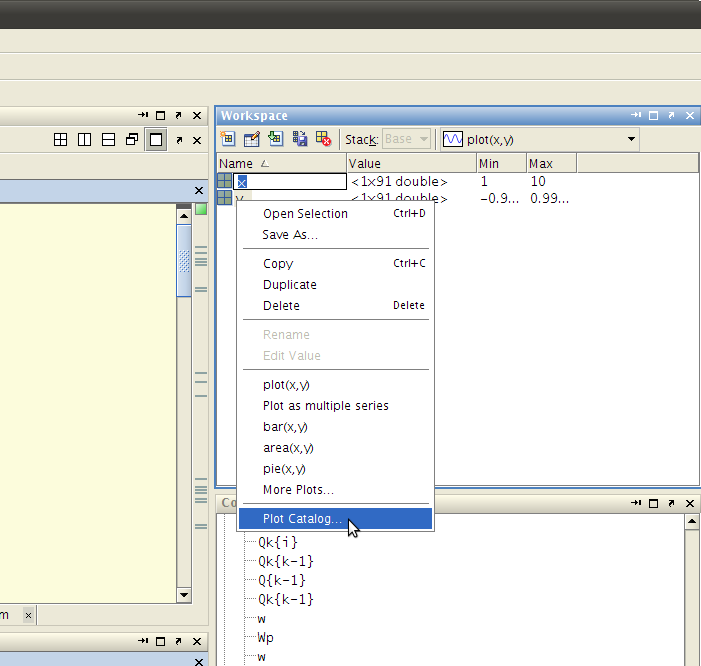
\includegraphics[width=0.6\linewidth]{./Screenshot-MATLAB_Worspace_plot.png}
  \end{figure}
}
\frame[containsverbatim]
{
  \frametitle{Типы графиков}
\begin{figure}[h]
 \centering
 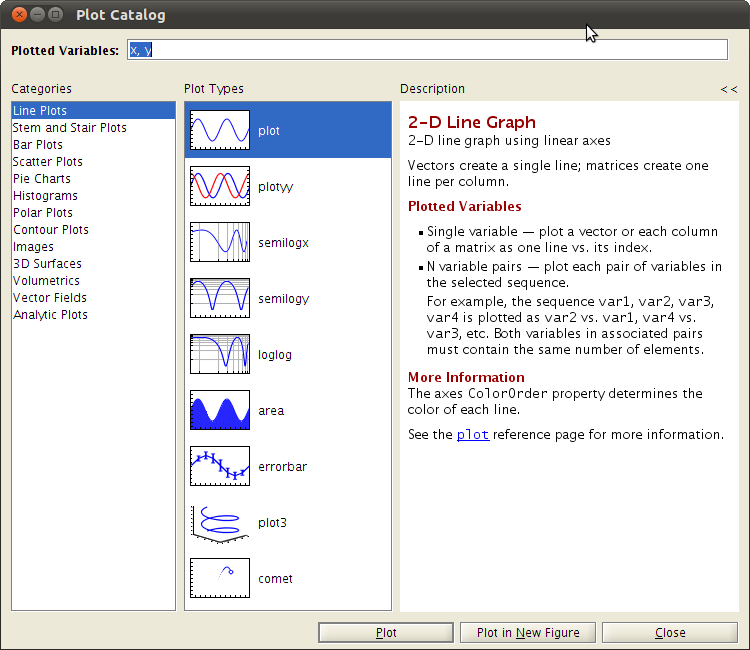
\includegraphics[width=0.6\linewidth]{./Screenshot-Plot_Catalog.png}
 % Screenshot-Plot Catalog.png: 750x650 pixel, 72dpi, 26.46x22.93 cm, bb=0 0 750 650
\end{figure}
}


\frame[containsverbatim]
{
\frametitle{График функции-выражения}
\begin{columns}
\column{0.5\linewidth}  
Для построения графиков функций, заданных выражением (m-файл, анонимная функция), используется функция \matcode{fplot}: 
\begin{lstlisting}
function y = myfun(x)
    y = sin(x).^2 + x;
end
\end{lstlisting}
\begin{lstlisting}
fplot(@myfun, [0 2*pi])
\end{lstlisting}
\column{0.5\linewidth}

\includegraphics[width=1\textwidth]{fplot.png}
\end{columns}
}


\frame[containsverbatim]
{
\frametitle{Функция plot}
\begin{columns}
\column{0.5\linewidth}
Для построения графиков табличных функций используется функция \matcode{plot}.
\begin{lstlisting}
x=0:0.1:5;
y=sin(x);
plot(x,y);
\end{lstlisting}
\column{0.5\linewidth}
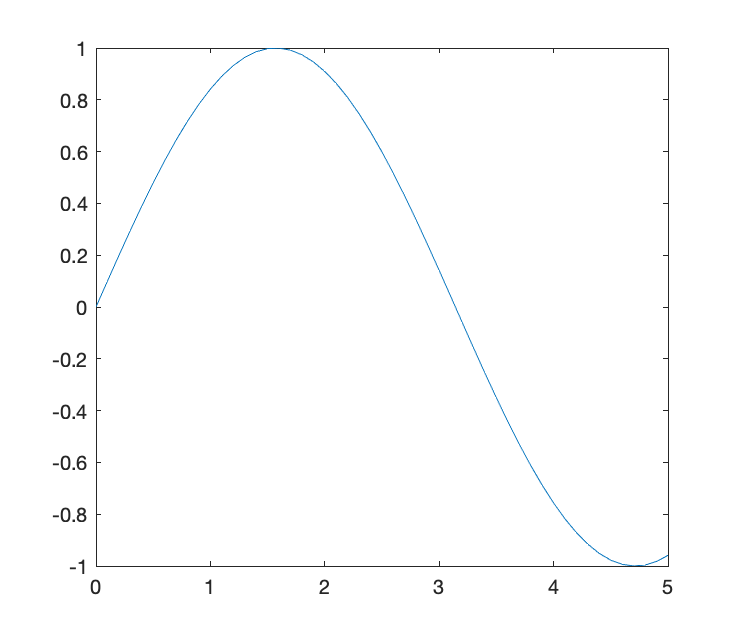
\includegraphics[width=1\textwidth]{plot.png}
\end{columns}
}


\frame[containsverbatim]
{
\frametitle{Функция plot}
\begin{columns}
\column{0.5\linewidth}
Несколько графиков на одном рисунке 
\begin{lstlisting}
x=0:0.1:5;
y1=sin(x);
y2=sin(x);
plot(x,y1,x,y2);
\end{lstlisting}
\column{0.5\linewidth}
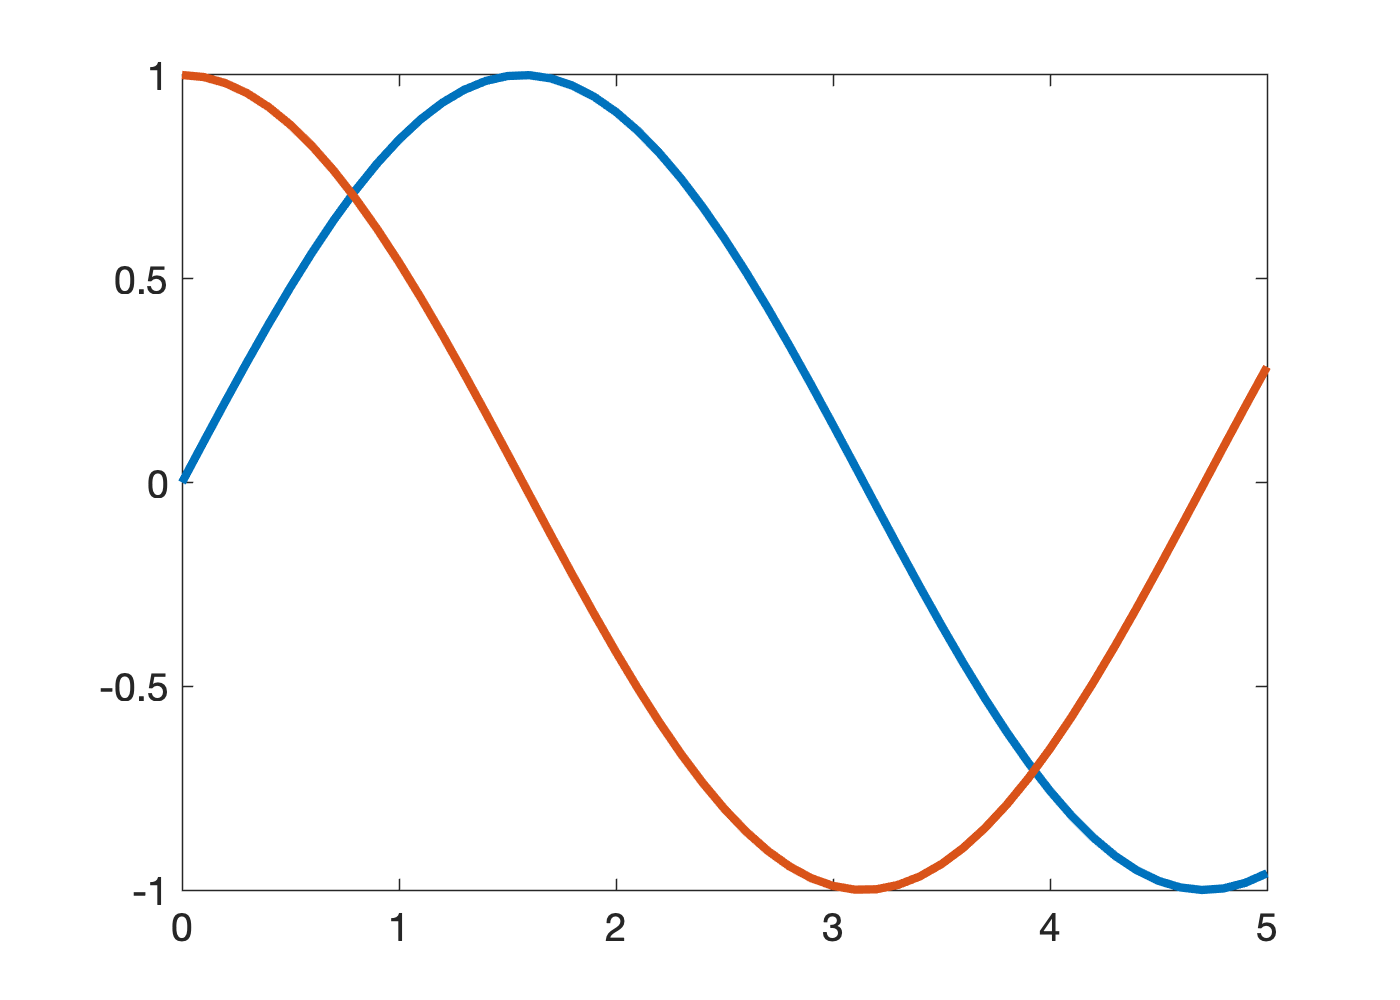
\includegraphics[width=1\textwidth]{plot2.png}
\end{columns}
}

\frame[containsverbatim]
{
\frametitle{Функция plot}
\begin{columns}
\column{0.5\linewidth}
Построение нескольких графиков на одном рисунке, используя директивы \emph{hold on}, \emph{hold off}:
\begin{lstlisting}
x=0:0.1:5;
y1=sin(x);
plot(x,y1);

hold on;

y2=sin(x);
plot(x,y2);

hold off;
\end{lstlisting}
\column{0.5\linewidth}
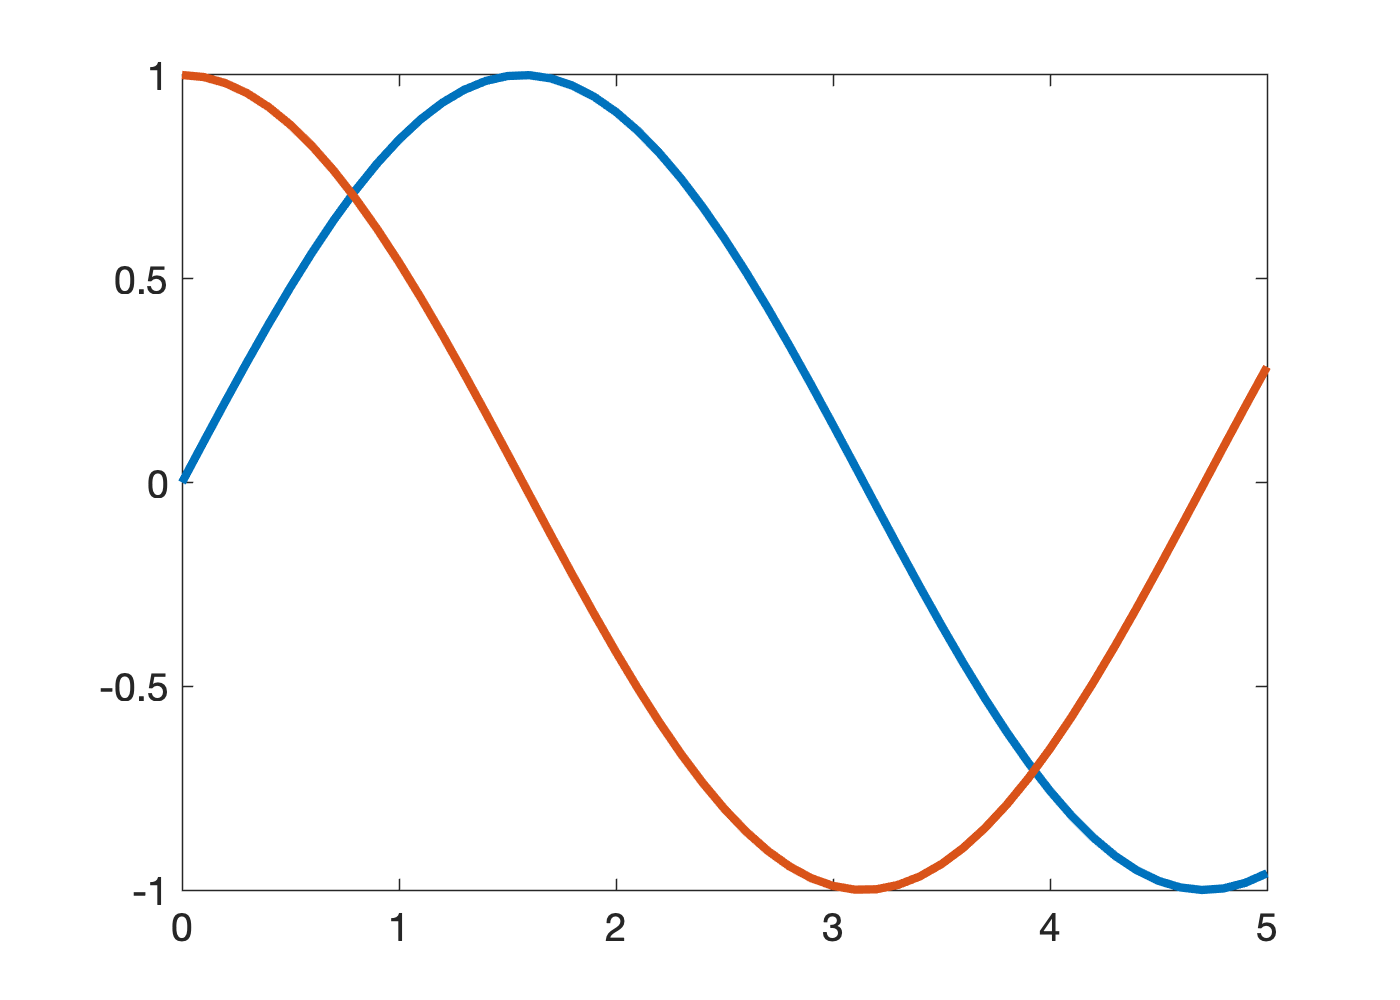
\includegraphics[width=1\textwidth]{plot2.png}
\end{columns}
}


\frame[containsverbatim]
{
\frametitle{Свойства линий}
\begin{columns}
\column{0.5\linewidth}
Третим аргументом функции \matcode{plot} можно передать строковую константу, описывающую свойства графика: цвет, тип маркера и тип линии.  
\begin{lstlisting}
x=0:0.1:5;
y=sin(x);
plot(x,y,'ro-.');
\end{lstlisting}
Тип линии
\begin{verbatim}
-   сплошная 
--  штрих 
-.  штрих-точка
:   точки
\end{verbatim}
\column{0.5\linewidth}
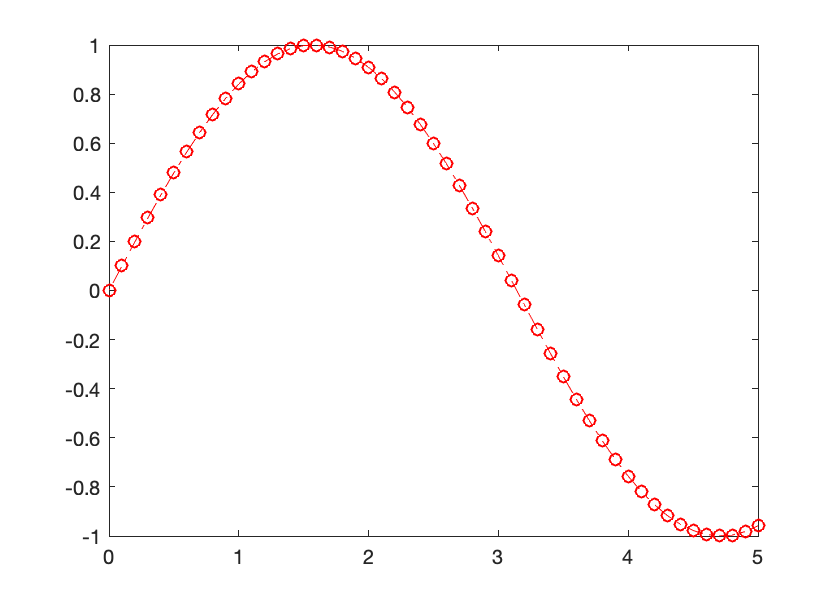
\includegraphics[width=1\textwidth]{plot_style.png}
\end{columns}
}

\begin{frame}[c]
\frametitle{Коды цвета}
\centering
\begin{tabular}{c|l}
Символ цвета & Цвет графика \\
\hline
y & желтый (\emph{y}ellow) \\
g & зеленый (\emph{g}reen) \\
m & малиновый (\emph{m}agenta) \\
b & синий (\emph{b}lue) \\
c & циановый (\emph{c}yan) \\
w & белый (\emph{w}hite) \\
r & красный (\emph{r}ed) \\
k & черный (blac\emph{k}) 
\end{tabular}
\end{frame}

\begin{frame}[c]
\frametitle{Маркеры}
\centering
\begin{tabular}{c|l}
Символ & Маркер \\
\hline
. & точка \\
o & кружок \\
x & косоугольный крест \\
+ & прямоугольный крест \\
* & снежинка \\
s & квадрат \\
d & ромб \\
v & треугольник вершиной вниз \\
$\wedge$ & треугольник вершиной вверх\\
> & треугольник вершиной вправо \\
< & треугольник вершиной влево \\
p & пятиугольник \\
h & шестиугольник 
\end{tabular}
\end{frame}

\begin{frame}[fragile]\frametitle{Стили}
\begin{lstlisting}
x = 1:0.5:10; 
subplot(311);plot(x,sin(x),'r-');
subplot(312);plot(x,sin(x),'g-.');
subplot(313);plot(x,sin(x),'ko--');
\end{lstlisting}
\begin{center}
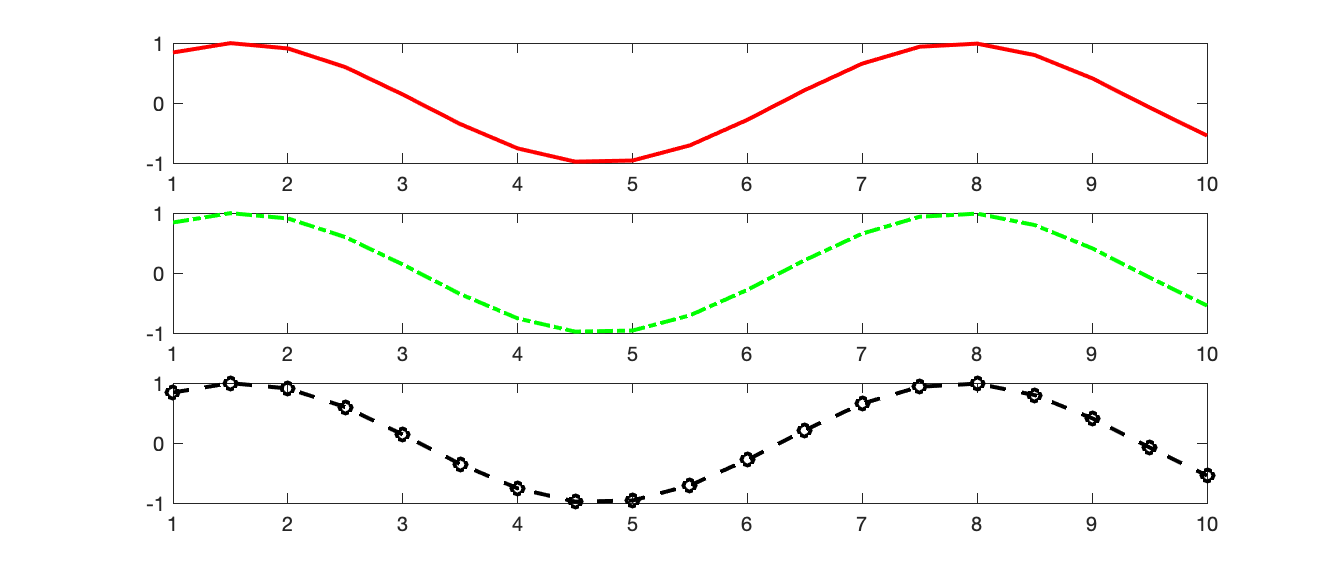
\includegraphics[width=0.9\textwidth]{plot_style_2.png}
\end{center}
\end{frame}

\frame[containsverbatim]
{
  \frametitle{Подписи к осям}
\begin{lstlisting}
plot(x,y1,x,y2);
grid on;
title('Скорости точек 1 и 2');
xlabel('t, c');
xlabel('v, м/c');
legend('точка 1','точка 2',pos);
\end{lstlisting}
Последний необязательный аргумент функции \matcode{legend} может задавать положении ``легенды'' в окне графика: 
\begin{itemize}
  \item -1 - вне графика
  \item 0 - лучшее расположение
  \item \textbf{1},2,3,4 - от верхнего правого до нижнего правого угла (по часовой стрелке)
\end{itemize}
}

\begin{frame}[fragile]
\frametitle{Границы осей}
При построении графика функции MATLAB  автоматически выбирает масштаб осей. Для ``ручного'' управления используются функции
\begin{itemize}
  \item \matcode{xlim([xmin, xmax])} 
  \item \matcode{ylim([ymin, ymax])}
\end{itemize}
\end{frame}

% \section{Комбинирование графиков}

\frame[containsverbatim]
{
\frametitle{Комбинирование графиков}
Создание нового окна для графика - команда \matcode{figure}:
\begin{lstlisting}
figure;
plot(t,x1);
figure;
plot(t,x2);
\end{lstlisting}
Последнее созданное окно становится текущим, команды форматирования графика (\matcode{title(..),colormap(...)}) влияют на график в этом окне. 
}

\frame[containsverbatim]
{
\frametitle{Функция subplot}
Функция \matcode{subplot(mnp)} или \matcode{subplot(m, n, p)}, где mnp - 3 цифры, производит разбивку графического окна (\matcode{figure}) на несколько областей, создавая при этом новые объекты axes.
\begin{itemize}
  \item m указывает, на сколько частей разбивается окно по горизонтали,
  \item n - по вертикали,
  \item p - номер подокна, куда будет выводиться после функции,
\end{itemize} 
}

\begin{frame}[fragile]
\frametitle{subplot}
\begin{lstlisting}
x  = linspace(0,2*pi,100);
y1 = sin(x);
y2 = cos(x);
y3 = tan(x);
y4 = cot(x);

subplot(2,2,1);
plot(x,y1); title('sin');ylim([-1,1]);
subplot(2,2,2);
plot(x,y2); title('cos');ylim([-1,1]);
subplot(2,2,3);
plot(x,y3); title('tan');ylim([-5,5]);
subplot(2,2,4);
plot(x,y4); title('ctg');ylim([-5,5]);
\end{lstlisting}
\end{frame}

\begin{frame}[t]
\frametitle{subplot}
\centering
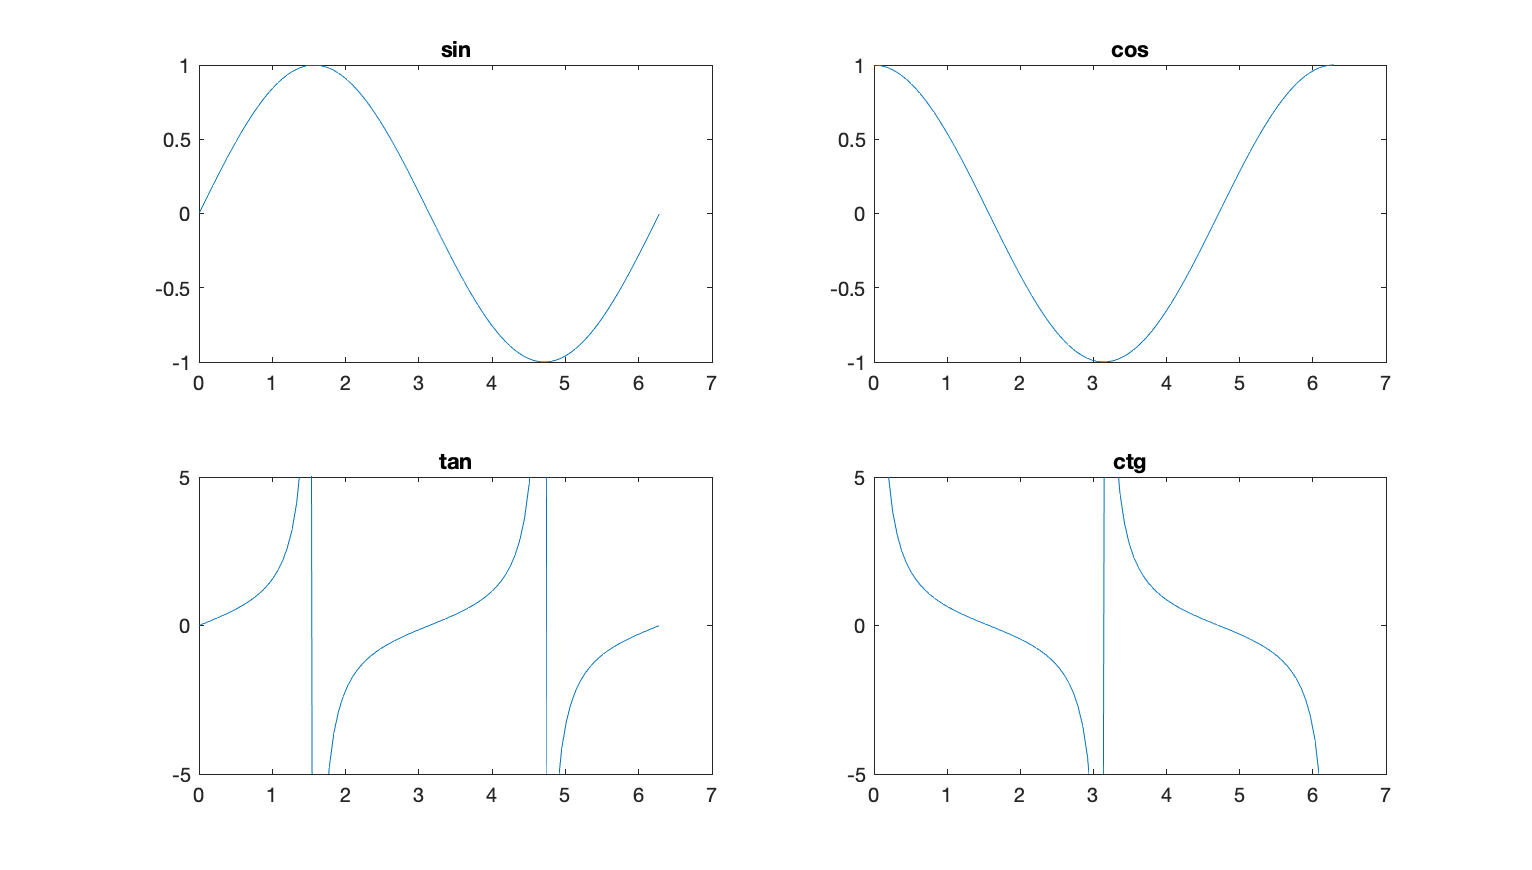
\includegraphics[width=1.0\textwidth]{subplot.png}
\end{frame}









%
% Графики в логарифмических масштабах
%
\frame[containsverbatim]
{ 
\frametitle{Логарифмическая шкала} 
\begin{itemize}
   \item \matcode{loglog} - логарифмический масштаб по обеим осям. 
   \item \matcode{semilogx} - логарифмический масштаб по оси абсцисс.
   \item \matcode{semilogy} - логарифмический масштаб по оси ординат.   
  \end{itemize}
\begin{lstlisting}
x=0.1:0.01:10;    
y=log(0.5*x);
g=sin(log(x));
semilogx(x,y,'r-', x,g, 'g:');
\end{lstlisting}
}

\begin{frame}[c]\frametitle{Логарифмическая шкала}
\begin{figure}[htbp]
      \centering
      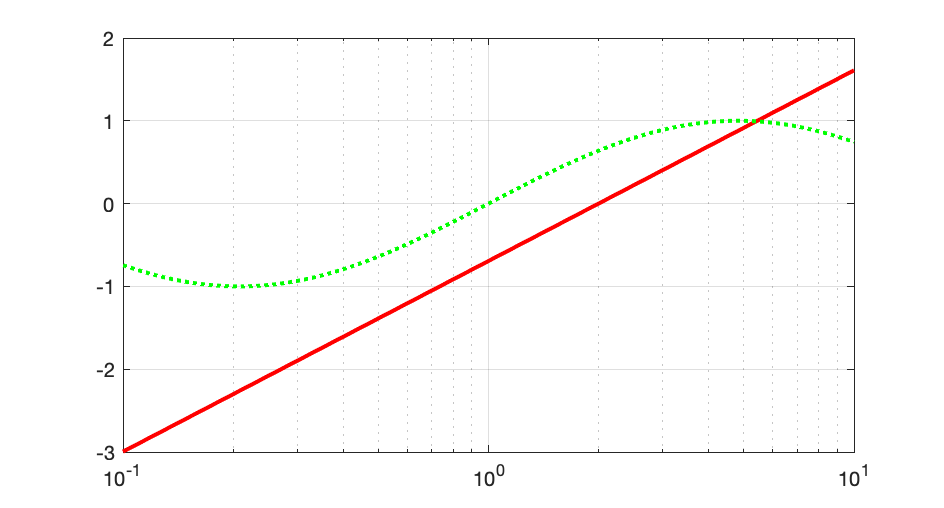
\includegraphics[width=1\textwidth]{log.png}
\end{figure}    
\end{frame}

\begin{frame}[t]
\frametitle{Иерархия графических классов}
      \centering
      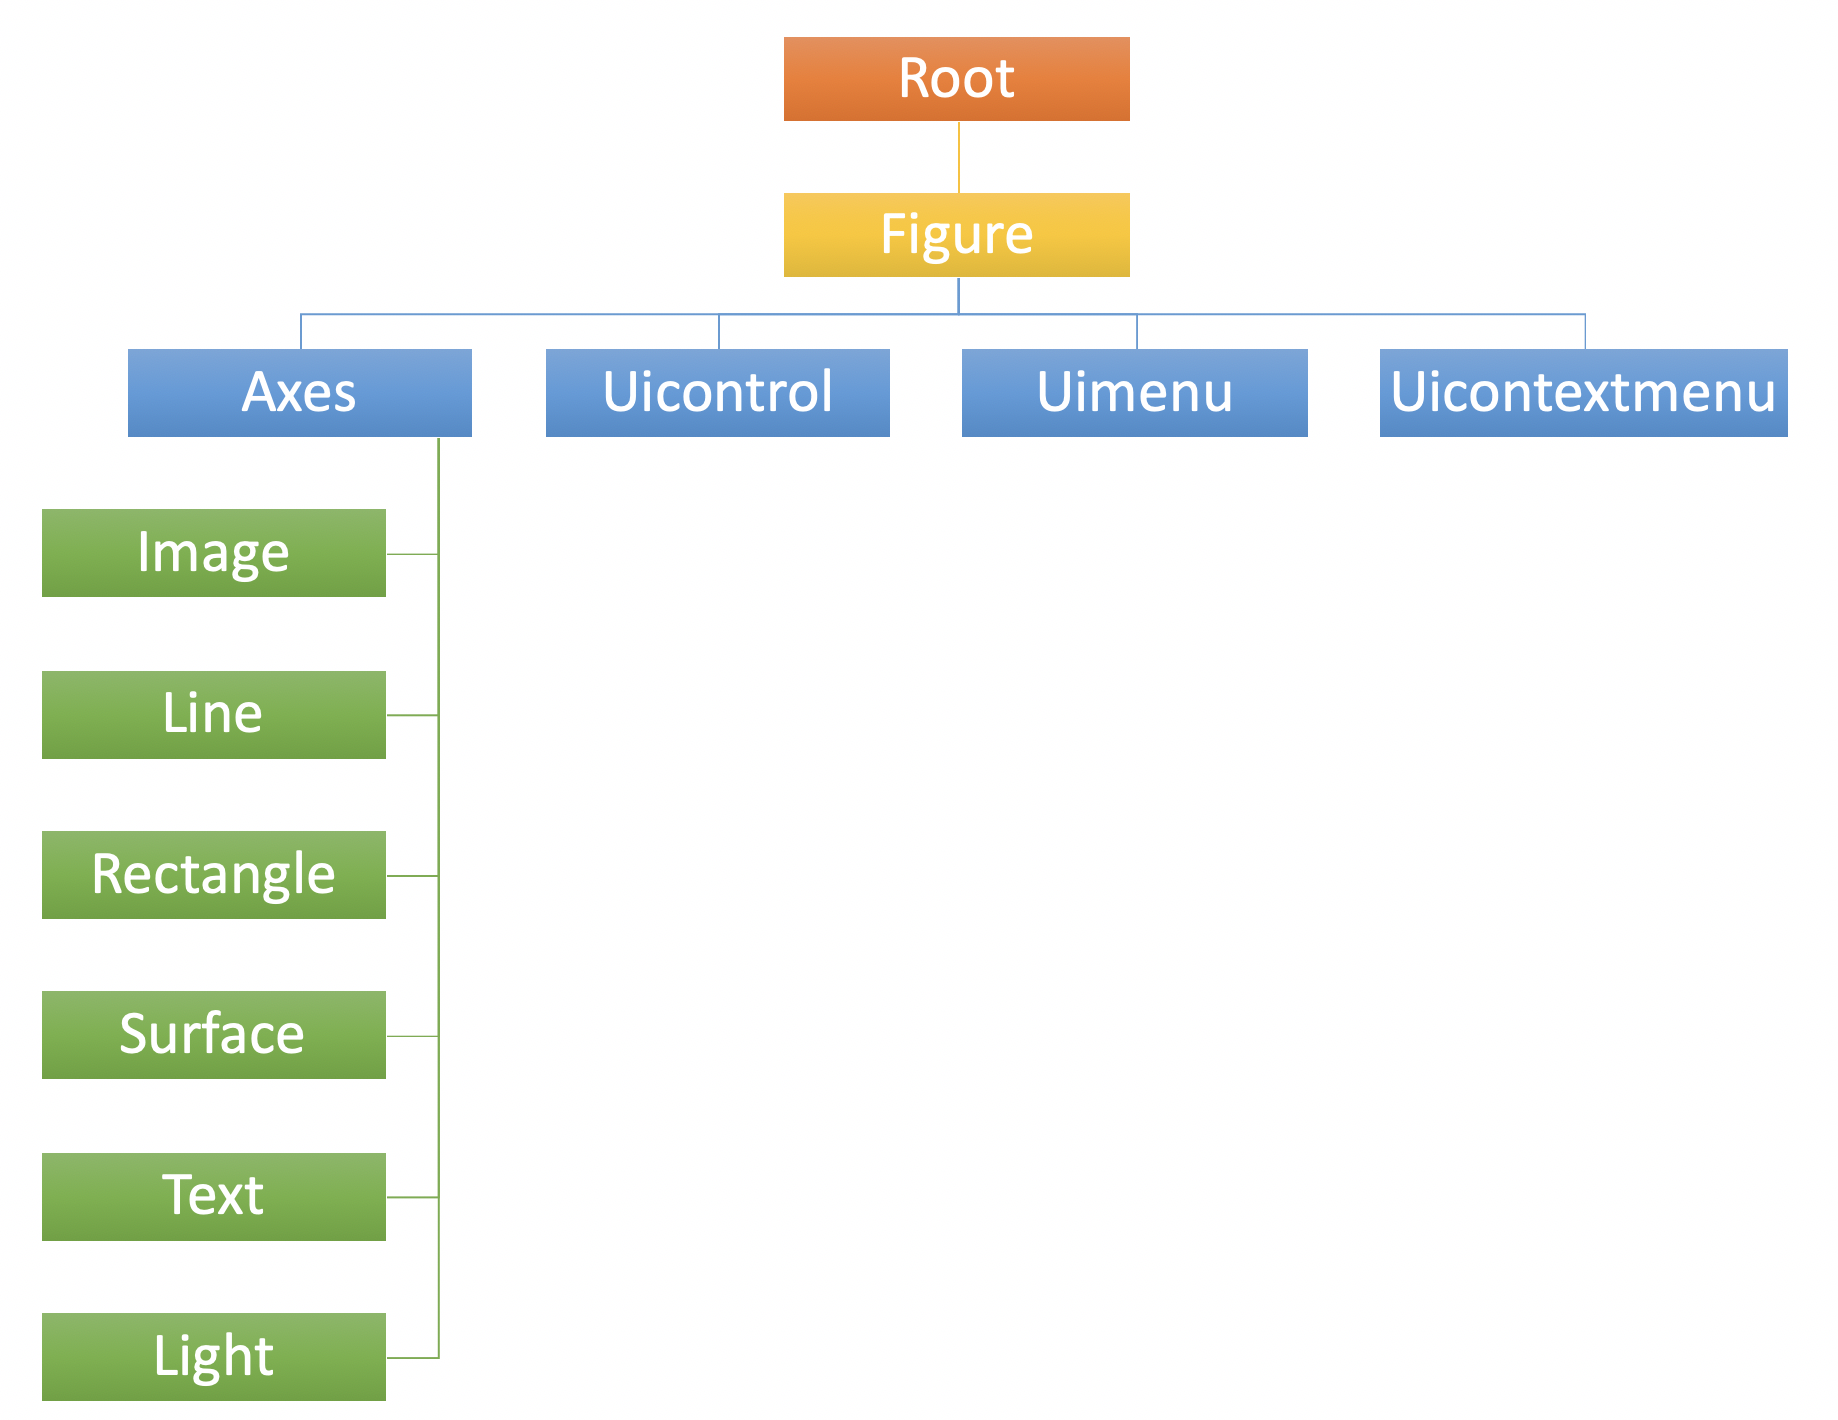
\includegraphics[width=0.8\textwidth]{tree.png}
\end{frame}

\begin{frame}[c]
\frametitle{Иерархия графических классов}
\begin{itemize}
  \item Root \\
  Экран компьютера
  \item Figure \\
  Окно с рисунком. 
  \item Axes \\
  Координатная область, в которой отображаются графики, текст, ... (результаты работы функций \emph{plot}, \emph{line}, принадлежат объекту \emph{axes}.)
\end{itemize}
\end{frame}


\begin{frame}[c,containsverbatim]
\frametitle{figure и axes}
\begin{columns}
\column{0.5\linewidth}
\begin{lstlisting}
figure('Color','white');
x = 0:0.1:5;
plot(x,sin(x))
\end{lstlisting}      
\begin{lstlisting}
x = 0:0.1:5;
plot(x,sin(x));
\end{lstlisting}      
Изменяем свойства текущего объекта figure (gcf - ссылка на текущий активный объект figure):
\begin{lstlisting}
set(gcf,'Color','white');
\end{lstlisting}      
Изменяем свойства текущего объекта axes (gca - ссылка на текущий активный объект axes): 
\begin{lstlisting}
set(gca,'FontSize',16);
\end{lstlisting}      
\column{0.5\linewidth}
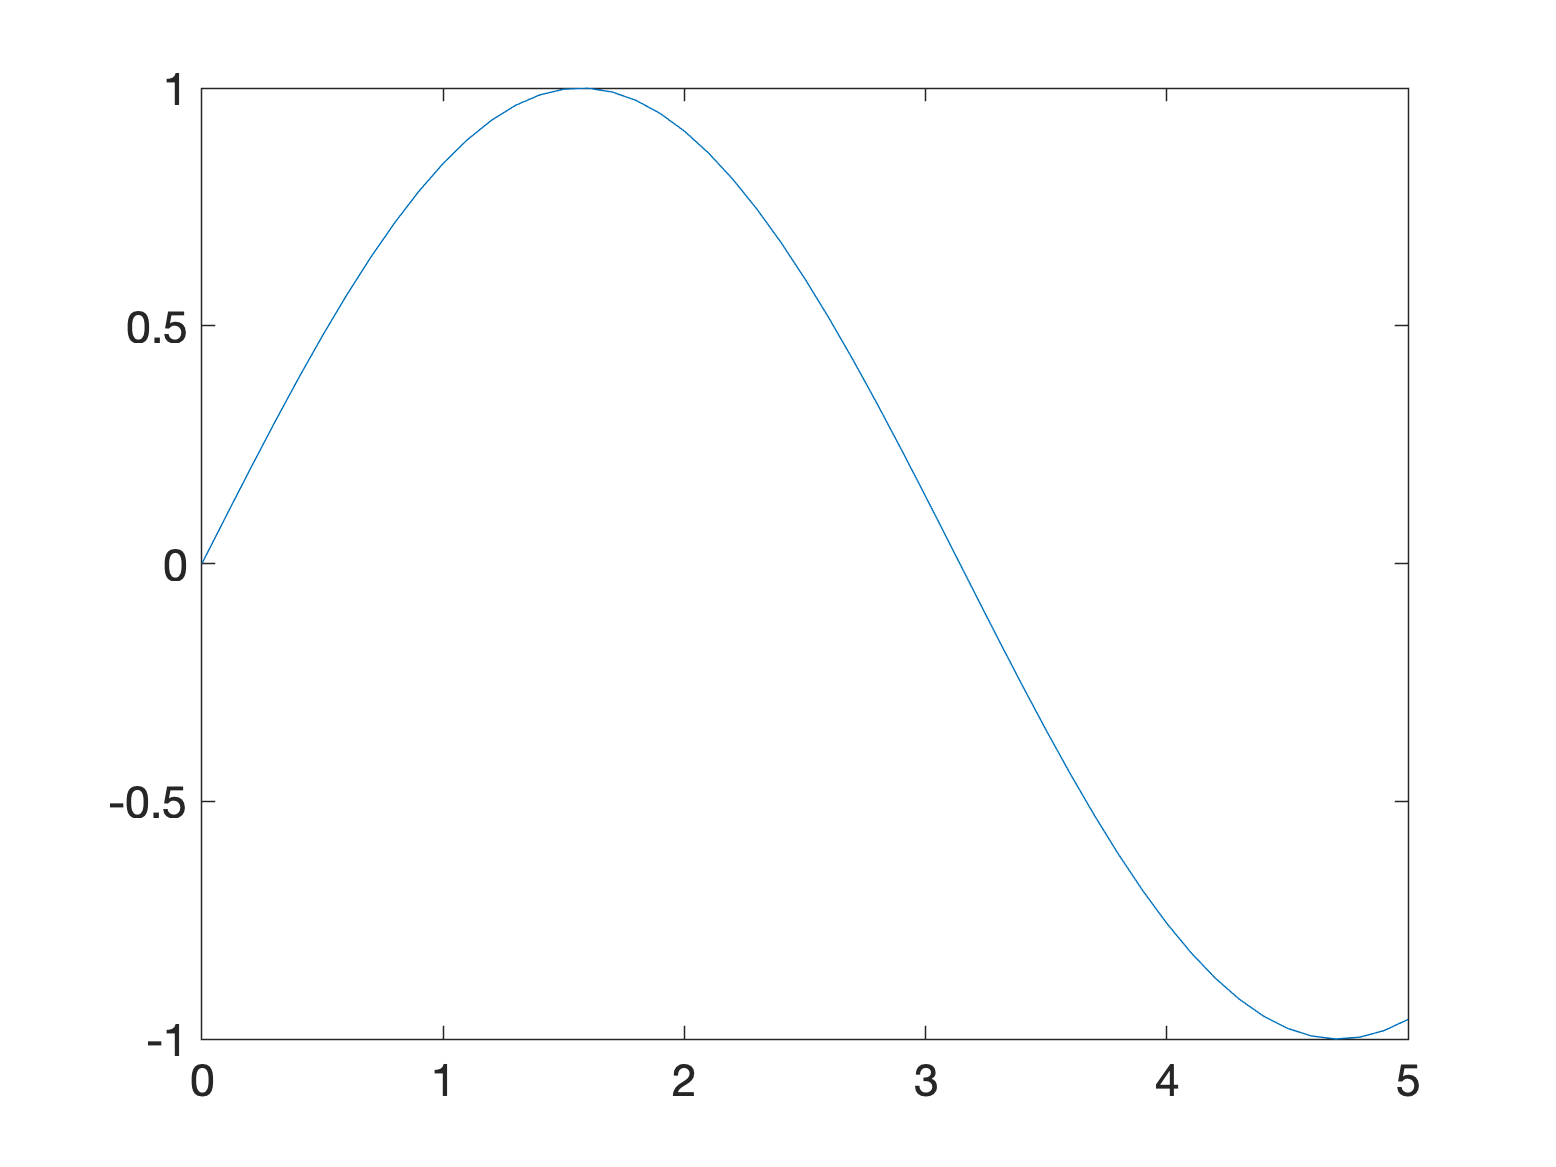
\includegraphics[width=1\textwidth]{plot_figure.png}
\end{columns}
\end{frame}


\begin{frame}[c,containsverbatim]
\frametitle{figure и axes}
\begin{columns}
\column{0.5\linewidth}
\begin{lstlisting}
figure('Color','white');
x = 0:0.1:5;
h = plot(x,sin(x));
set(h,'LineWidth',2)
\end{lstlisting}      
\begin{lstlisting}
x = 0:0.1:5;
plot(x,sin(x),'LineWidth',2);
set(gcf,'Color','white');
set(gca,'FontSize',16);
\end{lstlisting}      
\column{0.5\linewidth}
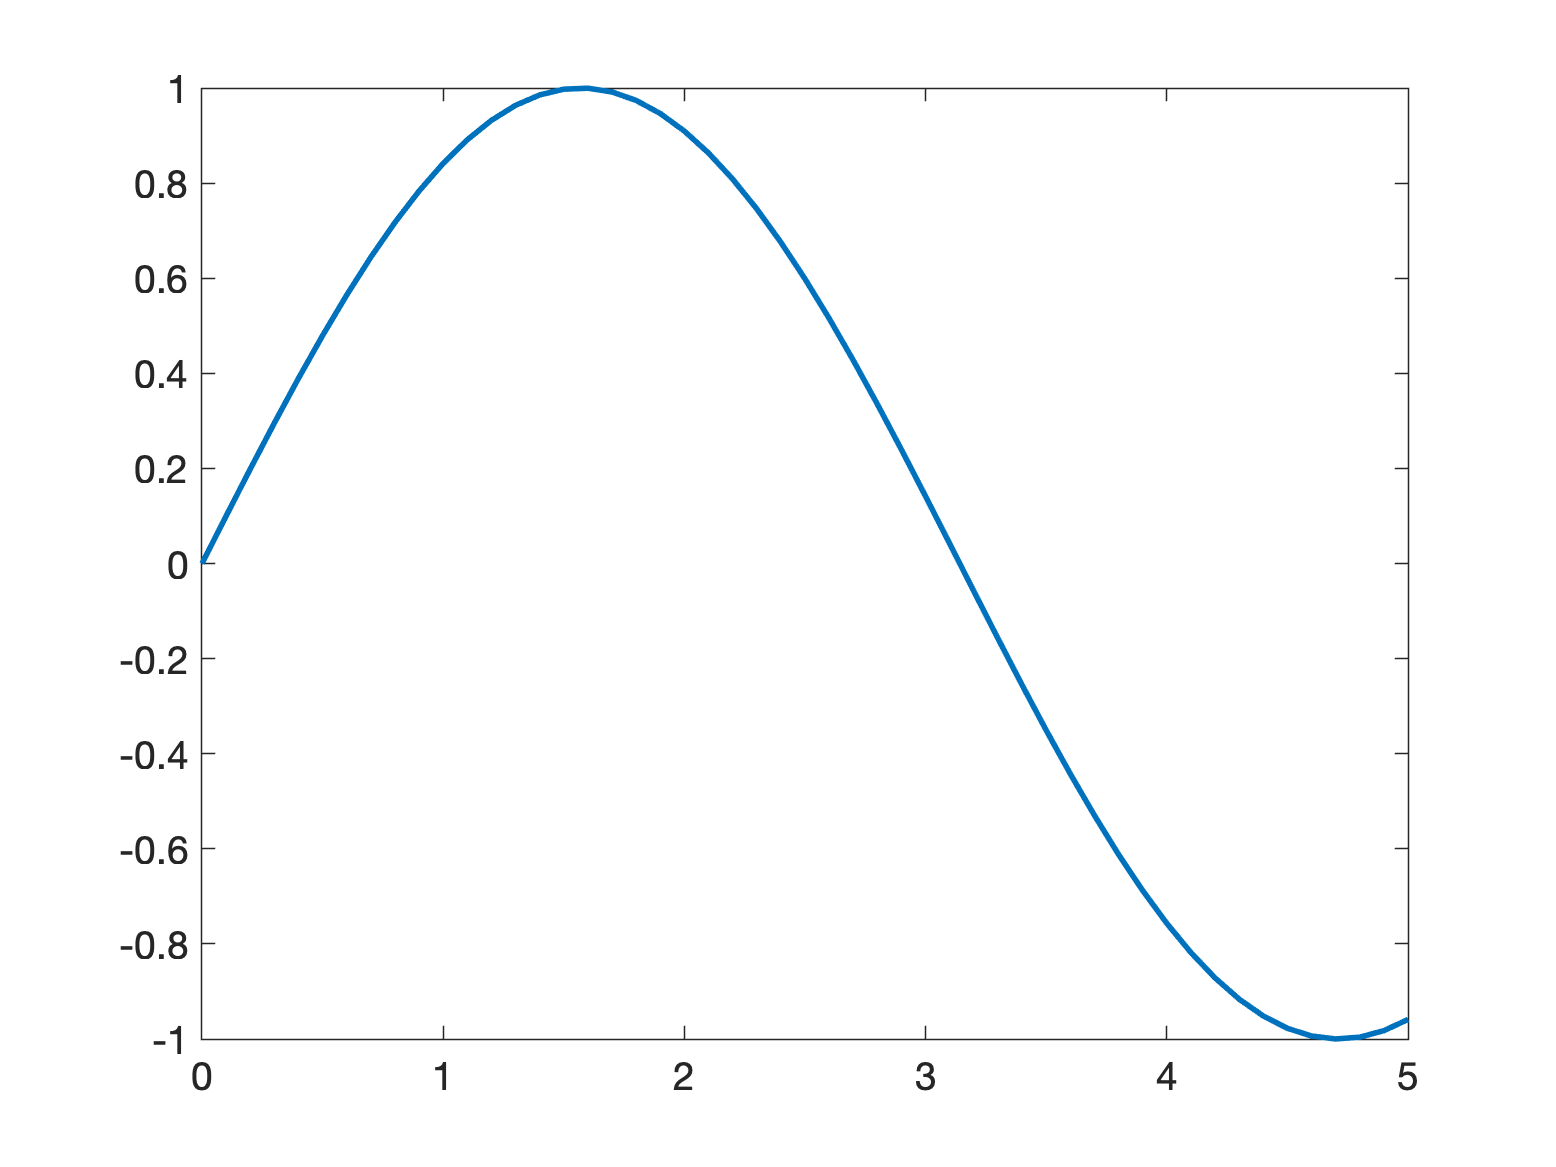
\includegraphics[width=1\textwidth]{plot_width.png}
\end{columns}
\end{frame}


\begin{frame}[c,containsverbatim]
\frametitle{\frametitle{Свойства объекта Line, принадлежащего axes}}
\begin{lstlisting}
x = 0:0.1:5;
h = plot(x,sin(x),'LineWidth',2);

>> h

  Line with properties:

              Color: [0 0.4470 0.7410]
          LineStyle: '-'
          LineWidth: 2
             Marker: 'none'
         MarkerSize: 6
    MarkerFaceColor: 'none'
              XData: [1×51 double]
              YData: [1×51 double]
              ZData: [1×0 double]
\end{lstlisting}
\end{frame}

\begin{frame}[c,containsverbatim]
\frametitle{figure и axes}
\begin{columns}
\column{0.5\linewidth}
\begin{lstlisting}
figure('Color','white');
x = 0:0.1:5;
h = plot(x,sin(x),x,cos(x));
set(gca,'FontSize',14)
set(h,{'LineWidth'},{2;4});
\end{lstlisting}      
\column{0.5\linewidth}
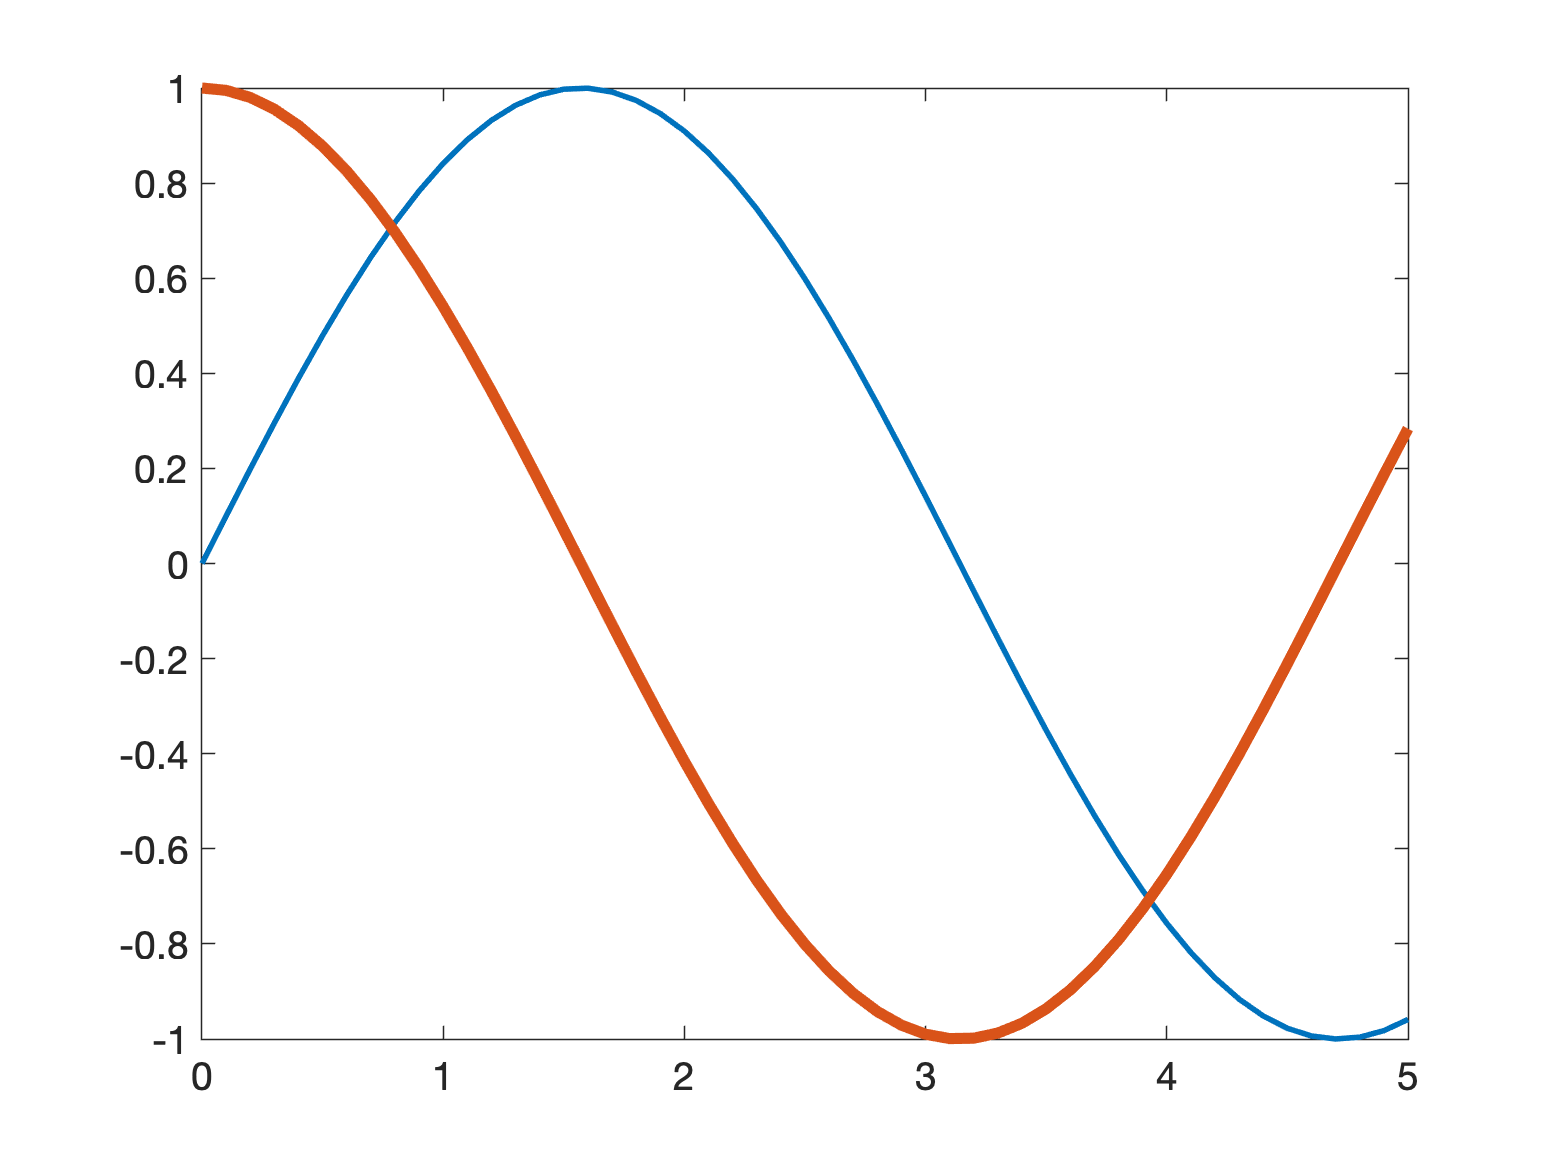
\includegraphics[width=1\textwidth]{plot_width_multiple.png}
\end{columns}
\end{frame}


\frame[containsverbatim]
{
\frametitle{Столбчатые диаграммы}
\begin{columns}
\column{.4\textwidth}  
\begin{lstlisting}
x=1:0.2:3;
y=sin(x);
bar(x,y);
\end{lstlisting}
\begin{lstlisting}
x=1:0.2:3;
y=sin(x);
bar(y);
\end{lstlisting}
\column{0.6\textwidth}  
\begin{center}
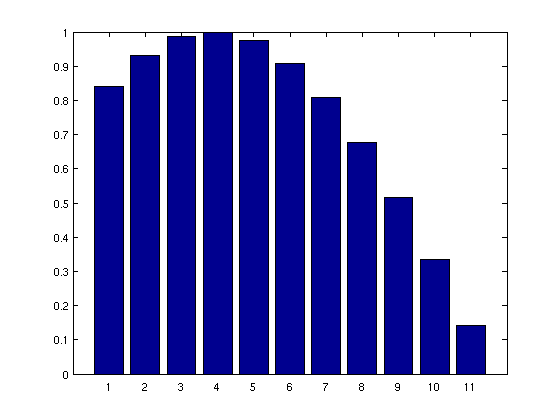
\includegraphics[width=1\linewidth]{./bar.png}
\end{center}
\end{columns}
}

\frame[containsverbatim]
{
\frametitle{Столбчатые диаграммы}
\begin{columns}
\column{.4\textwidth} 
Третий (второй) аргумент задает ширину столбца в долях от полной ширины 
\begin{lstlisting}
x=1:0.2:3;
y=sin(x);
bar(x,y,0.5);
\end{lstlisting}
\begin{lstlisting}
x=1:0.2:3;
y=sin(x);
bar(y,0.95);
\end{lstlisting}
\column{0.6\textwidth}  
\begin{center}
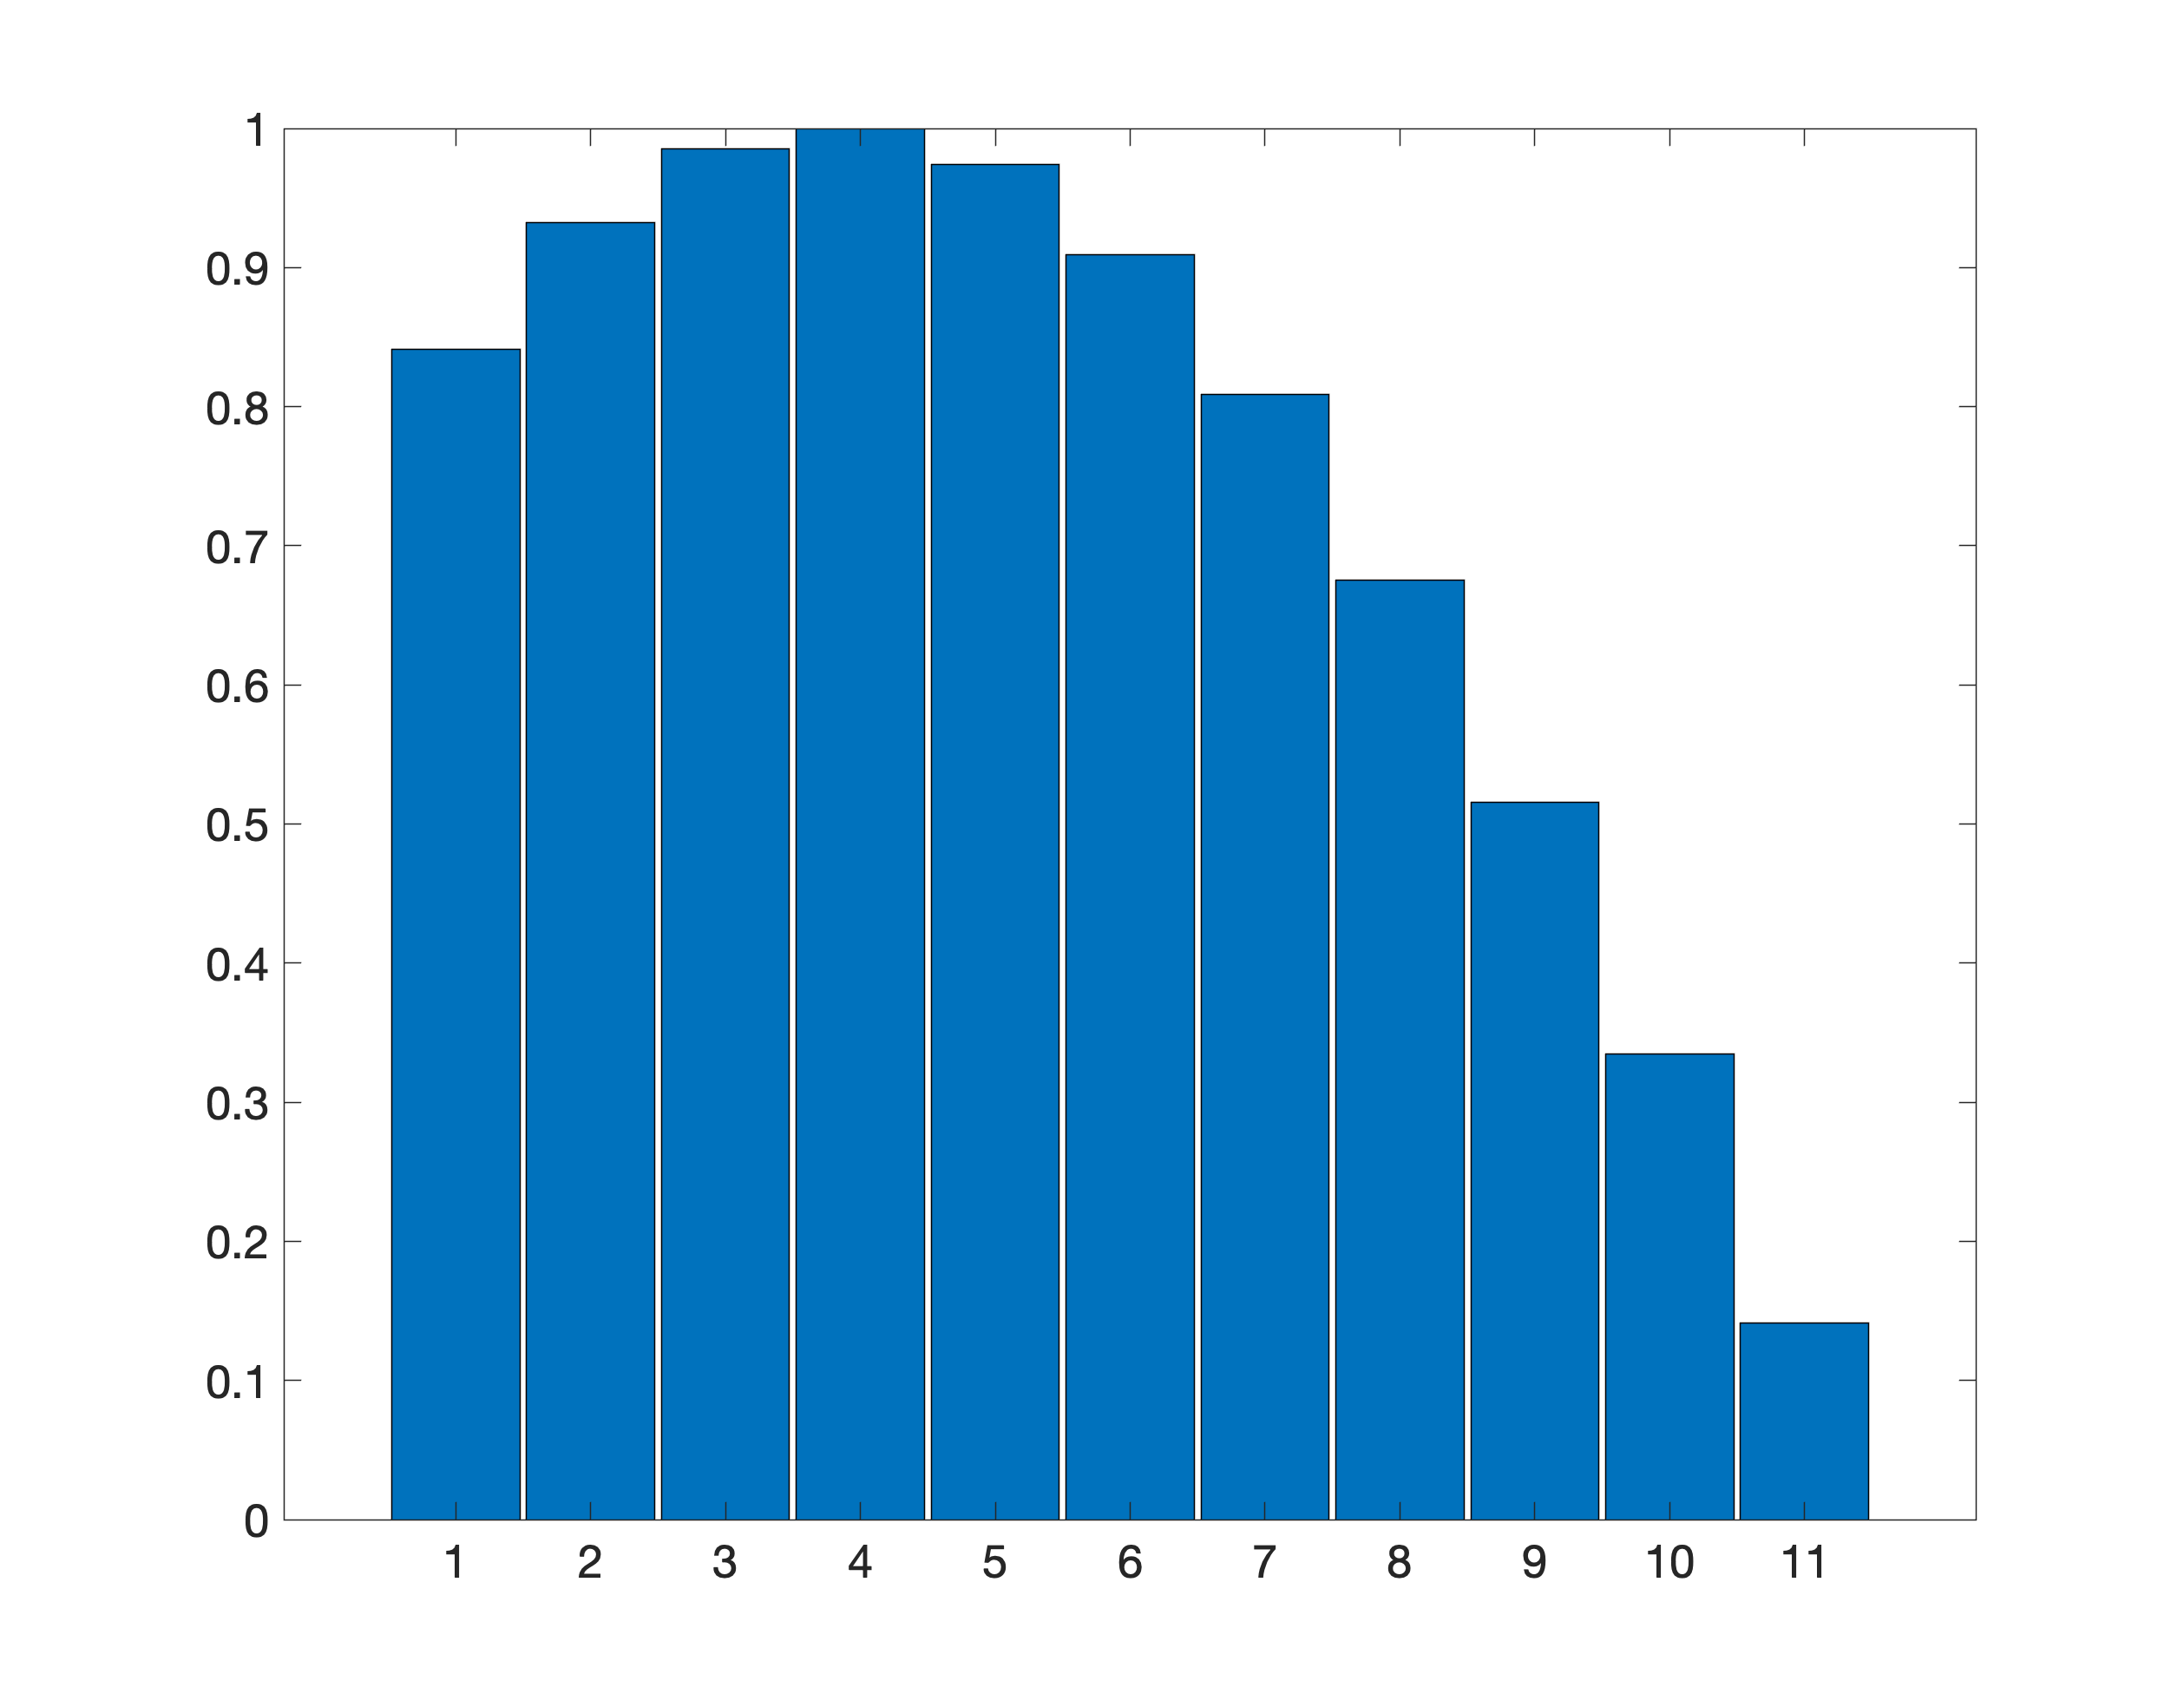
\includegraphics[width=1\linewidth]{./bar_width.png}
\end{center}
\end{columns}
}

\frame[containsverbatim]
{
\frametitle{Столбчатые диаграммы}
\begin{columns}
\column{.4\textwidth} 
Группы столбцов
\begin{lstlisting}
y = [2 2 3; 
     2 5 6; 
     2 8 9; 
     2 11 12];
bar(y);
\end{lstlisting}
\column{0.6\textwidth}  
\begin{center}
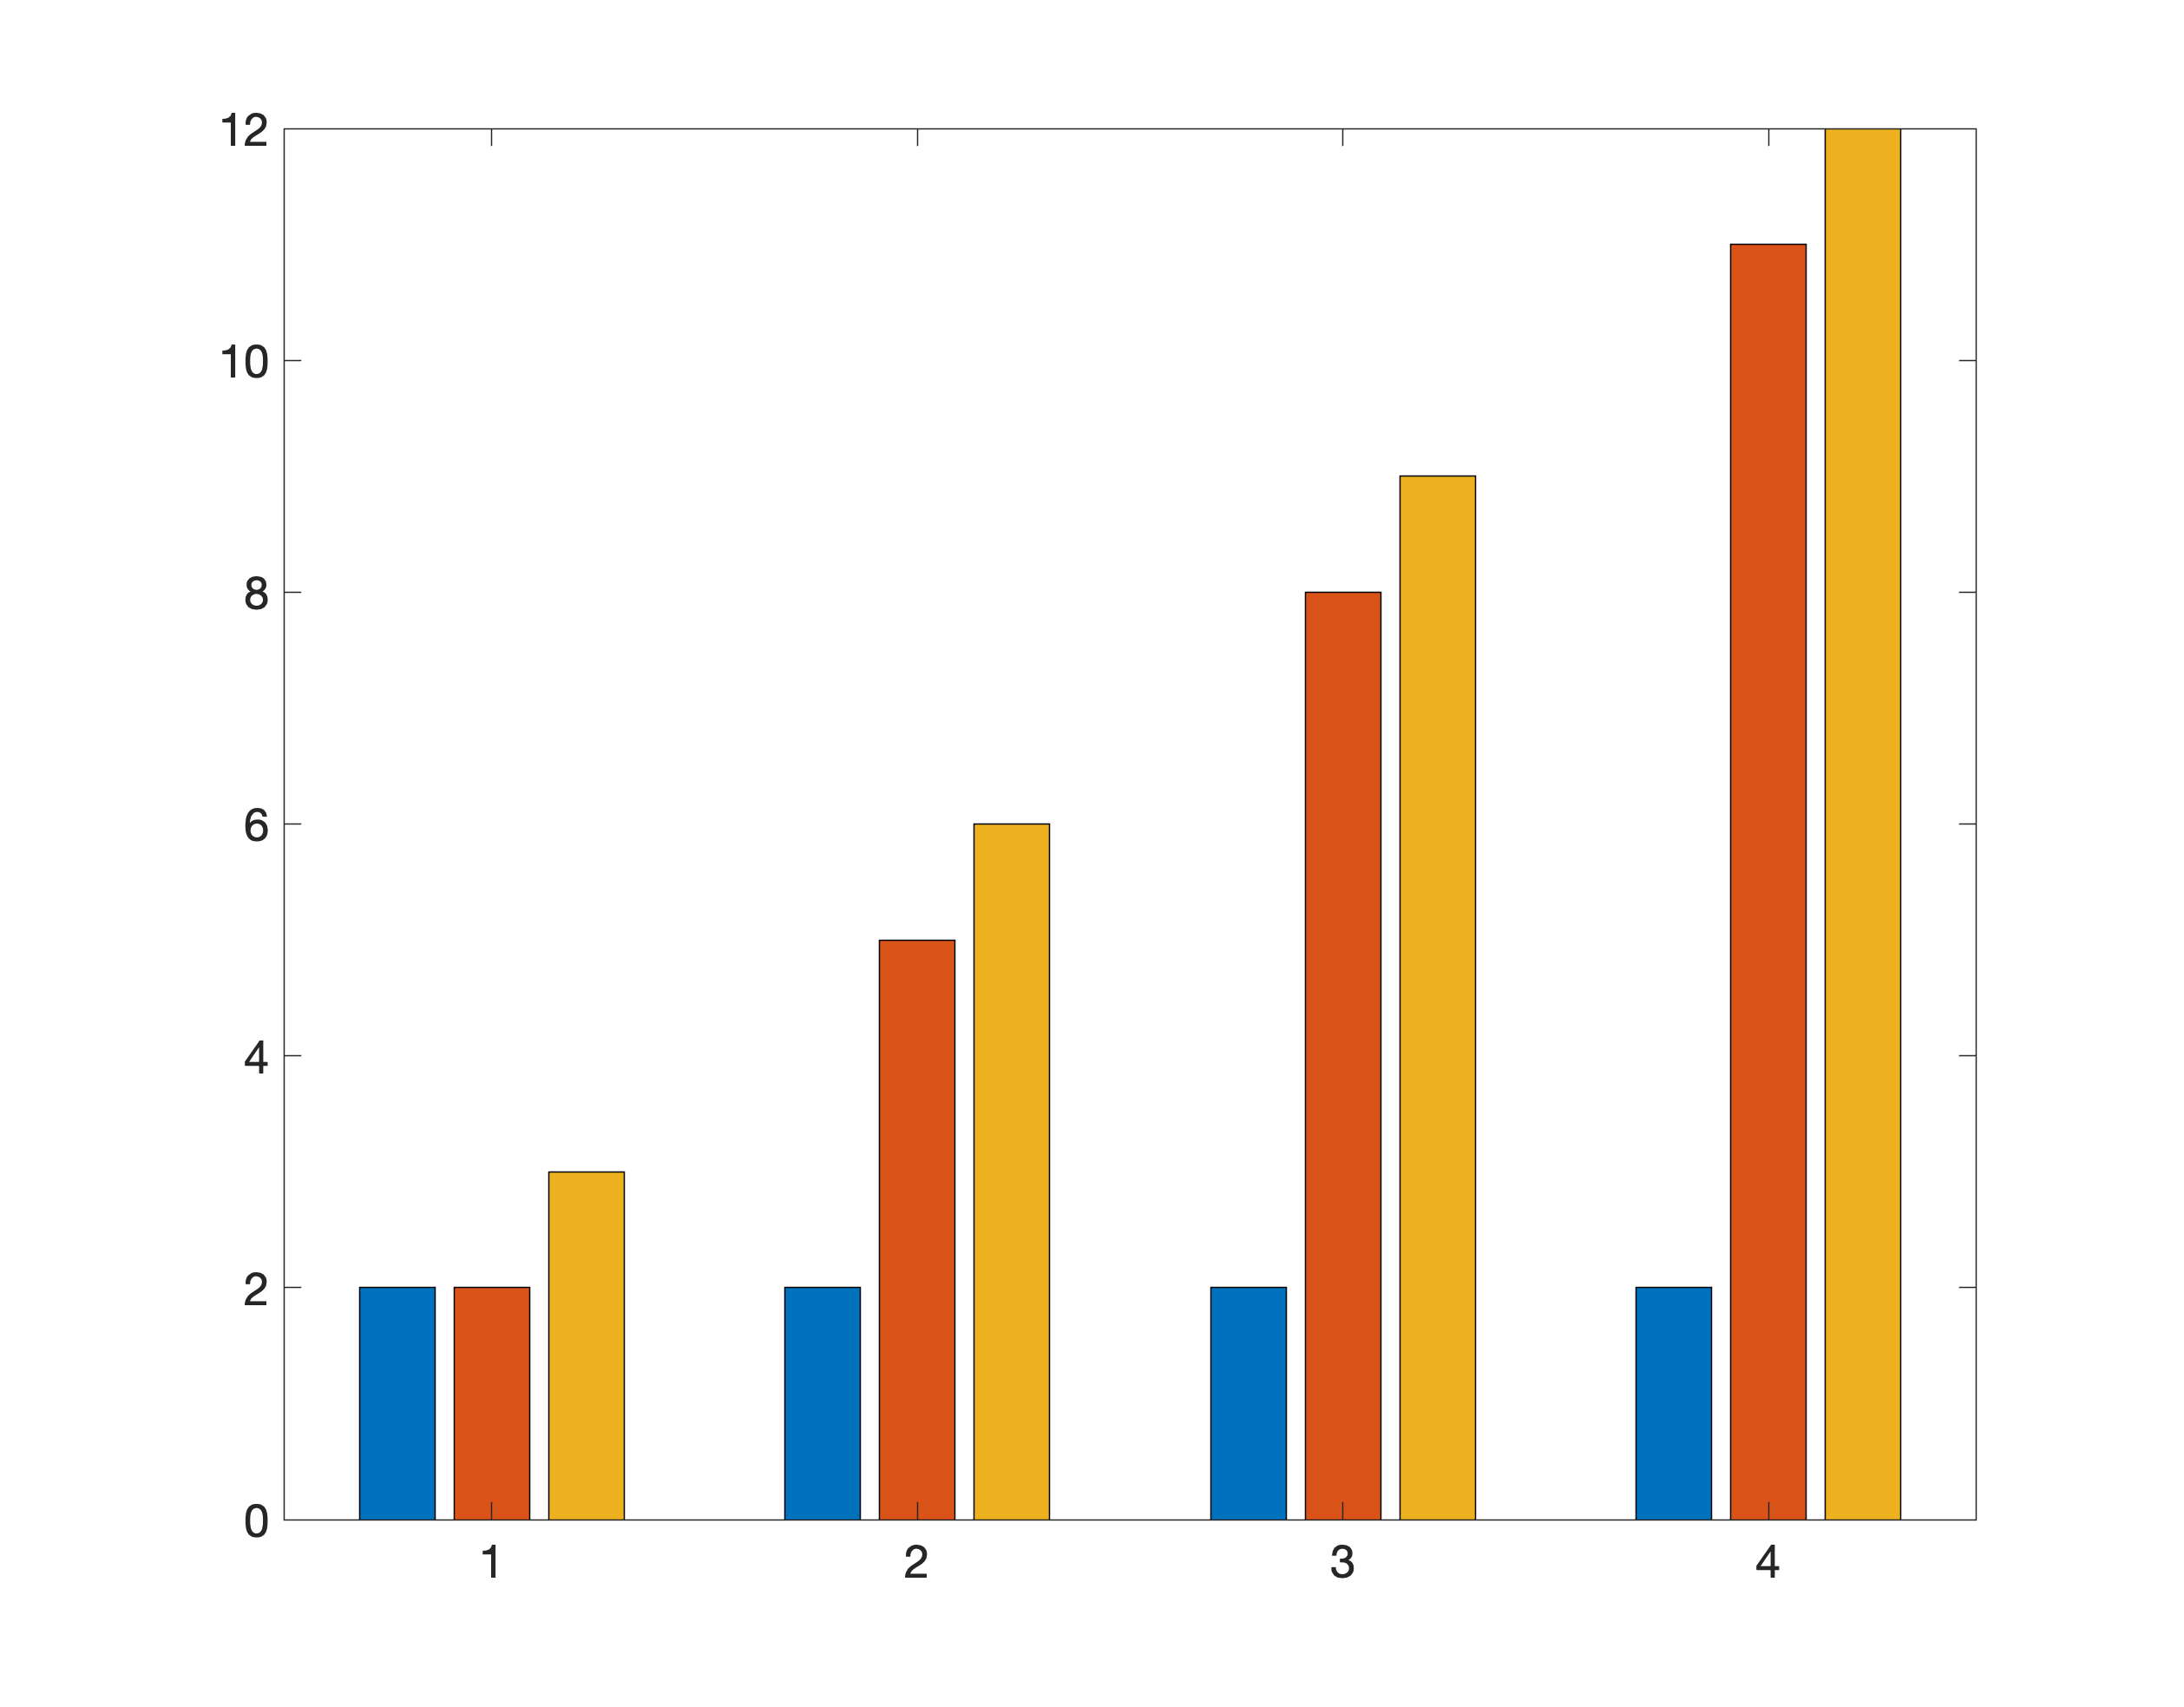
\includegraphics[width=1\linewidth]{./bar_group.png}
\end{center}
\end{columns}
}

\frame[containsverbatim]
{
\frametitle{Столбчатые диаграммы}
\begin{columns}
\column{.4\textwidth} 
Графики с накоплением
\begin{lstlisting}
y = [2 2 3; 
     2 5 6; 
     2 8 9; 
     2 11 12];
bar(y,'stacked')
\end{lstlisting}
\column{0.6\textwidth}  
\begin{center}
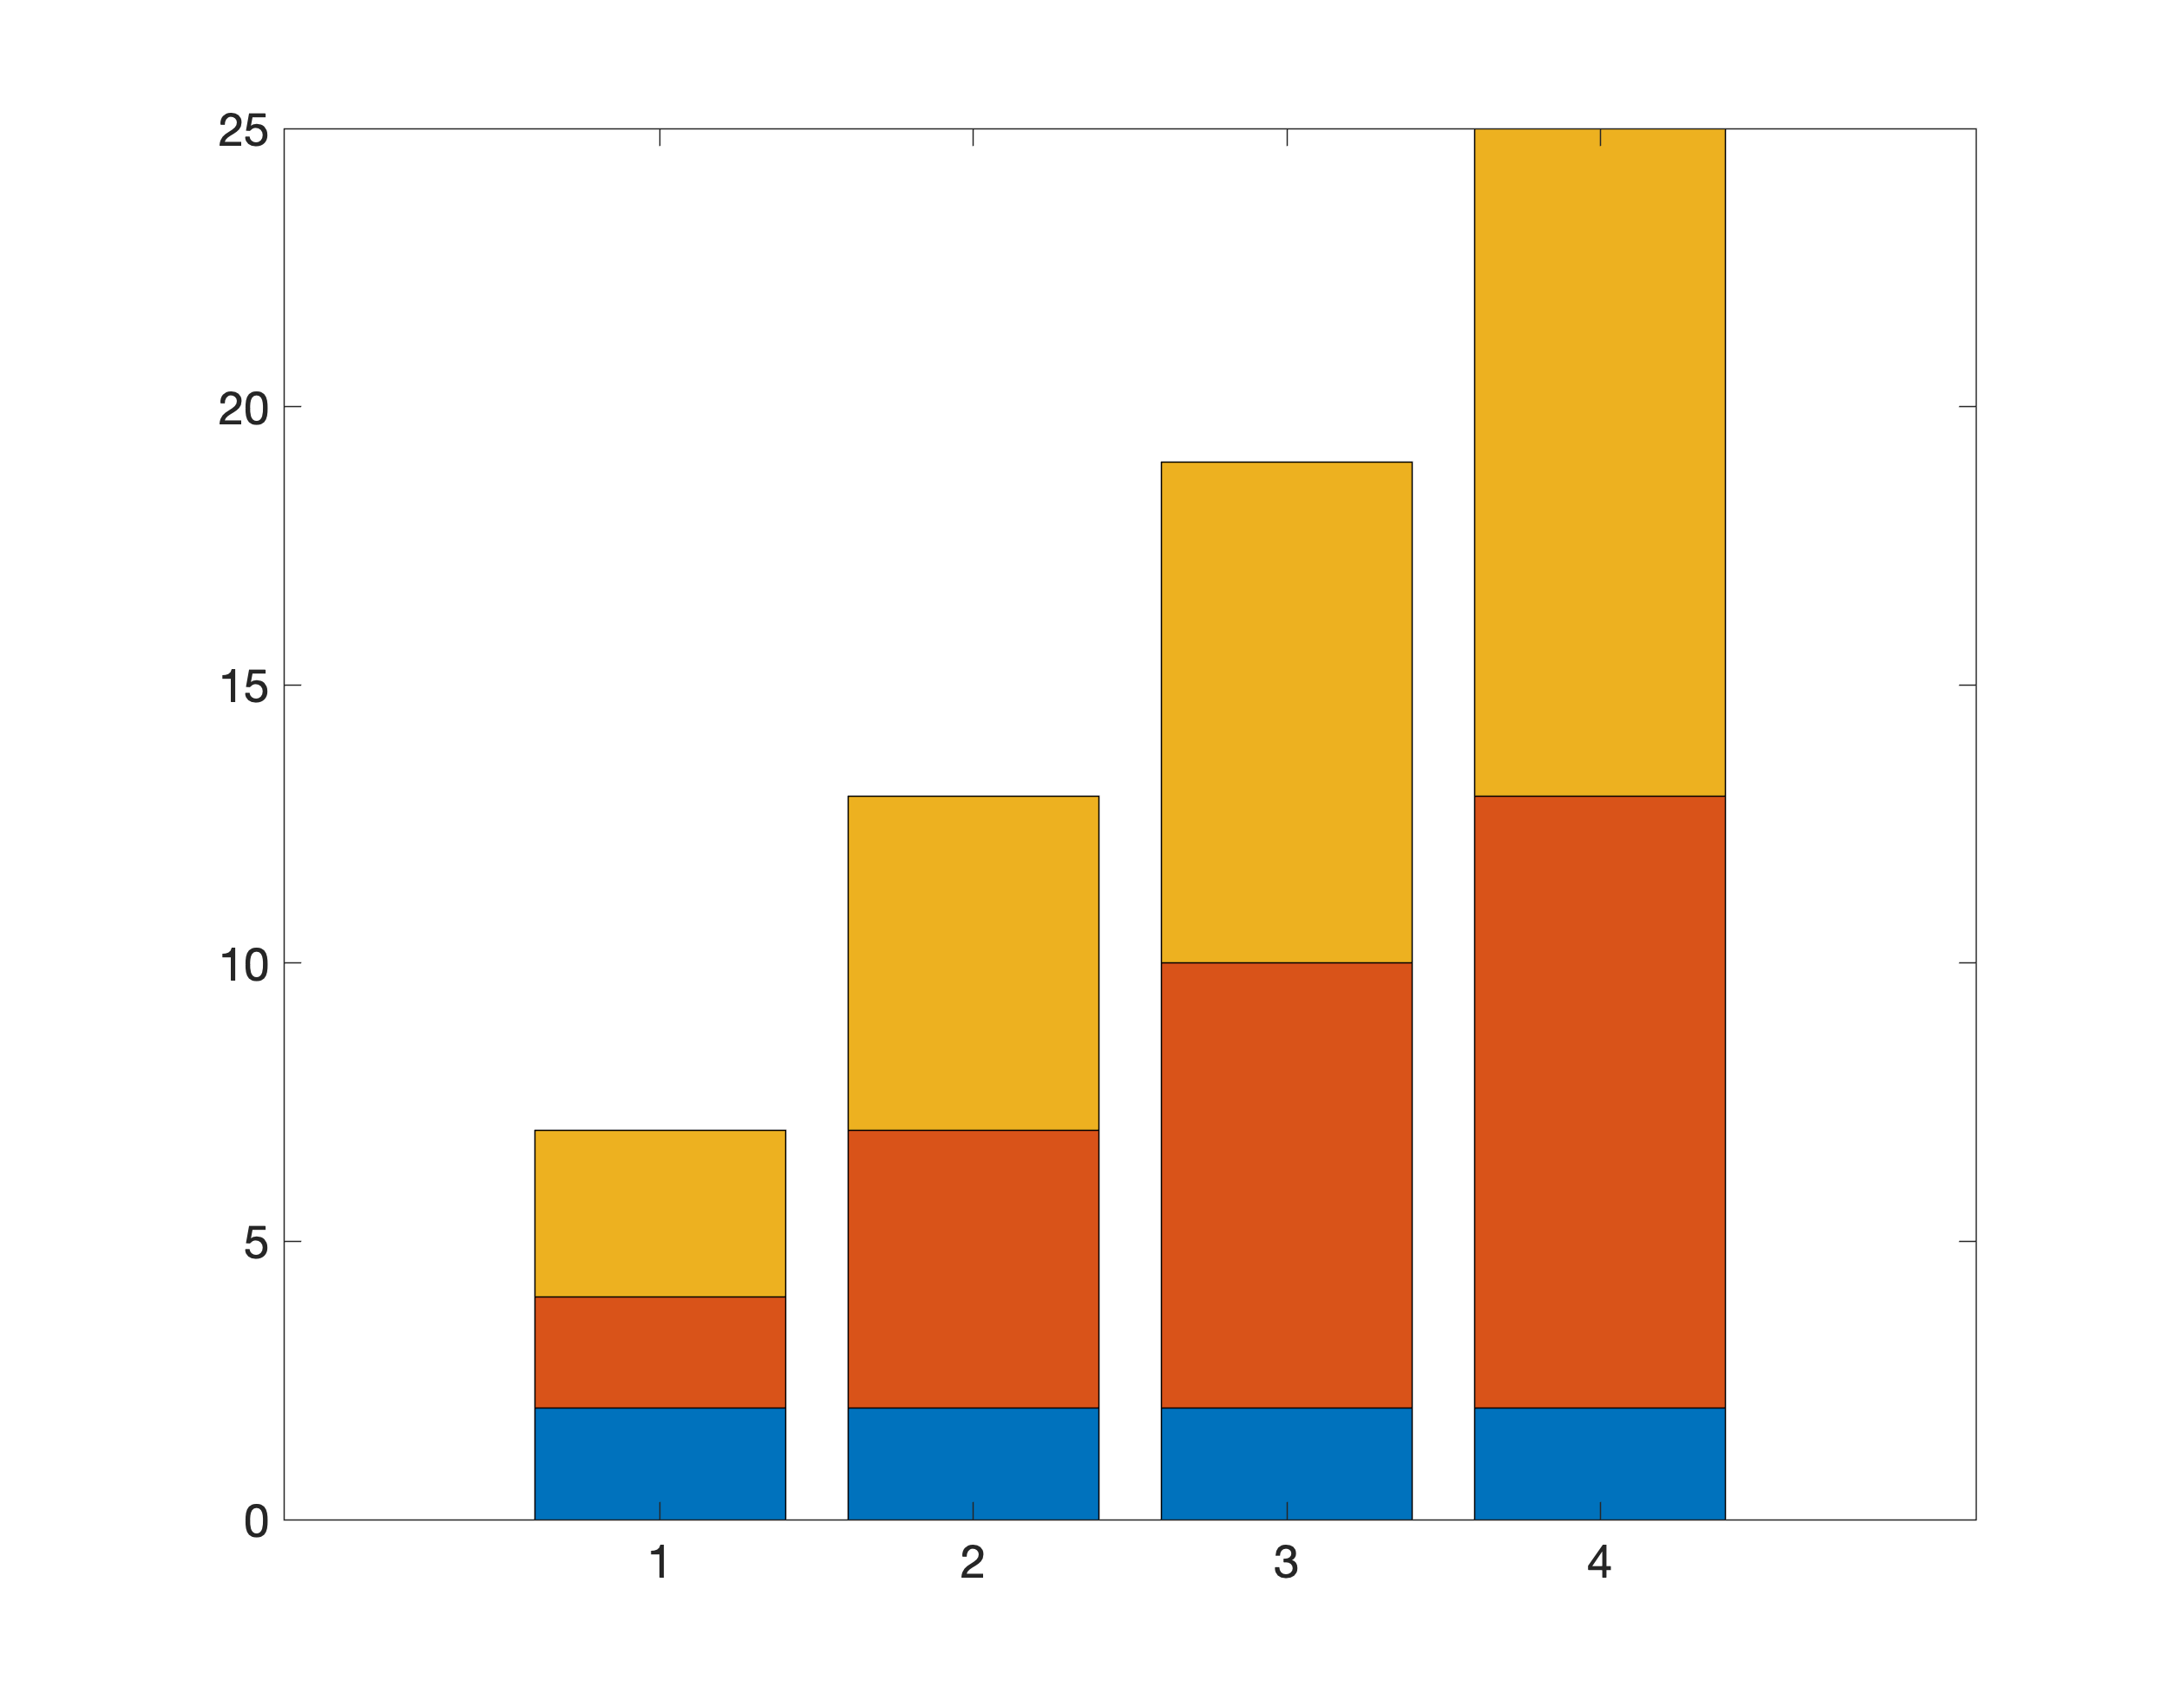
\includegraphics[width=1\linewidth]{./bar_sum.png}
\end{center}
\end{columns}
}

\frame[containsverbatim]
{
\frametitle{Столбчатые диаграммы}
\begin{columns}
\column{.4\textwidth} 
Подписи осей
\begin{lstlisting}
c = categorical({'apples','pears','oranges'});
prices = [1.23 0.99 2.3];
bar(c,prices)
\end{lstlisting}
\column{0.6\textwidth}  
\begin{center}
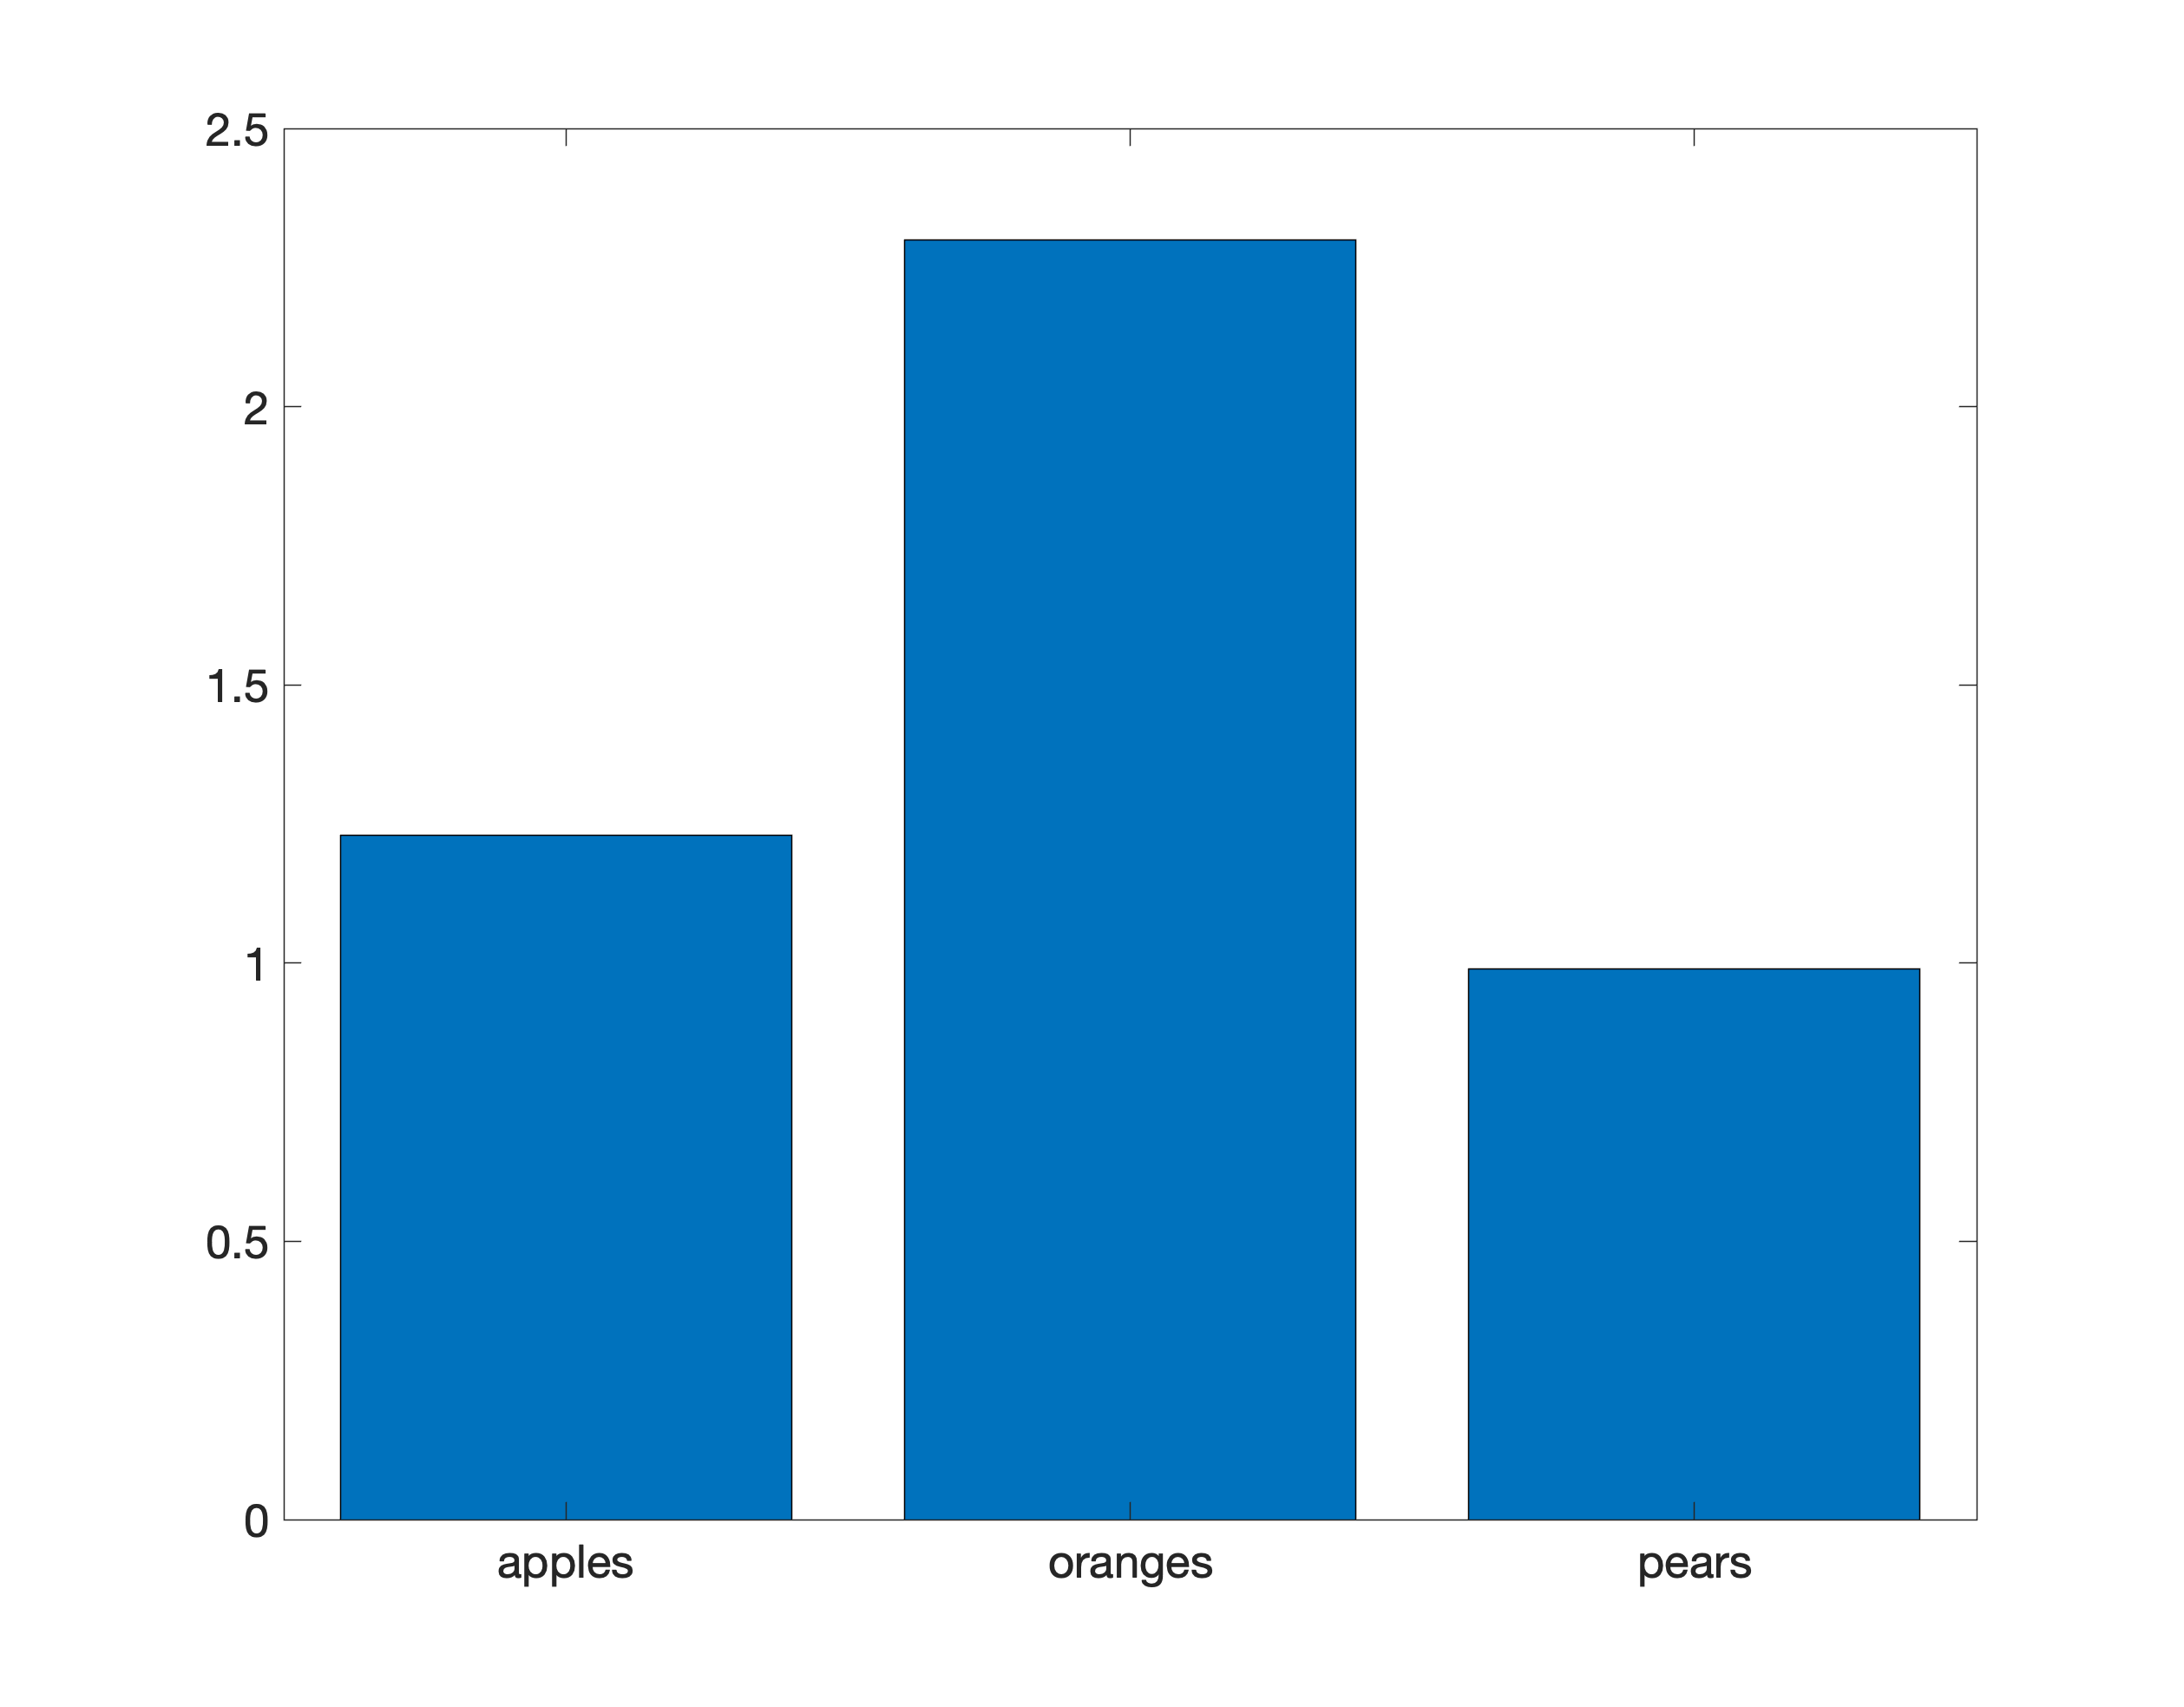
\includegraphics[width=1\linewidth]{./bar_categorical.png}
\end{center}
\end{columns}
}

\frame[containsverbatim]
{
\frametitle{Столбчатые диаграммы}
\begin{columns}
\column{.4\textwidth} 
Цвет
\begin{lstlisting}
y = [75 91 105 123.5];
bar(y,'r')
\end{lstlisting}
\column{0.6\textwidth}  
\begin{center}
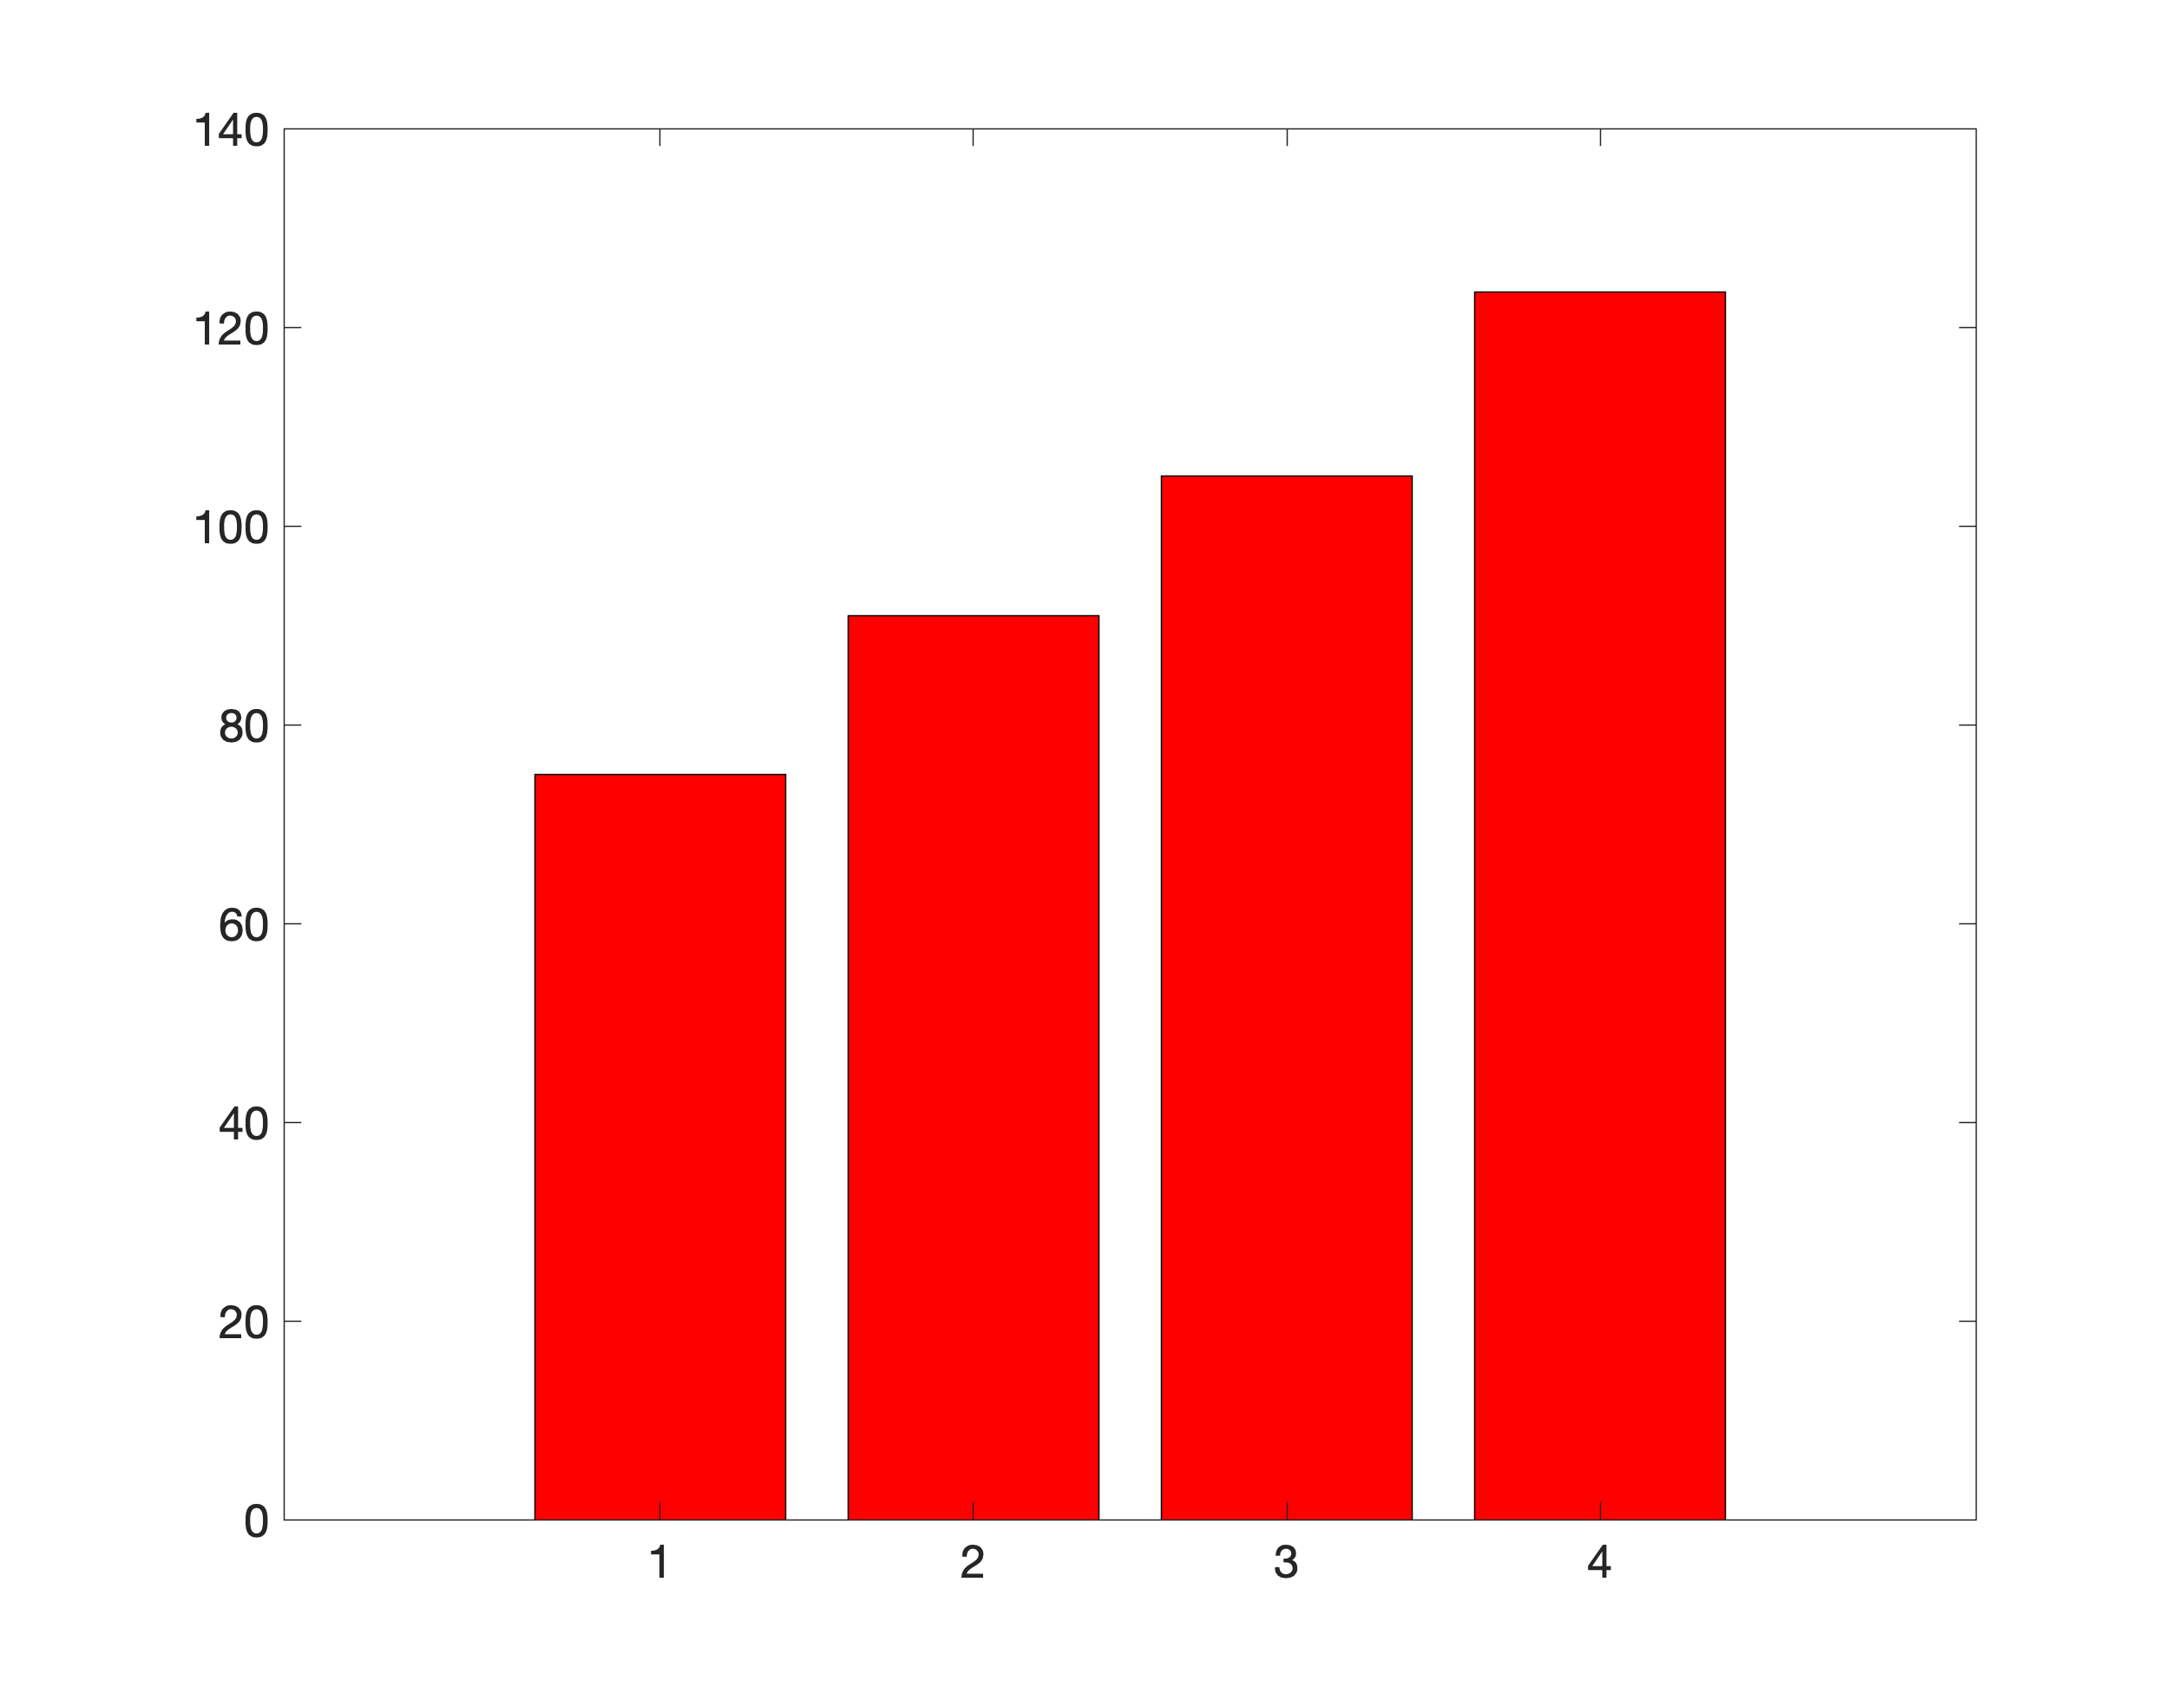
\includegraphics[width=1\linewidth]{./bar_color.png}
\end{center}
\end{columns}
}

\frame[containsverbatim]
{
\frametitle{Столбчатые диаграммы}
\begin{lstlisting}
y = [75 91 105 123.5];
bar(y,'FaceColor',[0.8 0.6 0.6],...
      'EdgeColor',[0.5 0.1 0.1],'LineWidth',3);
\end{lstlisting}
\begin{center}
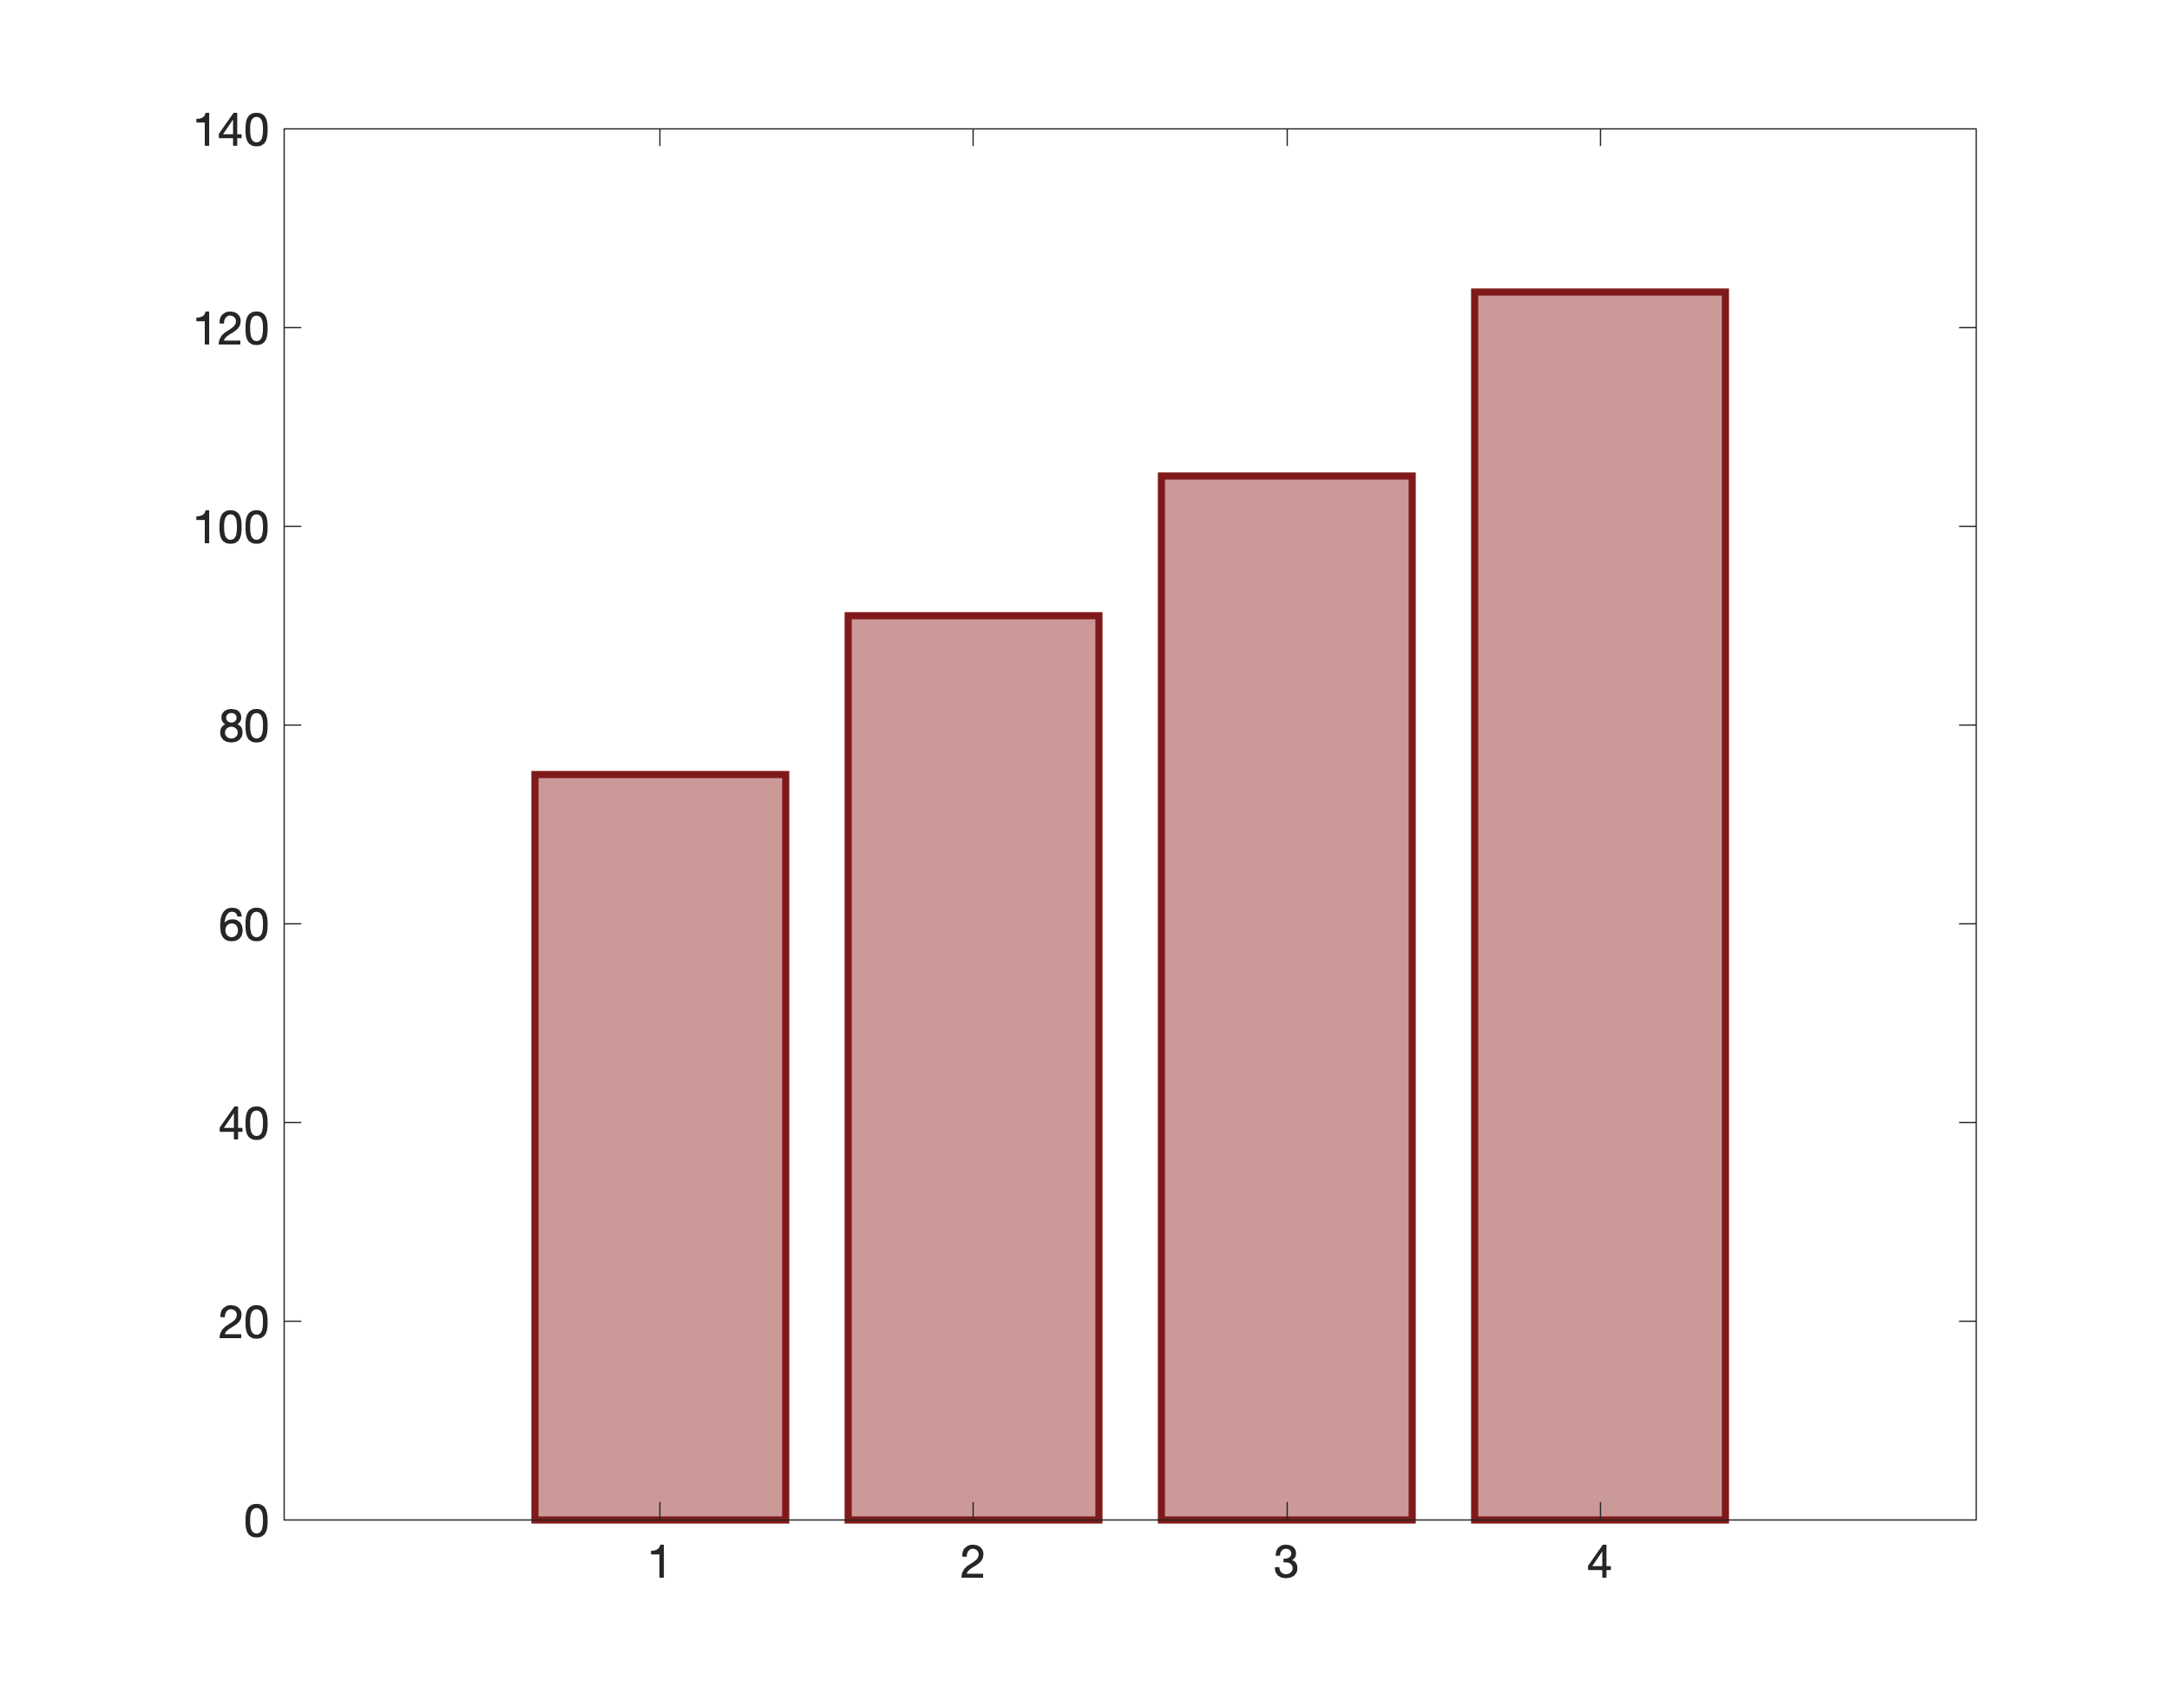
\includegraphics[width=0.7\linewidth]{./bar_color2.png}
\end{center}
}

\frame[containsverbatim]
{
\frametitle{Столбчатые диаграммы}
\begin{columns}
\column{.4\textwidth} 
Изменение цвета отдельных столбцов
\begin{lstlisting}
y = [75 91 105 123.5];
b = bar(y);
b.FaceColor = 'flat';
b.CData(2,:) = [1 0 0];
\end{lstlisting}
\column{0.6\textwidth}  
\begin{center}
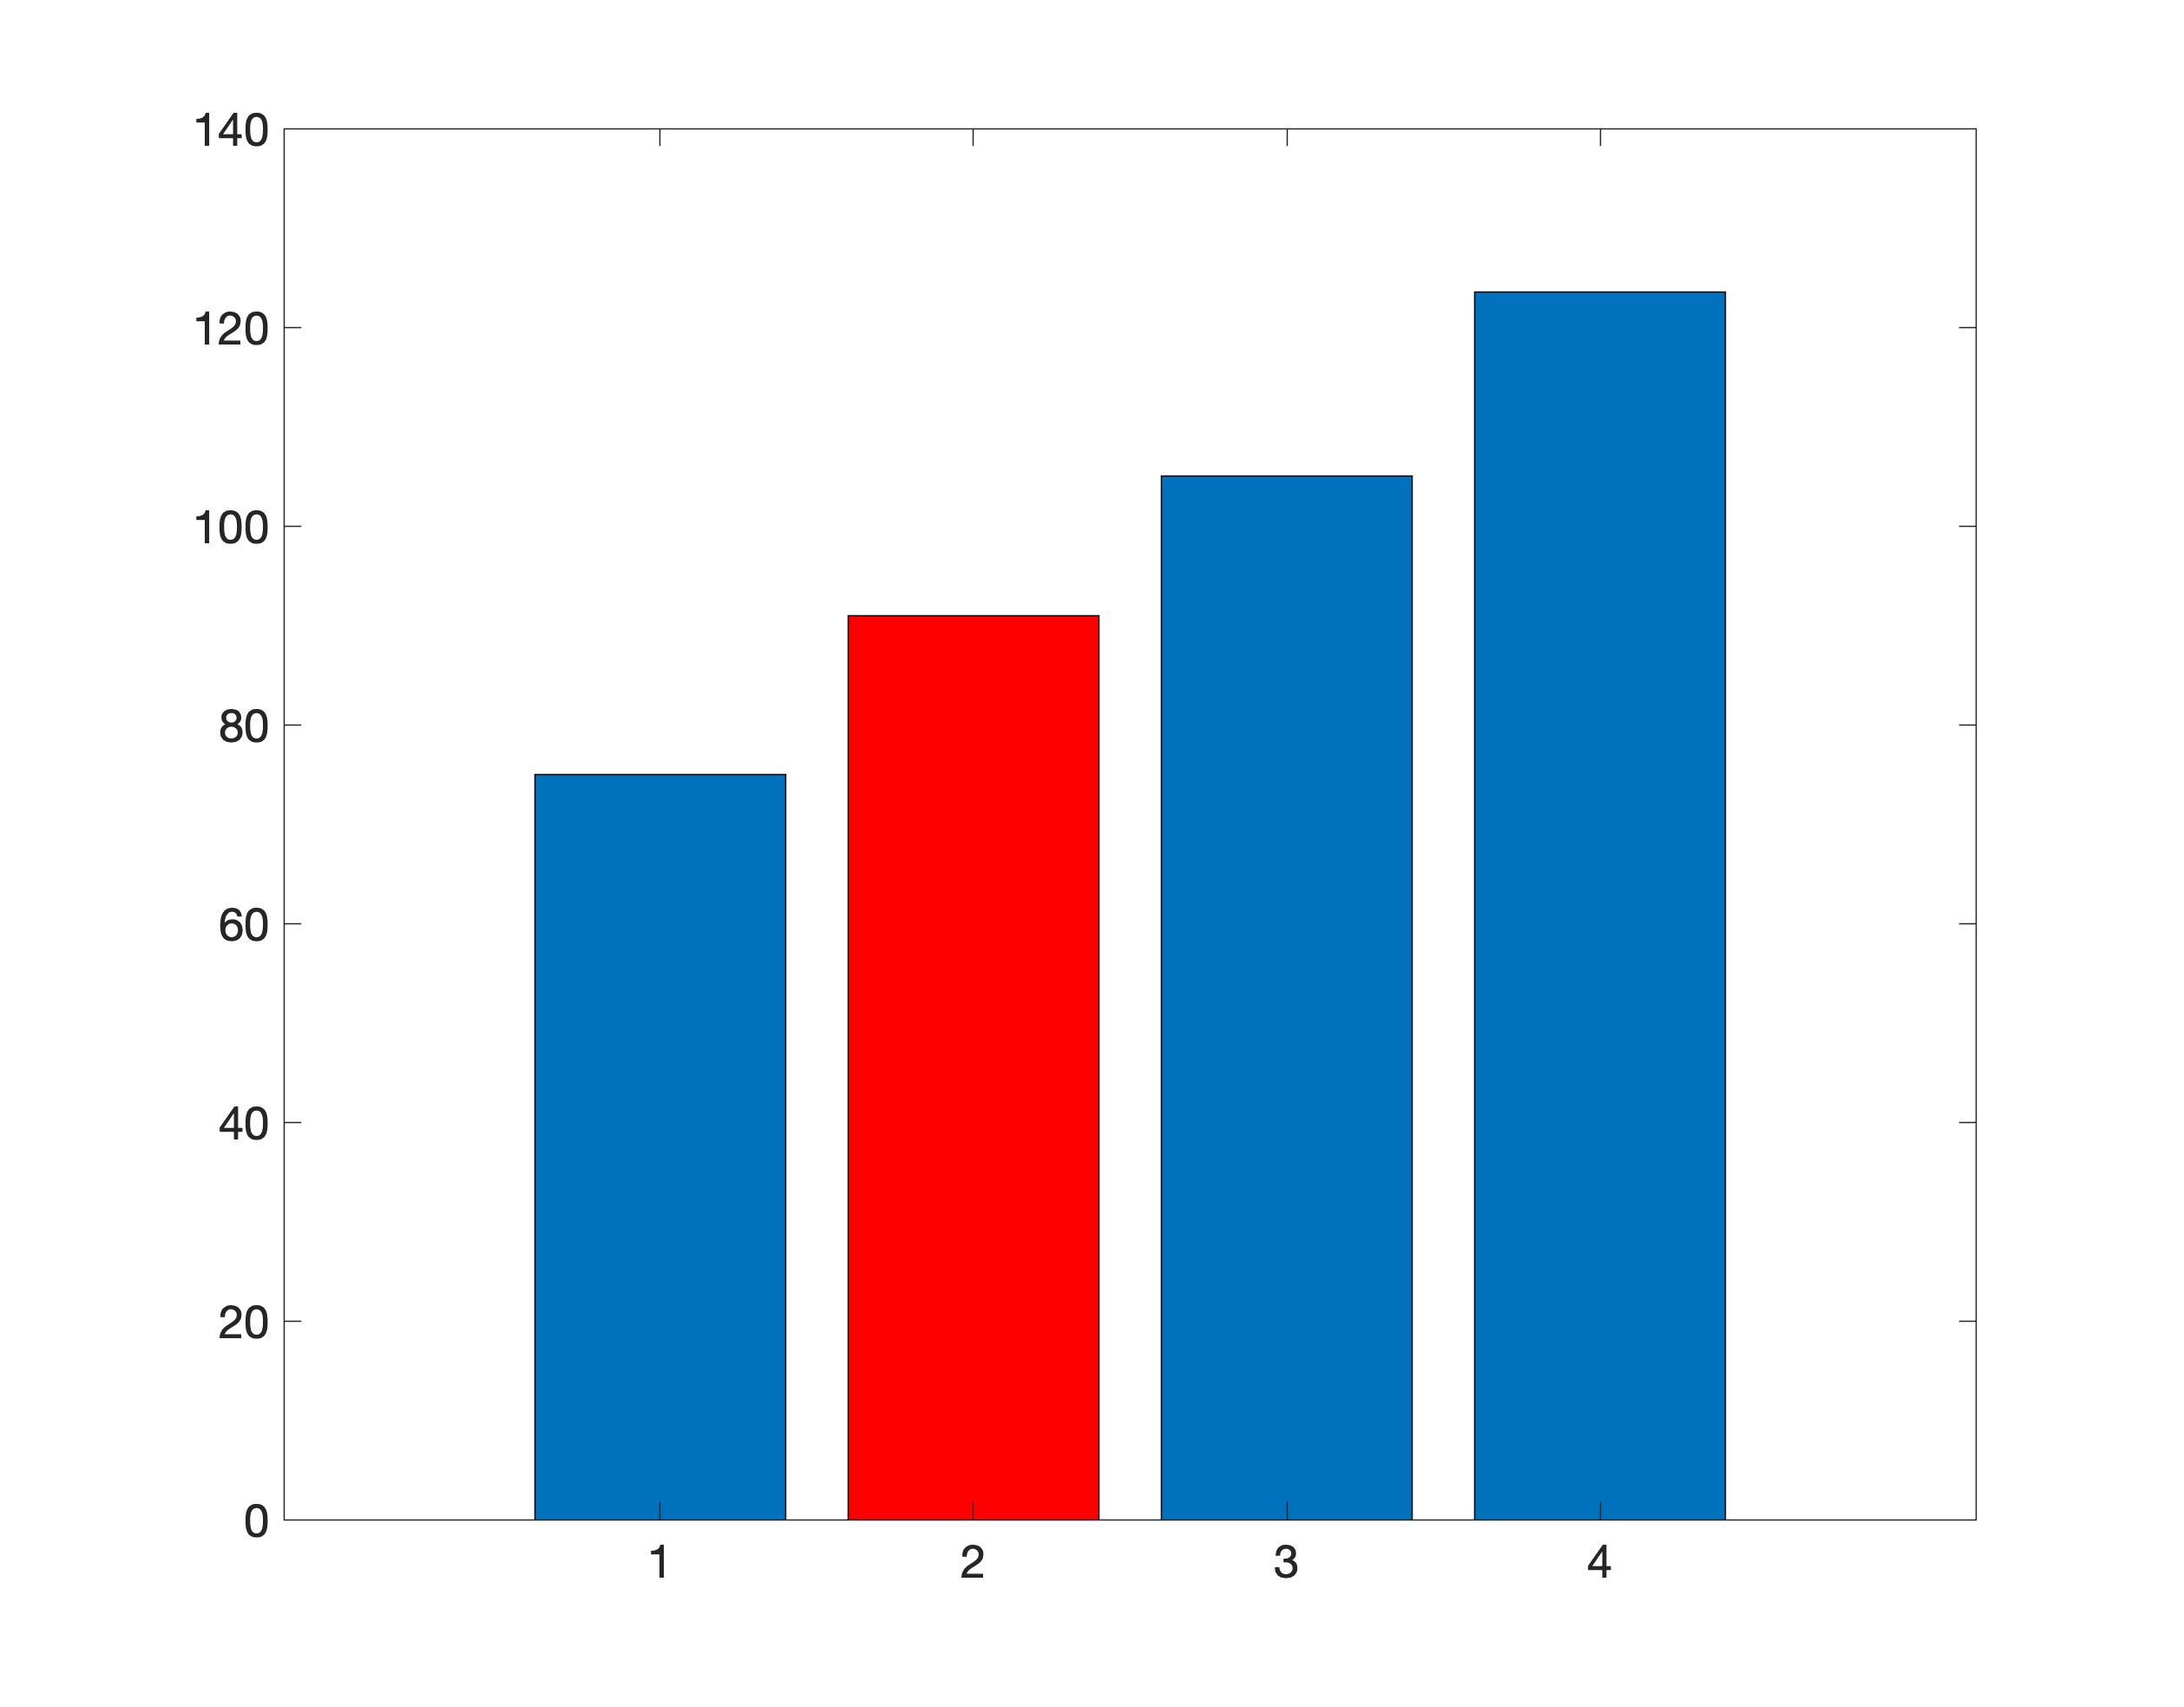
\includegraphics[width=1\linewidth]{./bar_color3.png}
\end{center}
\end{columns}
}



\frame[containsverbatim]
{
\frametitle{Круговые диаграммы}
\begin{columns}
\column{.4\textwidth}
\begin{lstlisting}
x=[1,2,3,4];
pie(x)
\end{lstlisting}
Второй аргумент -- логический массив, указывающий на необходимость изображения соответствующего сектора отдельно от круговой диаграммы
\begin{lstlisting}
y=[0,0,1,0];
pie(x,y)
\end{lstlisting}
\column{0.6\textwidth}
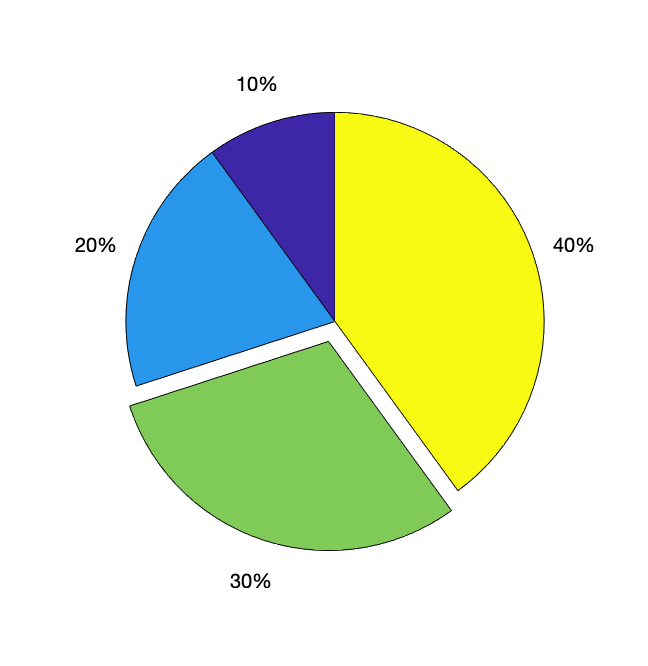
\includegraphics[width=1\linewidth]{./pie.png}
\end{columns}
}

\frame[containsverbatim]
{
\frametitle{Круговые диаграммы}
Если сумма элементов массива данных больше или равна единице, то эта сумма принимается за 100\%, в противном случае строится диаграмма с пропущенным сектором.
\begin{columns}
\column{.5\textwidth}
\begin{lstlisting}
x=[0.1,0.2,0.5];
pie(x)
\end{lstlisting}  
\column{.5\textwidth}
\begin{center}
 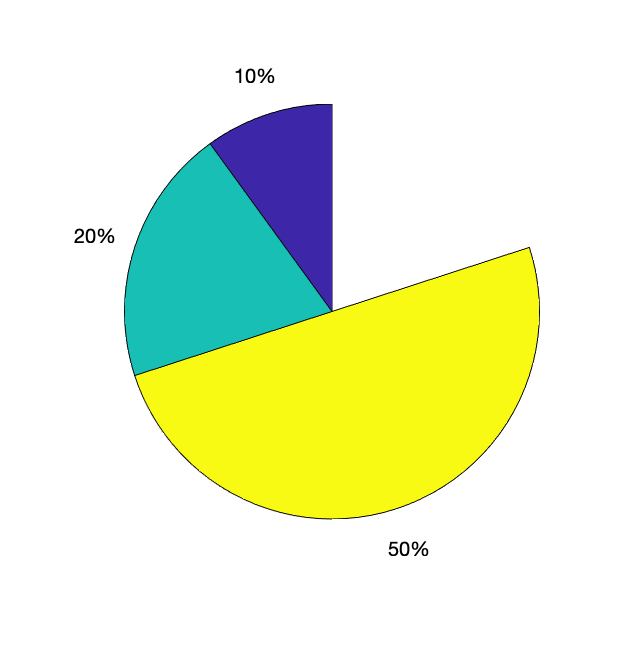
\includegraphics[width=1\linewidth]{./pie-sec.png}
\end{center}  
\end{columns}
}


\frame[containsverbatim]
{
\frametitle{Круговые диаграммы}
\begin{lstlisting}
X = 1:3;
labels = {'Taxes','Expenses','Profit'};
hp = pie(X,labels)

>> hp
  1×6 graphics array:

    Patch    Text     Patch    Text     Patch    Text 
\end{lstlisting}
}


\frame[containsverbatim]
{
\frametitle{Круговые диаграммы}
\begin{lstlisting}
set(hp(2:2:6),'FontSize',18);
\end{lstlisting}
или
\begin{lstlisting}
set(findobj(hp,'type','text'),'FontSize',18);
\end{lstlisting}
\begin{center}
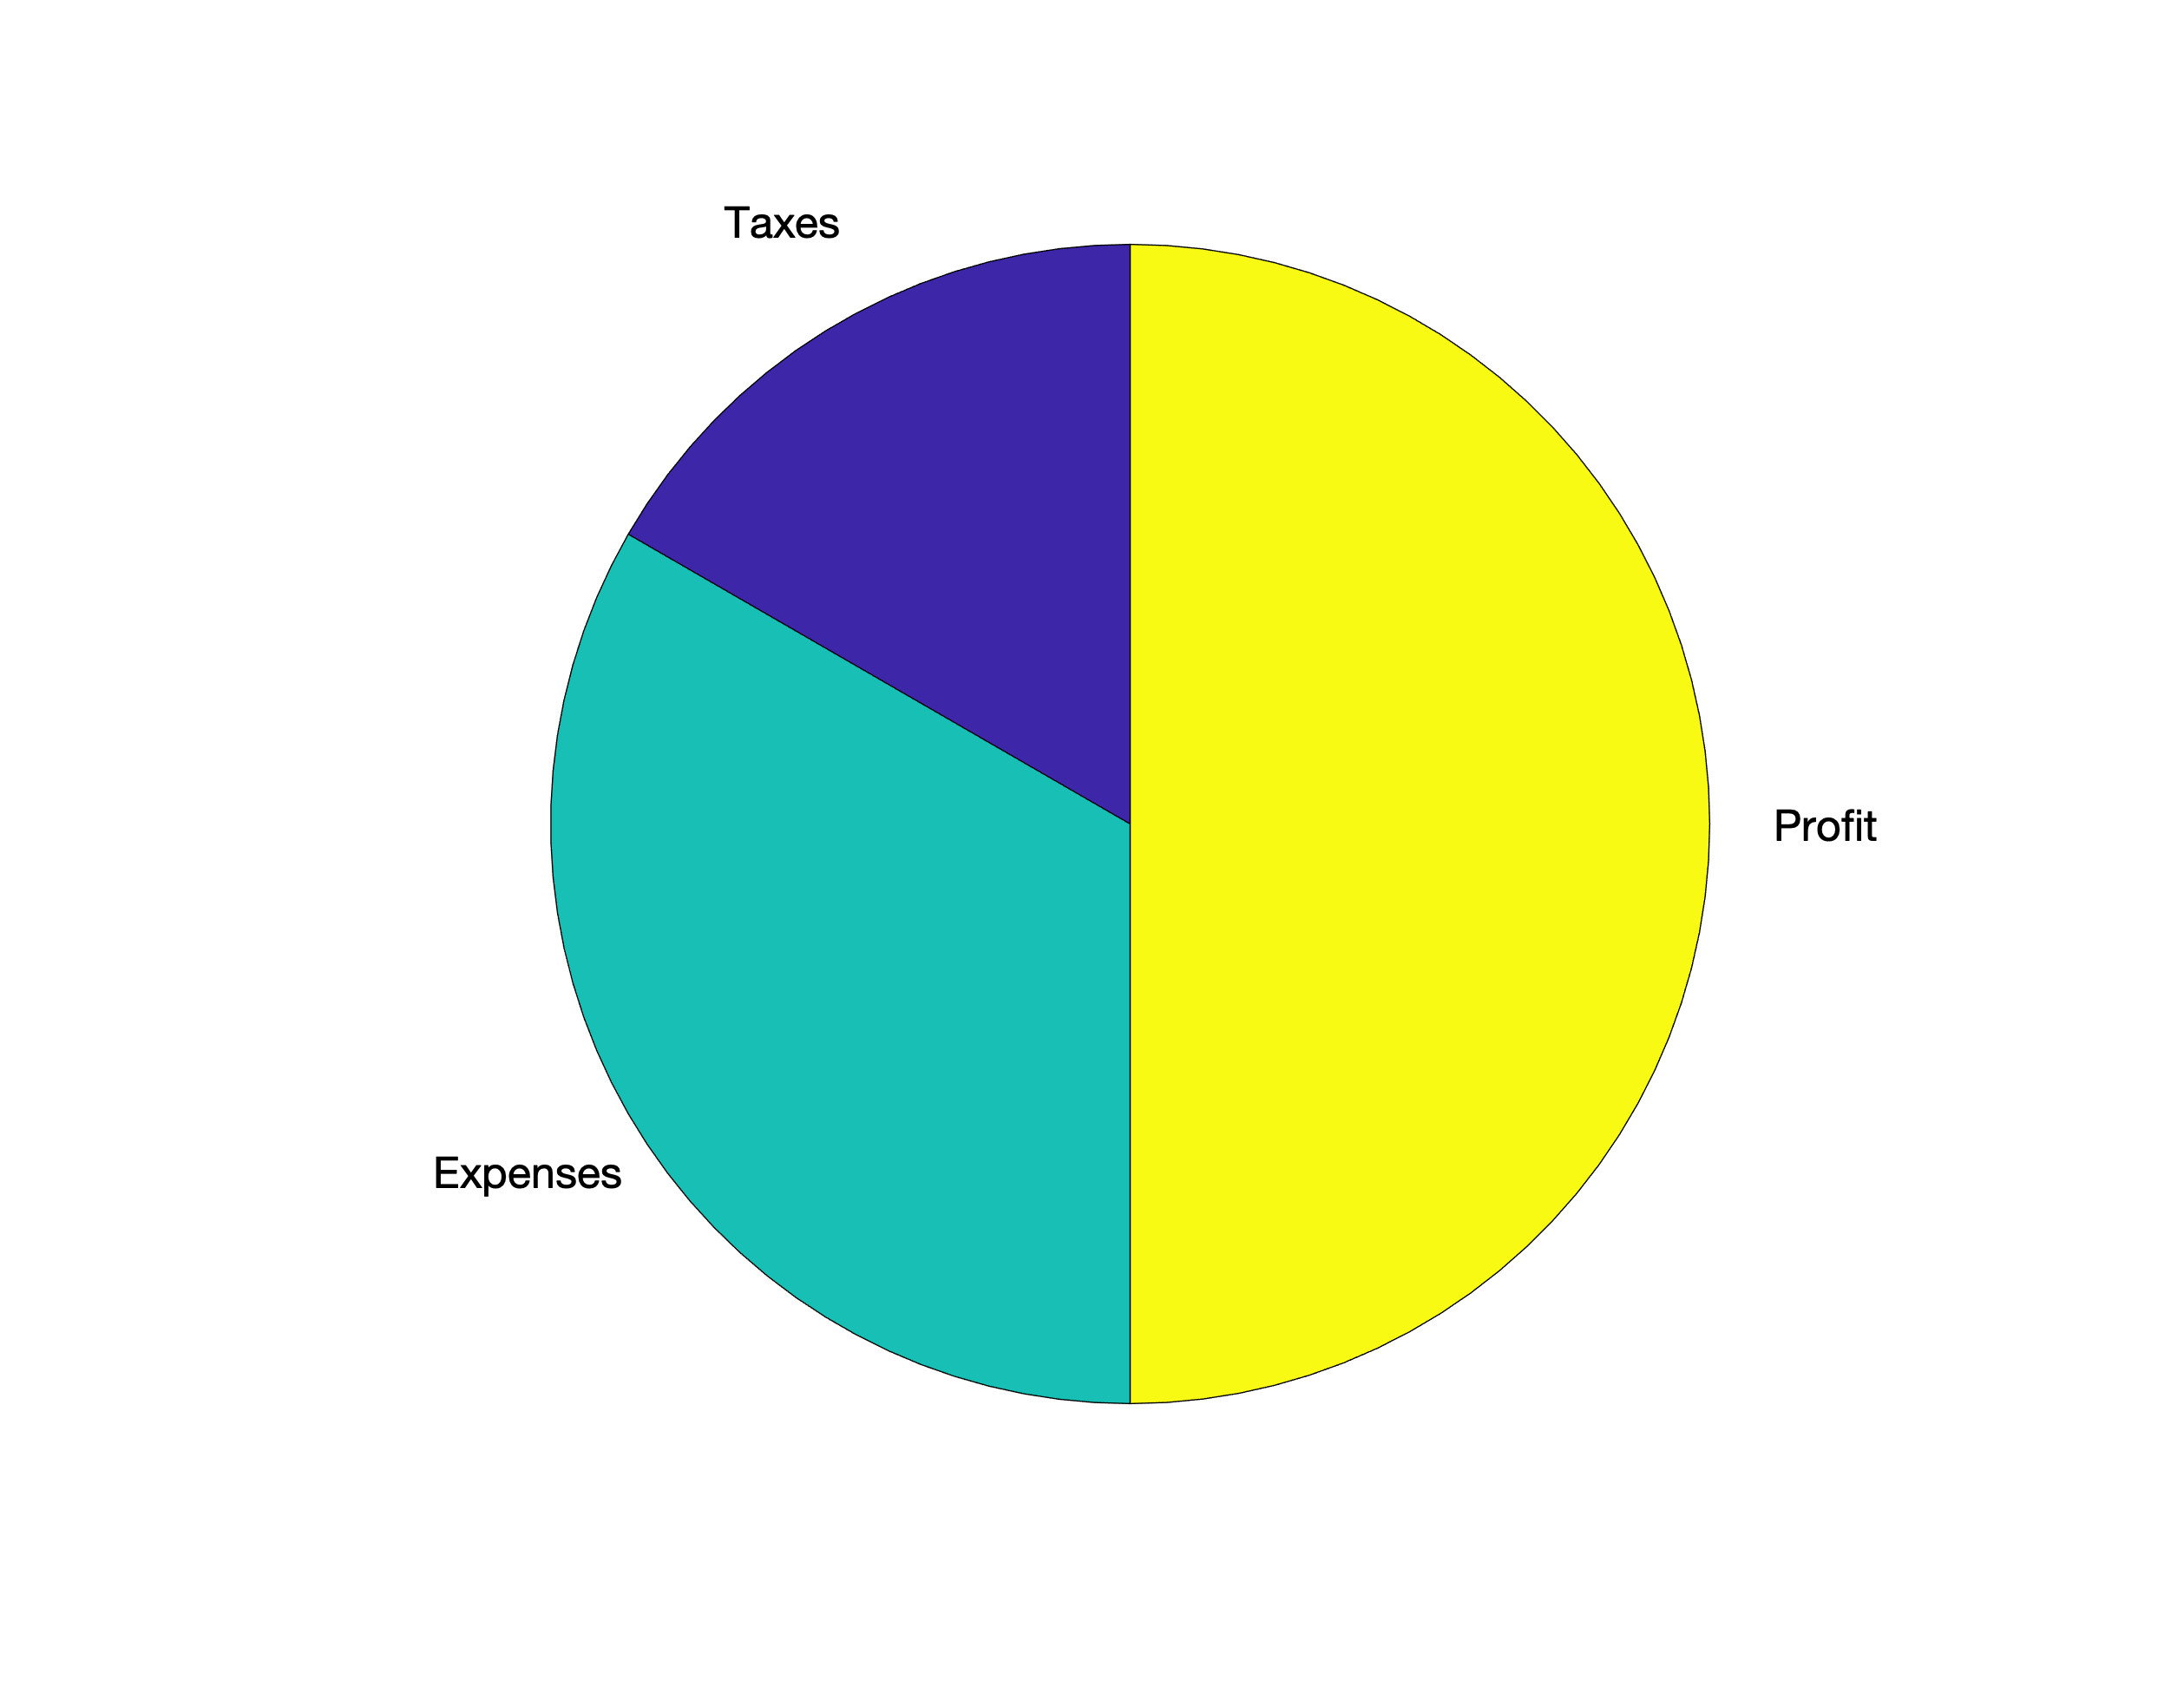
\includegraphics[width=0.7\linewidth]{./pie_text.png}
\end{center}
}

\frame[containsverbatim]
{
\frametitle{Гистограммы}
\begin{columns}
\column{.5\textwidth}
Вектор-строка 90 случайных чисел, распределённых по нормальному закону с $m=0$ и $\sigma = 2$ 
\begin{lstlisting}
y=random('norm',0,2,1,90);
\end{lstlisting}
Функция \matcode{hist} делит интервал $y$ на 10 частей и строит гистограмму:
\begin{lstlisting}
hist(y)
\end{lstlisting}
\column{.5\textwidth}
\begin{center}
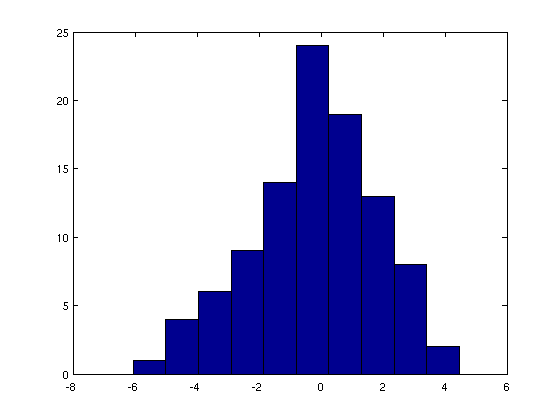
\includegraphics[width=1\linewidth]{./hist.png}
\end{center}  
\end{columns}
}

\frame[containsverbatim]
{
\frametitle{Круговая гистограмма}
\begin{columns}
\column{.5\textwidth}
Генерируем вектор-строку 90 случайных чисел, распределённых по нормальному закону с $m=0$ и $\sigma = 1$
\begin{lstlisting}
y=random('norm',0,1,1,90); 
\end{lstlisting}
Функция \matcode{rose} строит гистограмму в полярных координатах, предполагая, что элементы массива \matcode{y} заданы в радианах.
\begin{lstlisting}
rose(y)
\end{lstlisting}
\column{.5\textwidth}
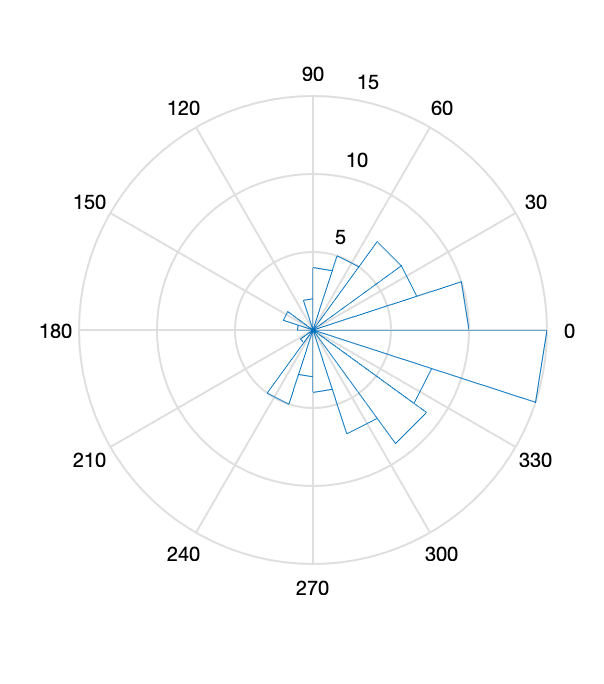
\includegraphics[width=1\linewidth]{./rose.png}
\end{columns}
}

\begin{frame}[c,fragile]
\frametitle{area}
\begin{columns}
\column{.5\textwidth}
\begin{lstlisting}
Y = [1, 5, 3];
area(Y);    
\end{lstlisting}
\column{.5\textwidth}
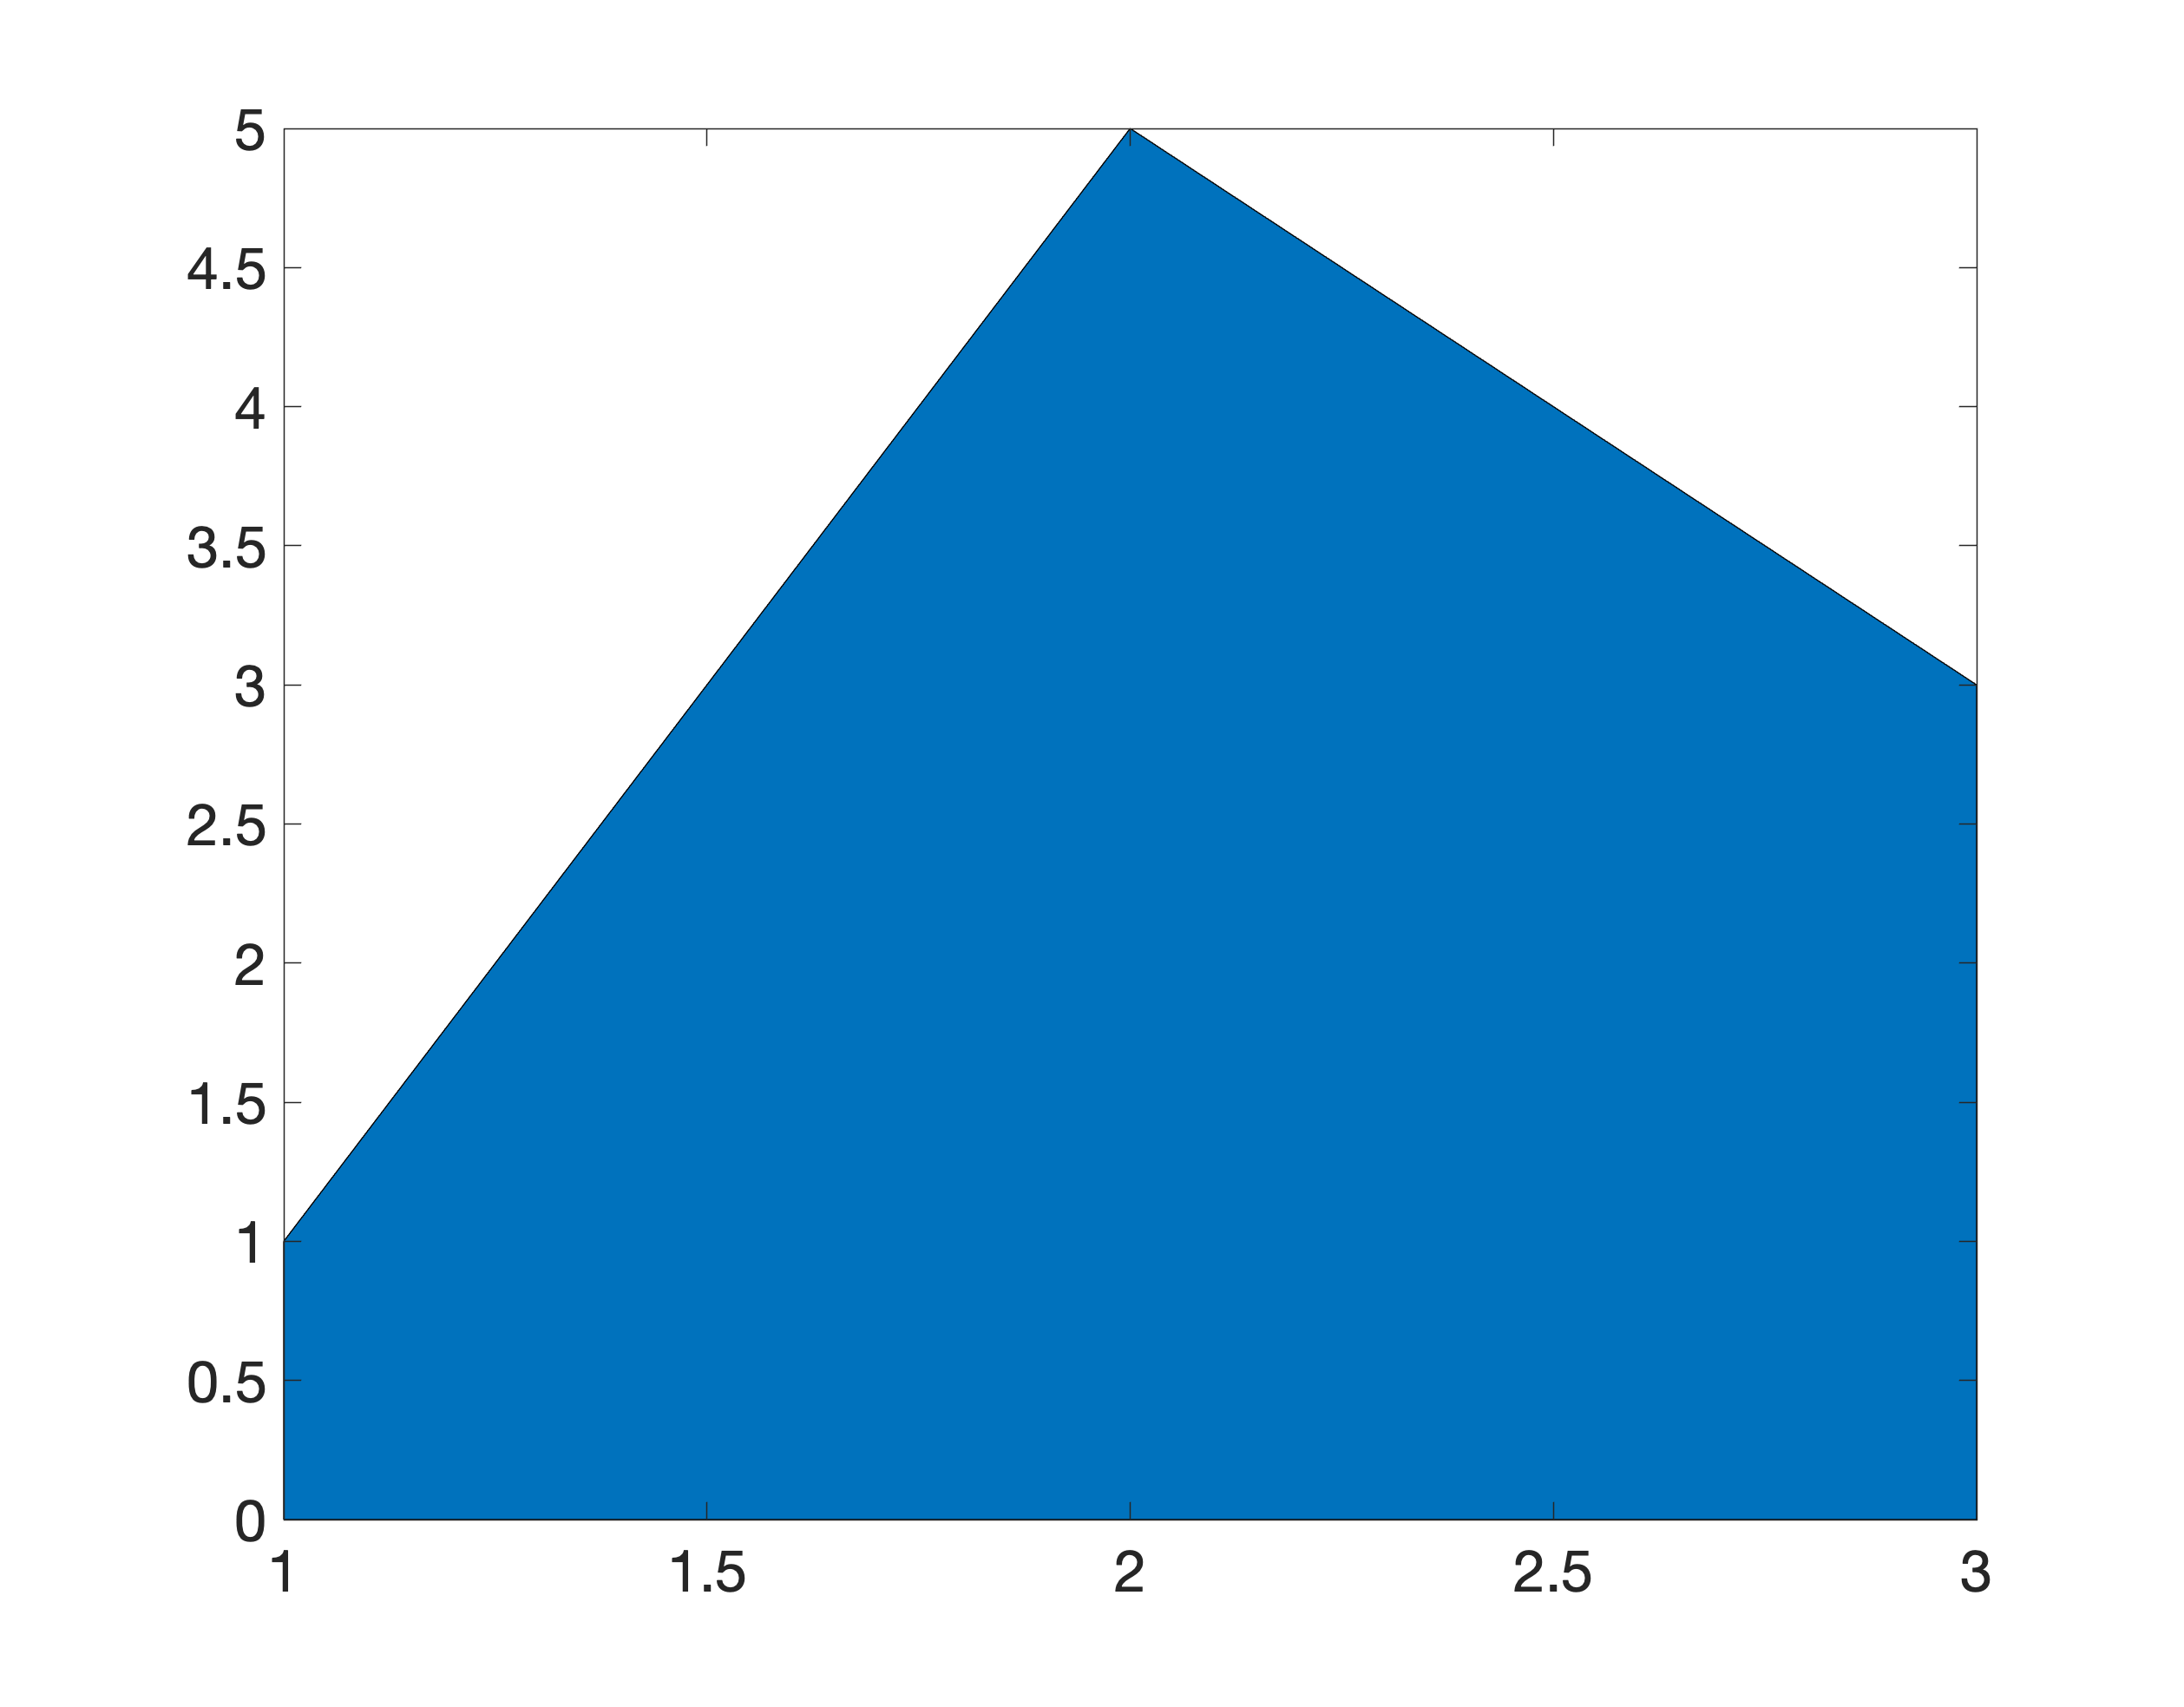
\includegraphics[width=1\linewidth]{./area.png}
\end{columns}
\end{frame}

\begin{frame}[c,fragile]
\frametitle{area}
\begin{columns}
\column{.5\textwidth}
\begin{lstlisting}
Y = [1, 5, 3;
     3, 2, 7;
     1, 5, 3;
     2, 6, 1];
area(Y);  
\end{lstlisting}
\column{.5\textwidth}
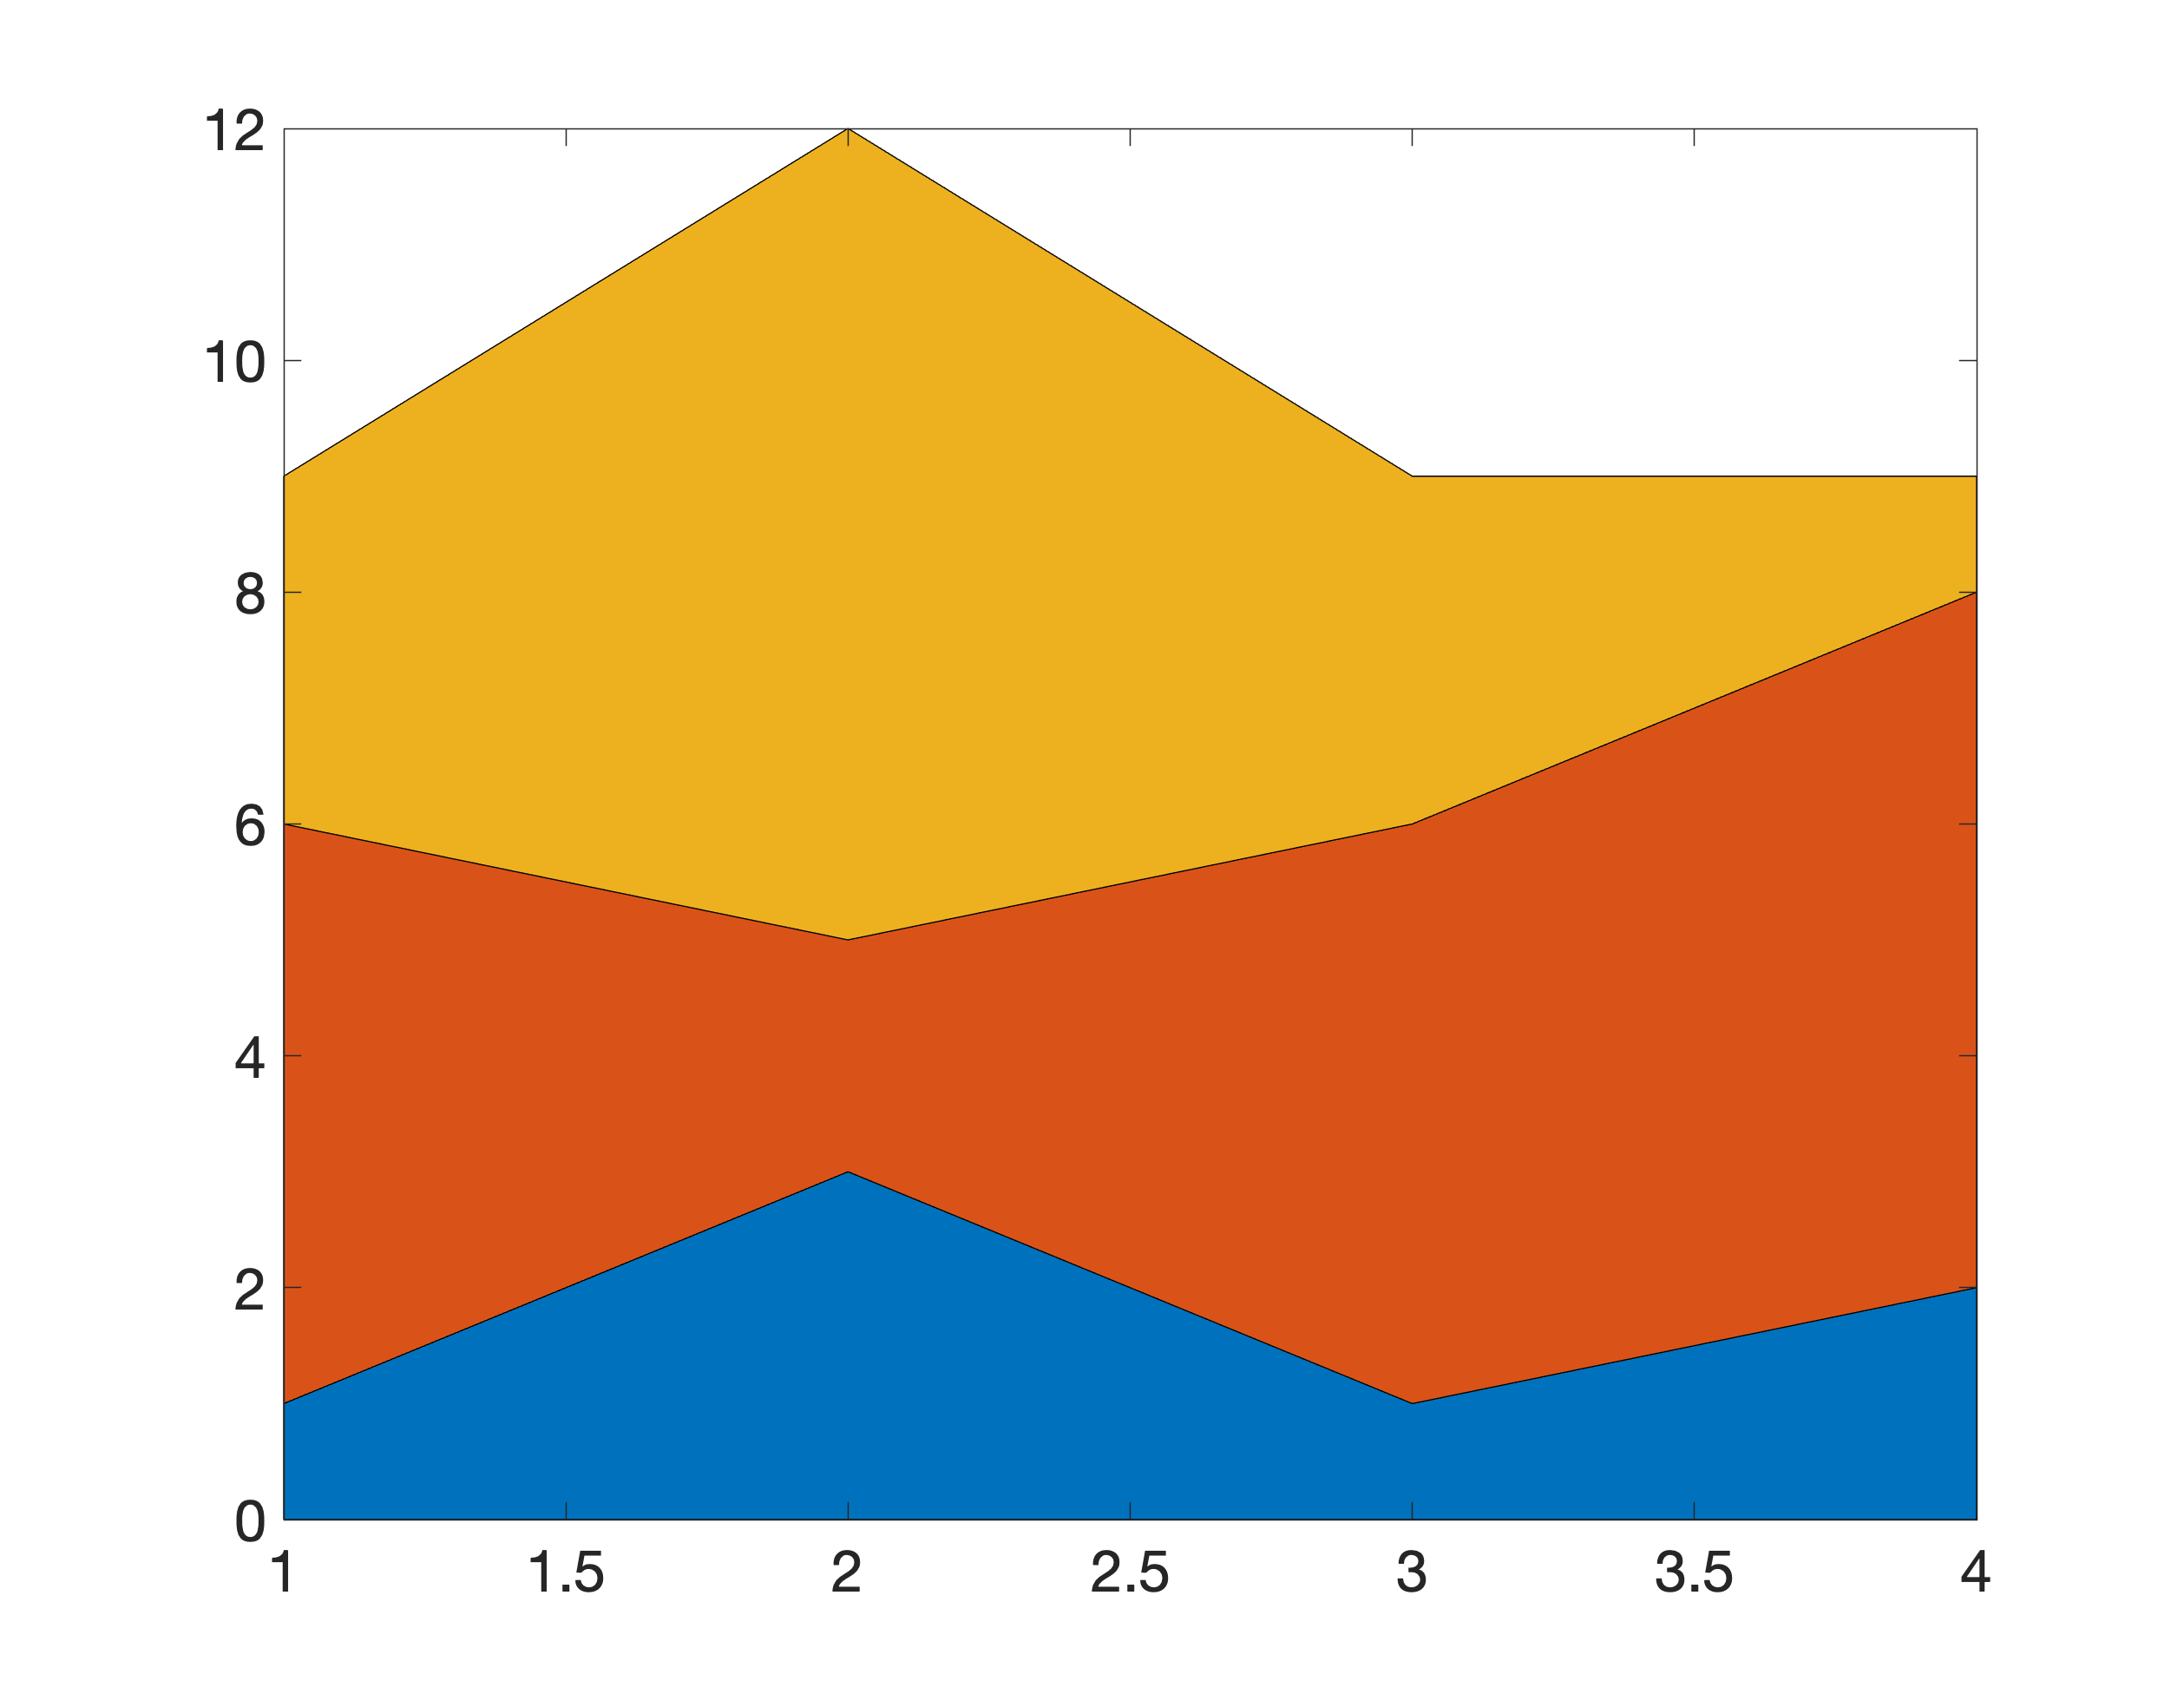
\includegraphics[width=1\linewidth]{./area2.png}
\end{columns}
\end{frame}

\begin{frame}[c,fragile]
\frametitle{График с оценкой погрешности}
\begin{columns}
\column{.5\textwidth}
\begin{lstlisting}
x = 0:10:40;
y = [20 30 45 40 60];
err = [1 3 5 3 5];
errorbar(x,y,err,...
'LineWidth',2); 
\end{lstlisting}
\column{.5\textwidth}
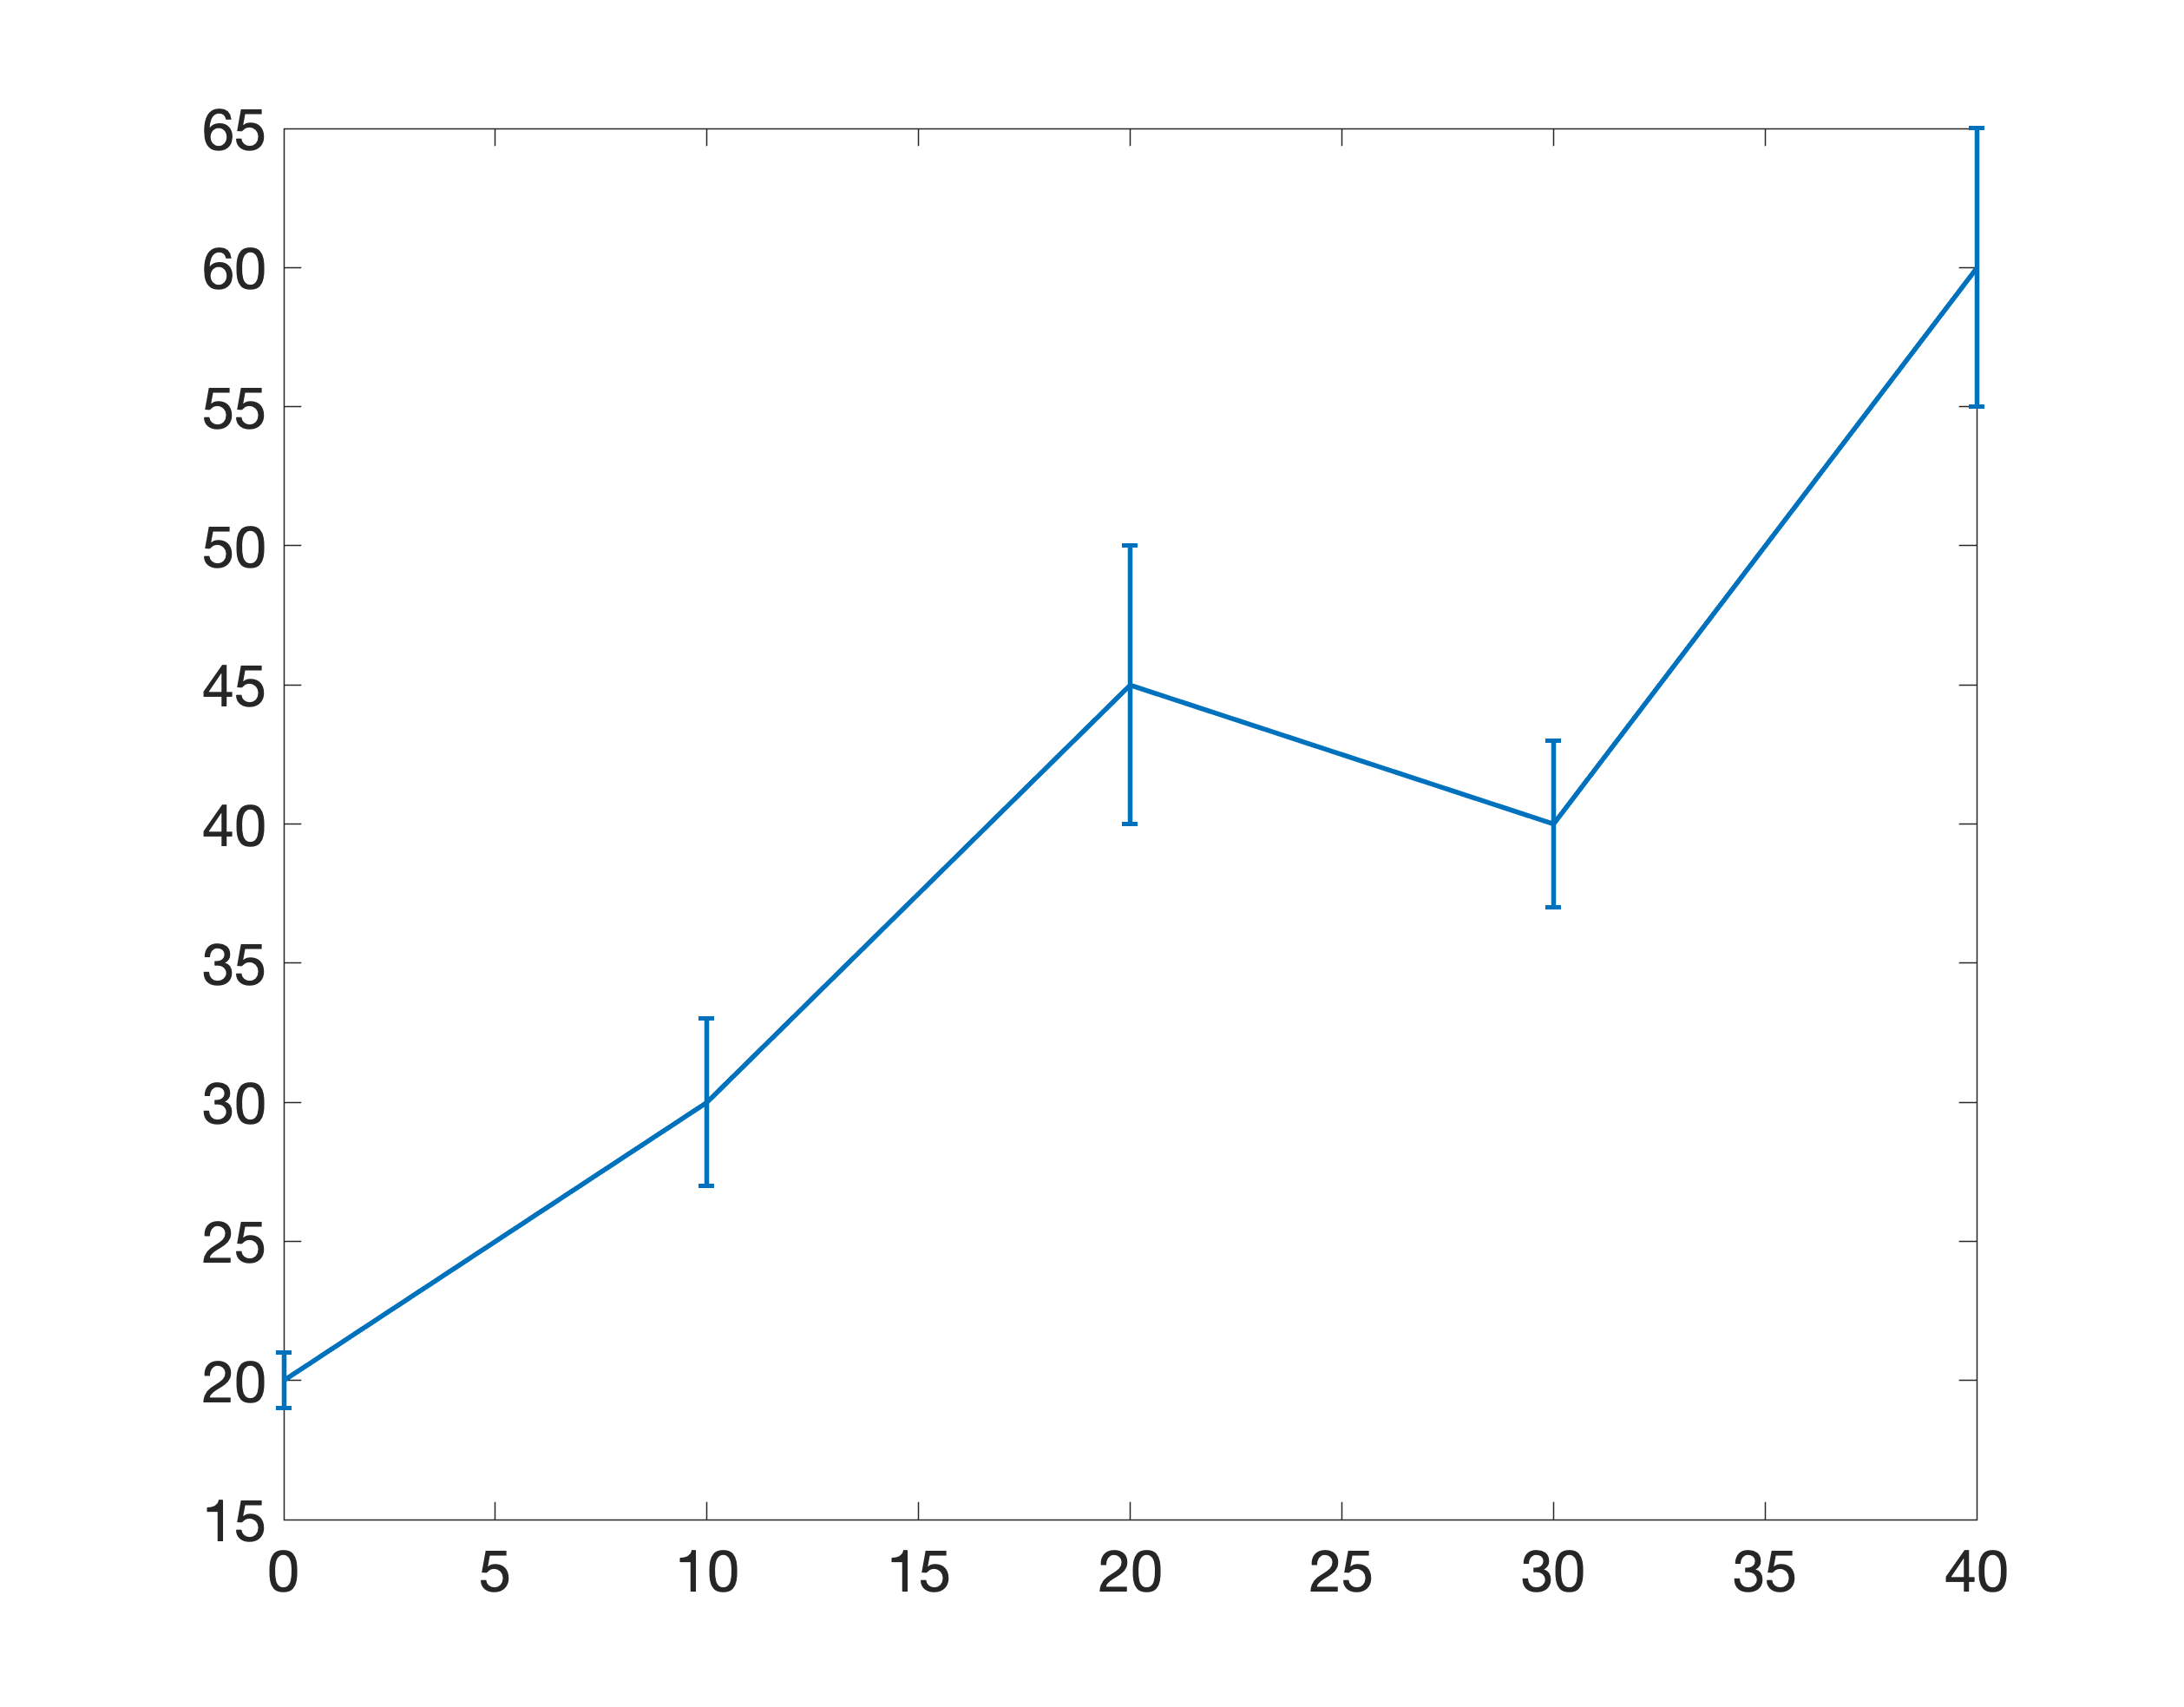
\includegraphics[width=1\linewidth]{./error.png}
\end{columns}    
\end{frame}

\begin{frame}[c,fragile]
\frametitle{График с оценкой погрешности}
\begin{columns}
\column{.5\textwidth}
\begin{lstlisting}
x = 0:10:40;
y = [20 30 45 40 60];
err = [1 3 5 3 5];
errorbar(x,y,err,...
'horizontal',...
'LineWidth',2);
\end{lstlisting}
\column{.5\textwidth}
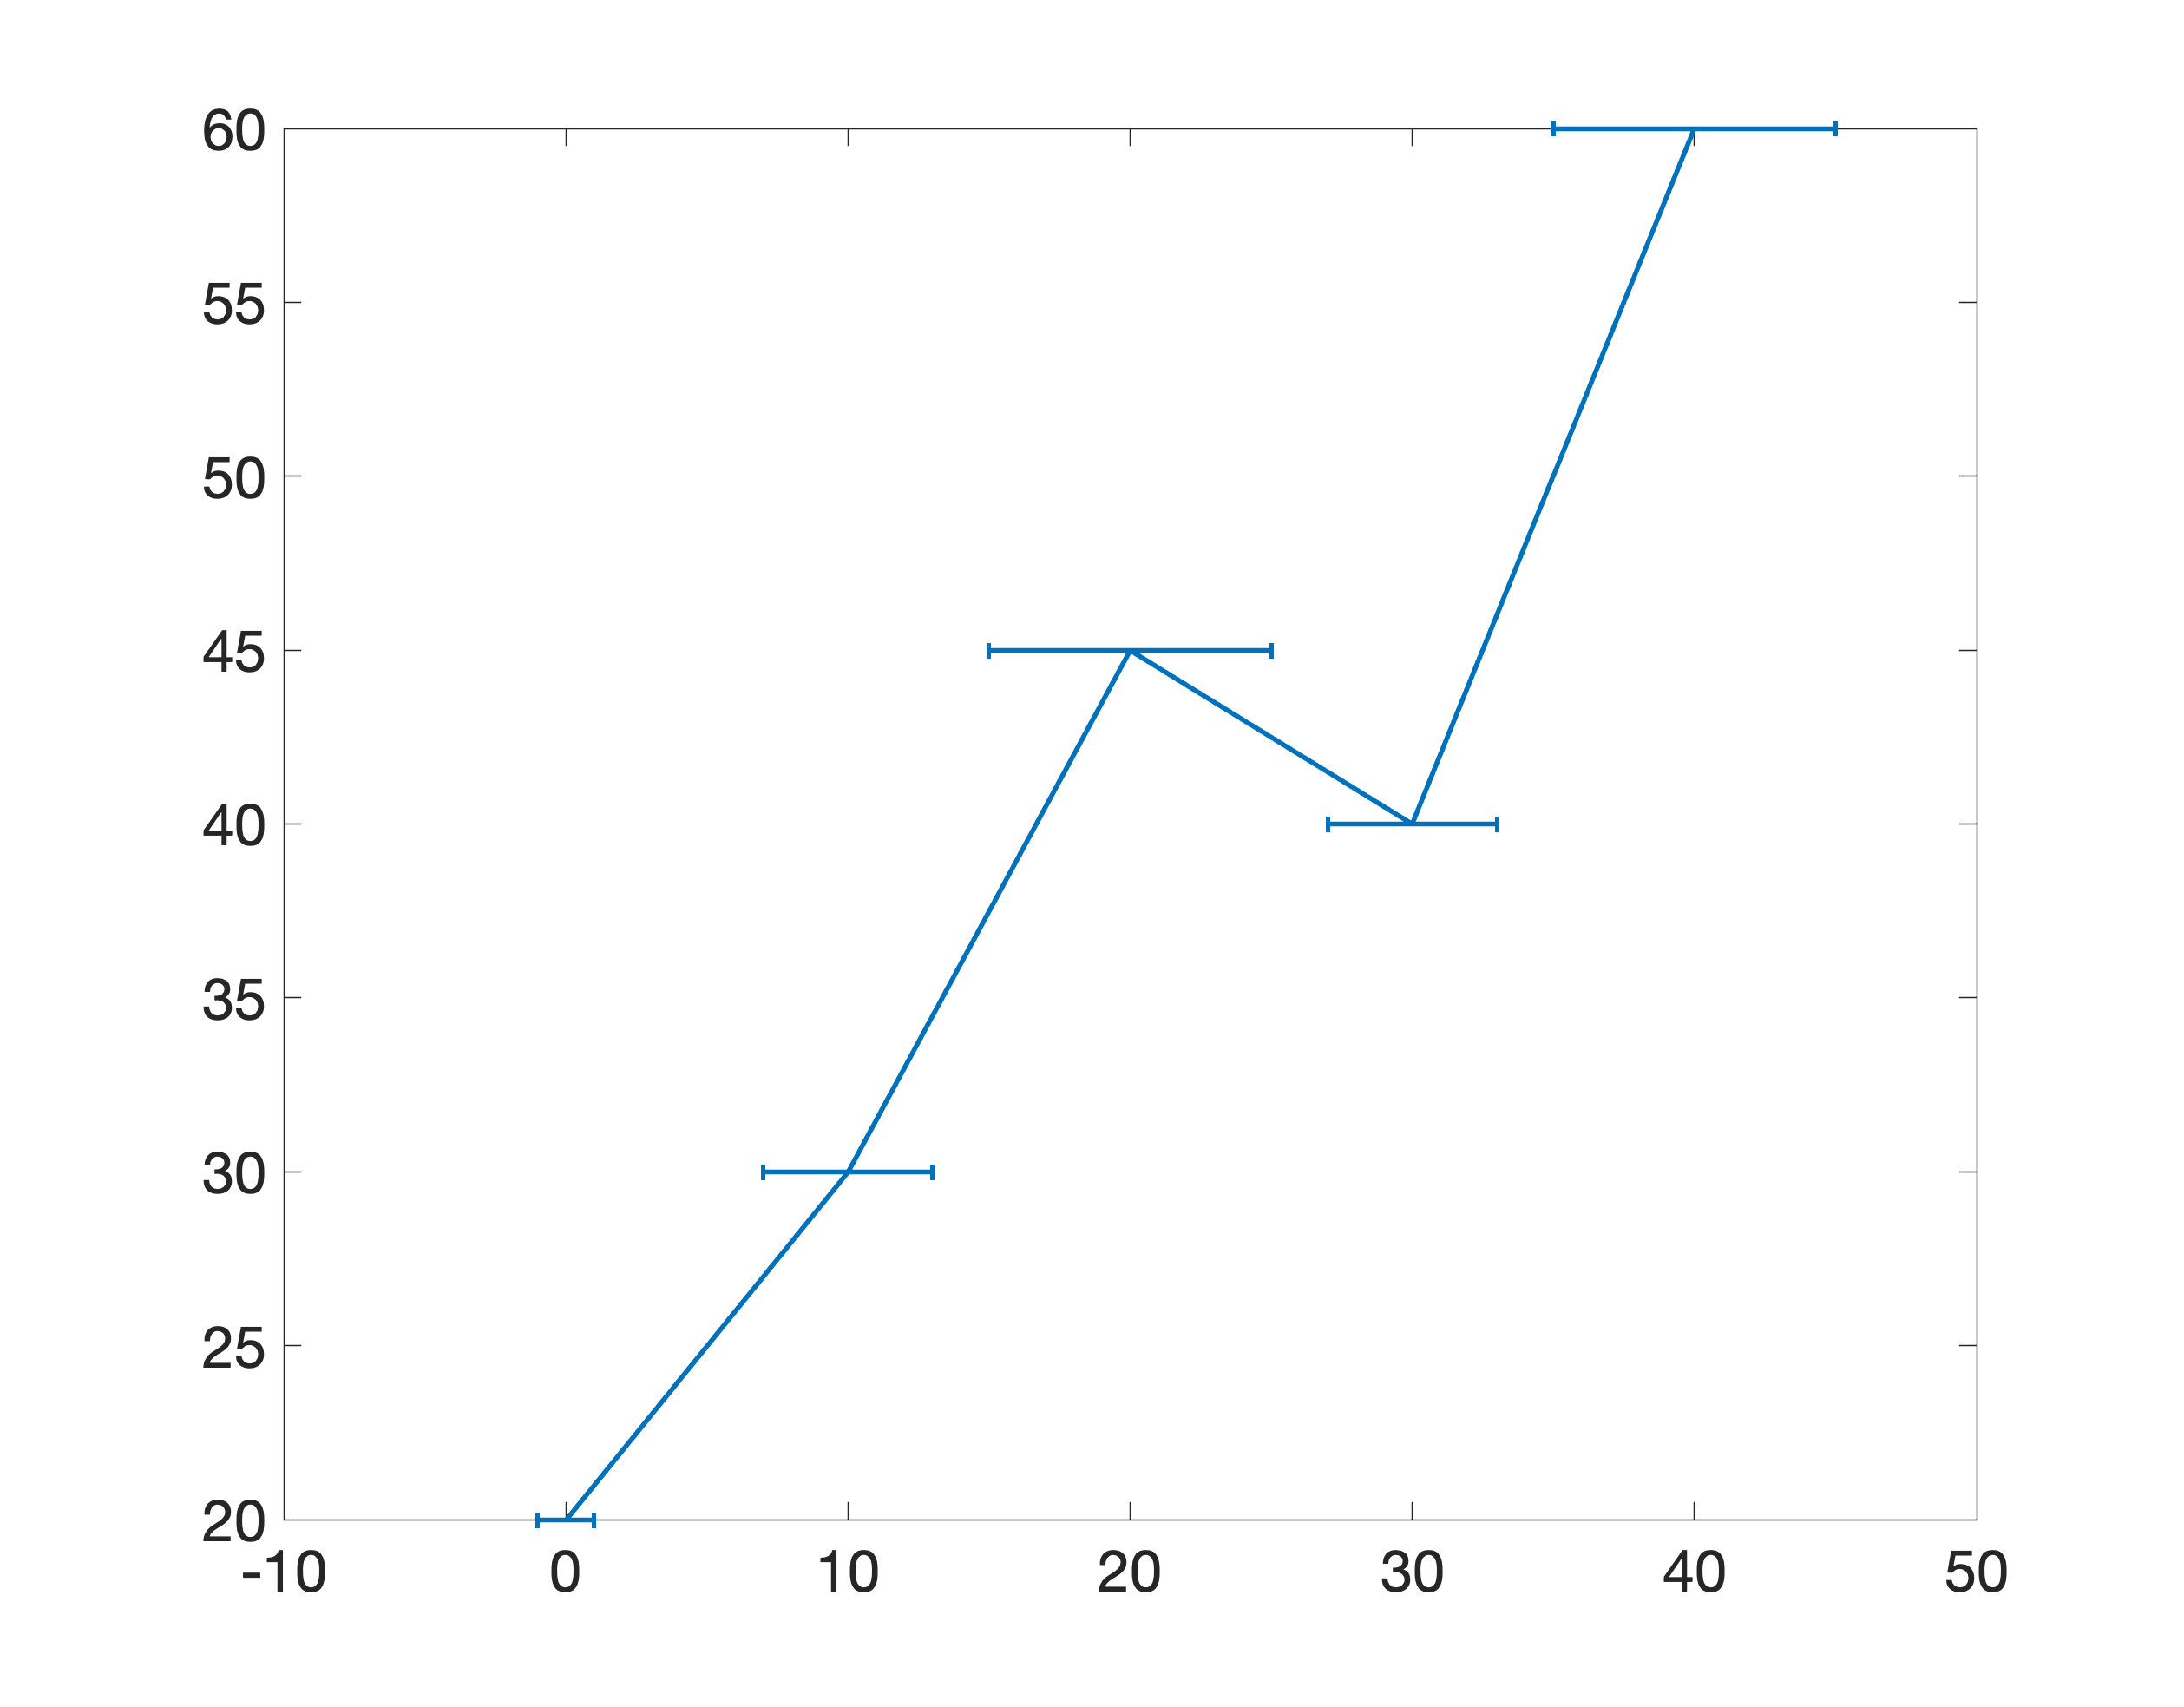
\includegraphics[width=1\linewidth]{./error2.png}
\end{columns}    
\end{frame}

\begin{frame}[c,fragile]
\frametitle{График с оценкой погрешности}
\begin{columns}
\column{.5\textwidth}
\begin{lstlisting}
x = 1:10:100;
y = [20 30 45 40 60 65...
     80 75 95 90];
yneg = [1 3 5 3 5 3 6 4 3 3];
ypos = [2 5 3 5 2 5 2 2 5 5];
xneg = [1 3 5 3 5 3 6 4 3 3];
xpos = [2 5 3 5 2 5 2 2 5 5];
errorbar(x,y,yneg,ypos,...
         xneg,xpos,'o:');
\end{lstlisting}
\column{.5\textwidth}
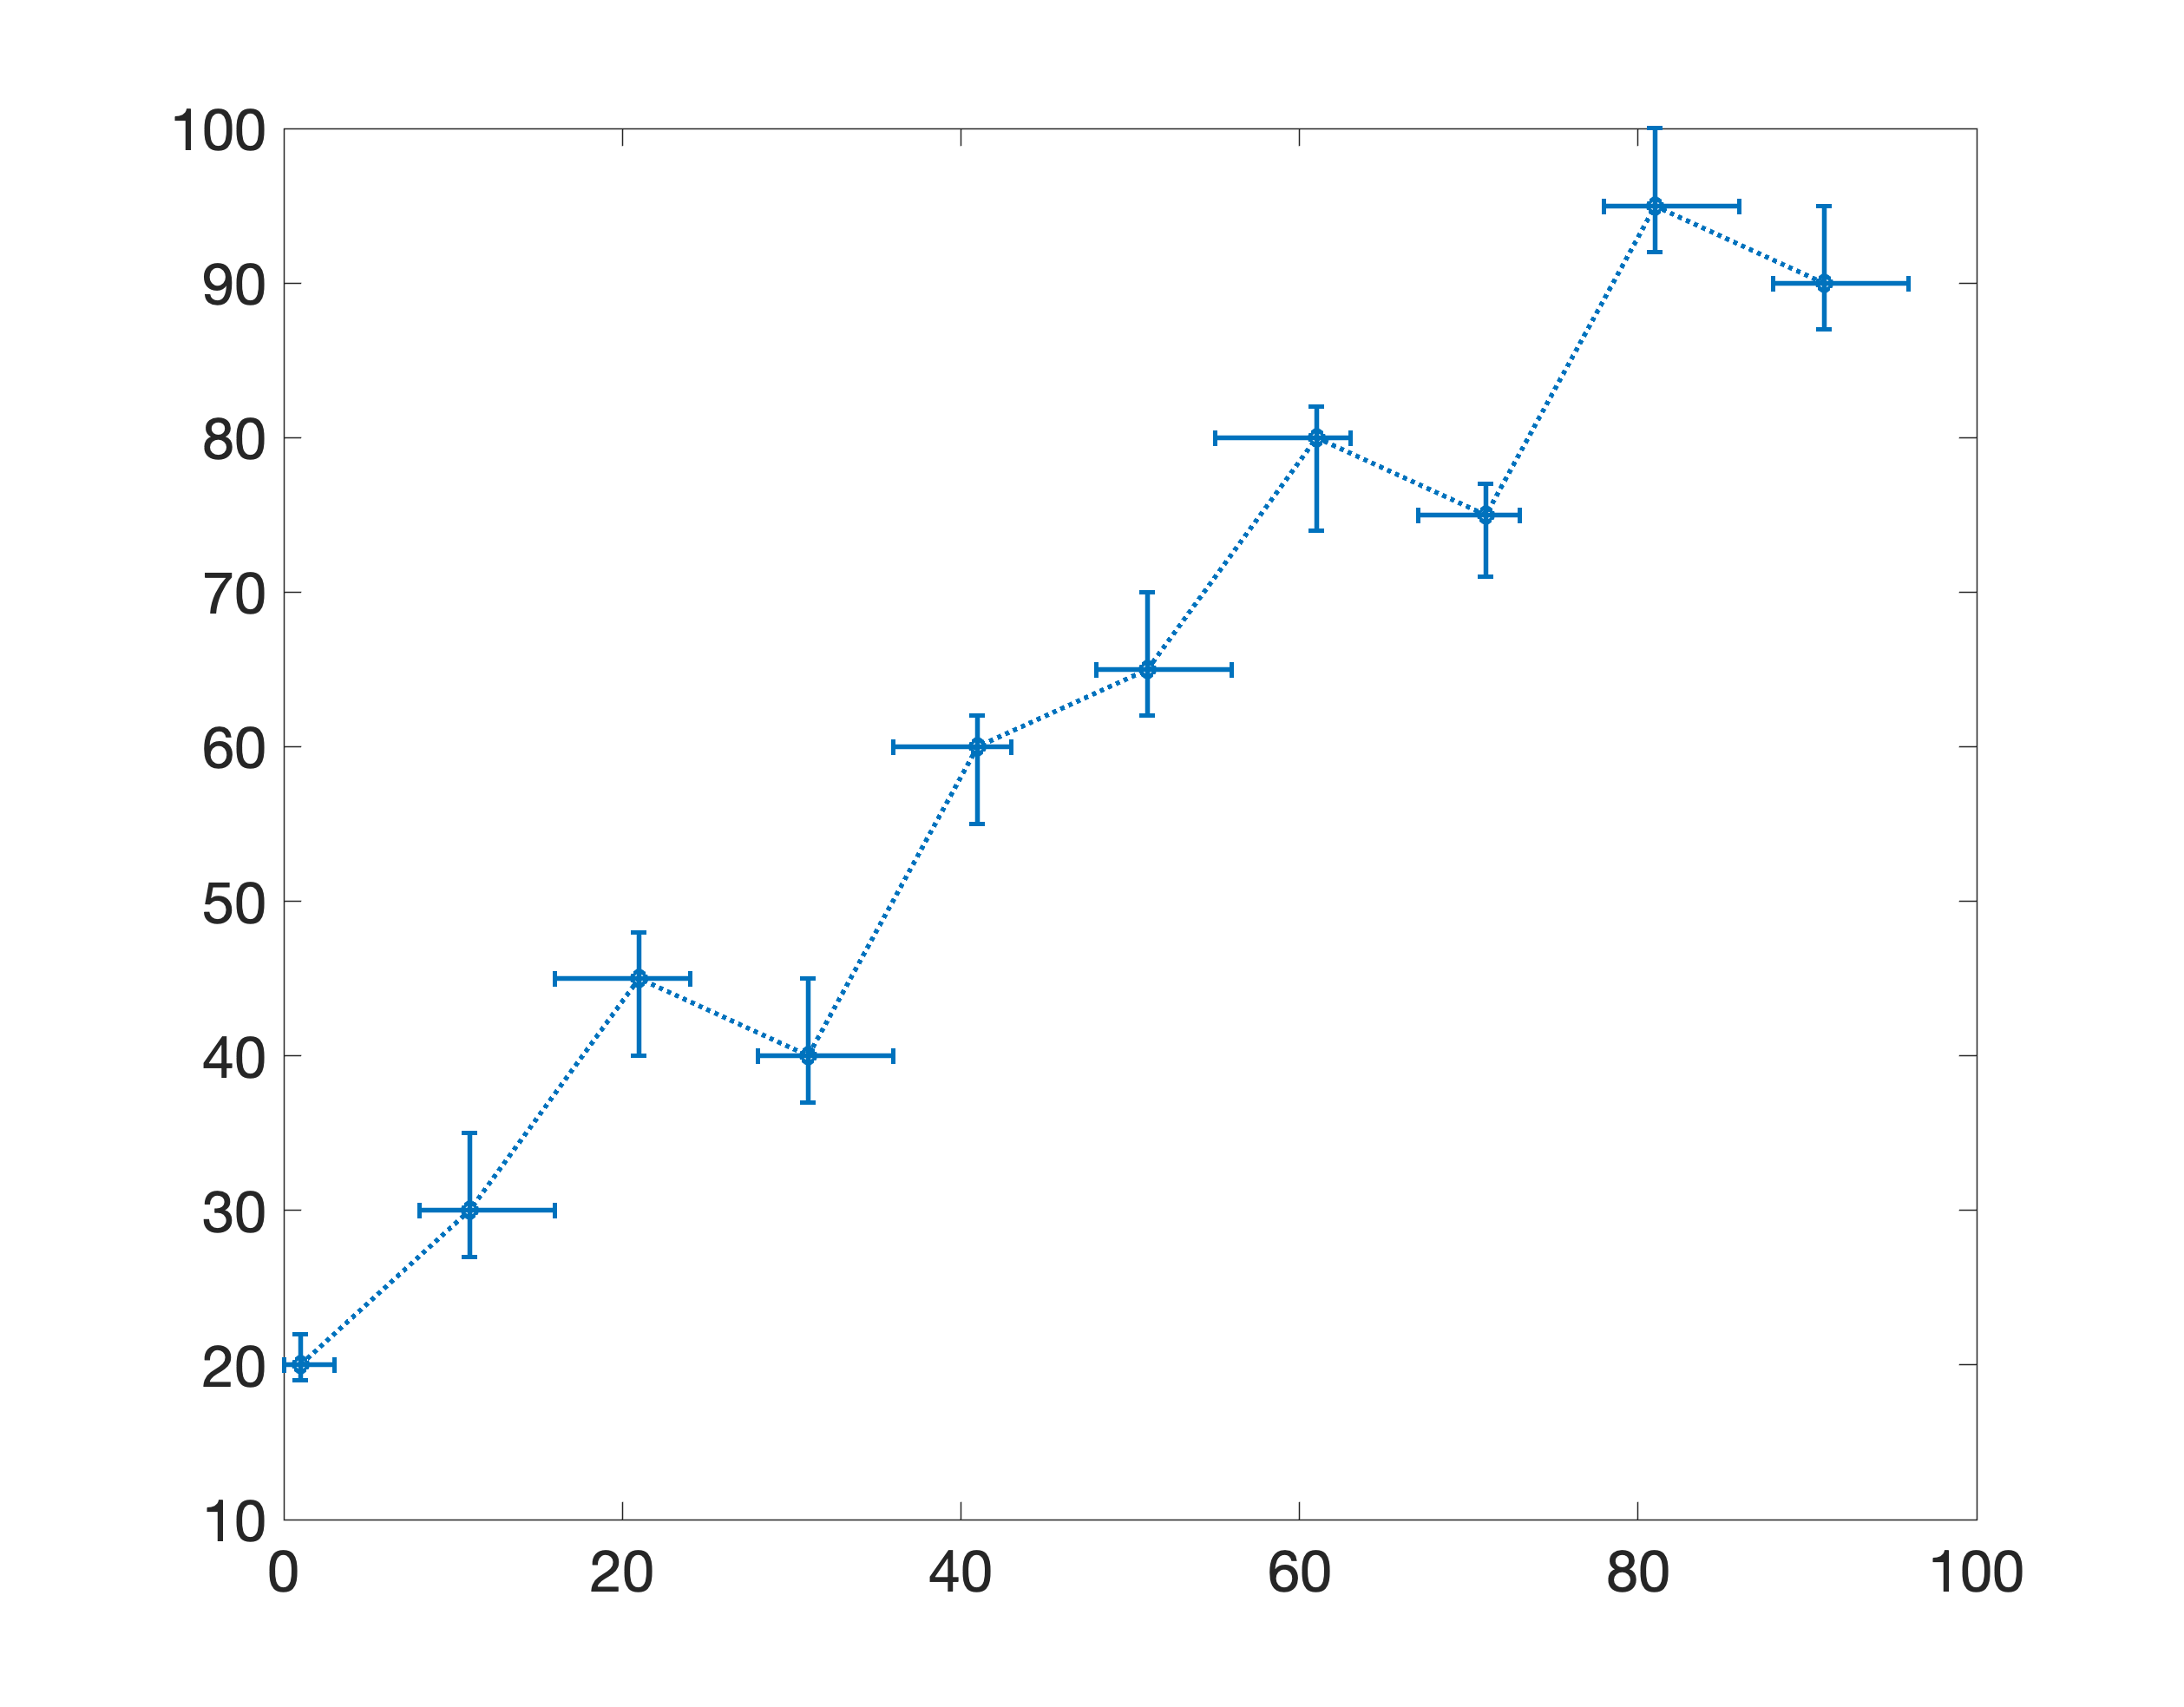
\includegraphics[width=1\linewidth]{./error3.png}
\end{columns}    
\end{frame}

% \section{Функции двух переменных}

\frame[containsverbatim]
{
\frametitle{Сетки и поверхности}
\begin{columns}
\column{.5\textwidth}
\begin{lstlisting}
pp=-1:0.1:1;
[X,Y]=meshgrid(pp,pp);
Z=X.^2+Y.^2;
mesh(X,Y,Z);
colorbar;
\end{lstlisting}
или (раскрашенная сеточная поверхность)
\begin{lstlisting}
surf(X,Y,Z);
\end{lstlisting}
\column{.5\textwidth}
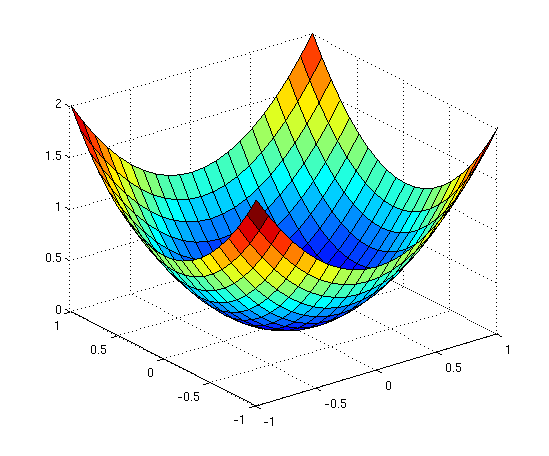
\includegraphics[width=1\linewidth]{./surf.png}
\end{columns}
}

\frame[containsverbatim]
{
\frametitle{Функция meshgrid}
\begin{lstlisting}
[x, y] = meshgrid(0:0.1:0.4,  0:0.2:0.4);

x =

         0    0.1000    0.2000    0.3000    0.4000
         0    0.1000    0.2000    0.3000    0.4000
         0    0.1000    0.2000    0.3000    0.4000


y =

         0         0         0         0         0
    0.2000    0.2000    0.2000    0.2000    0.2000
    0.4000    0.4000    0.4000    0.4000    0.4000
\end{lstlisting}
}


\frame[containsverbatim]
{
\frametitle{Контурные графики}
\begin{lstlisting}
[X,Y]=meshgrid(-1:0.1:1,-1:0.1:1);
Z=X.^2+Y.^2;
contour(X,Y,Z);
[c,h]=contour(X,Y,Z));
clabel(c,h); grid on;
\end{lstlisting}
\begin{center}
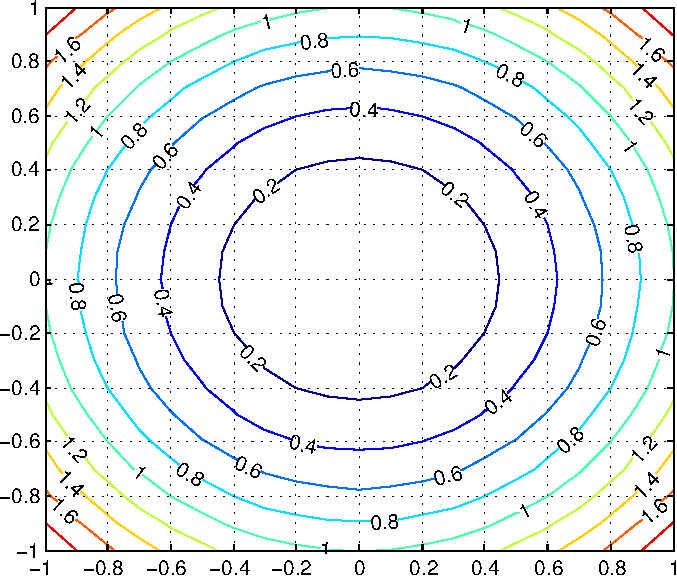
\includegraphics[width=0.5\linewidth]{./contourplot.pdf}
\end{center}
}

\frame[containsverbatim]
{
\frametitle{Контурный график с заливкой}
\begin{columns}
\column{.5\textwidth}
\begin{lstlisting}
contourf(X,Y,Z,10); 
colorbar;
\end{lstlisting} 
\column{.5\textwidth}
\begin{figure}[t]
 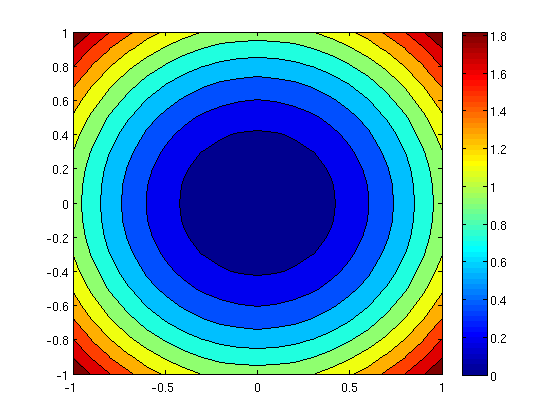
\includegraphics[width=1\linewidth]{./contourf.png}
\end{figure}
\end{columns}
}

\frame[containsverbatim]
{
\frametitle{Палитра}
\begin{columns}
\column{.6\textwidth}
\begin{lstlisting}
contourf(X,Y,Z,10);
colorbar;
\end{lstlisting} 
\column{.4\textwidth}
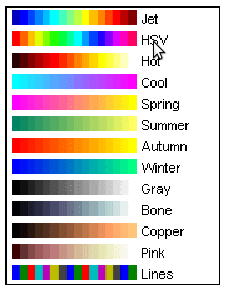
\includegraphics[width=1\linewidth]{./colormap.png}
\end{columns}
}

\frame[containsverbatim]
{
\frametitle{Палитра}
\begin{columns}
\column{.5\textwidth}
\begin{lstlisting}
pp=-1:0.1:1;
[X,Y]=meshgrid(pp,pp);
Z=-X.^2-Y;
contourf(X,Y,Z,12);
colorbar;
colormap(gray);  
title('z=x^2+y^2');   
\end{lstlisting}
\column{.5\textwidth}
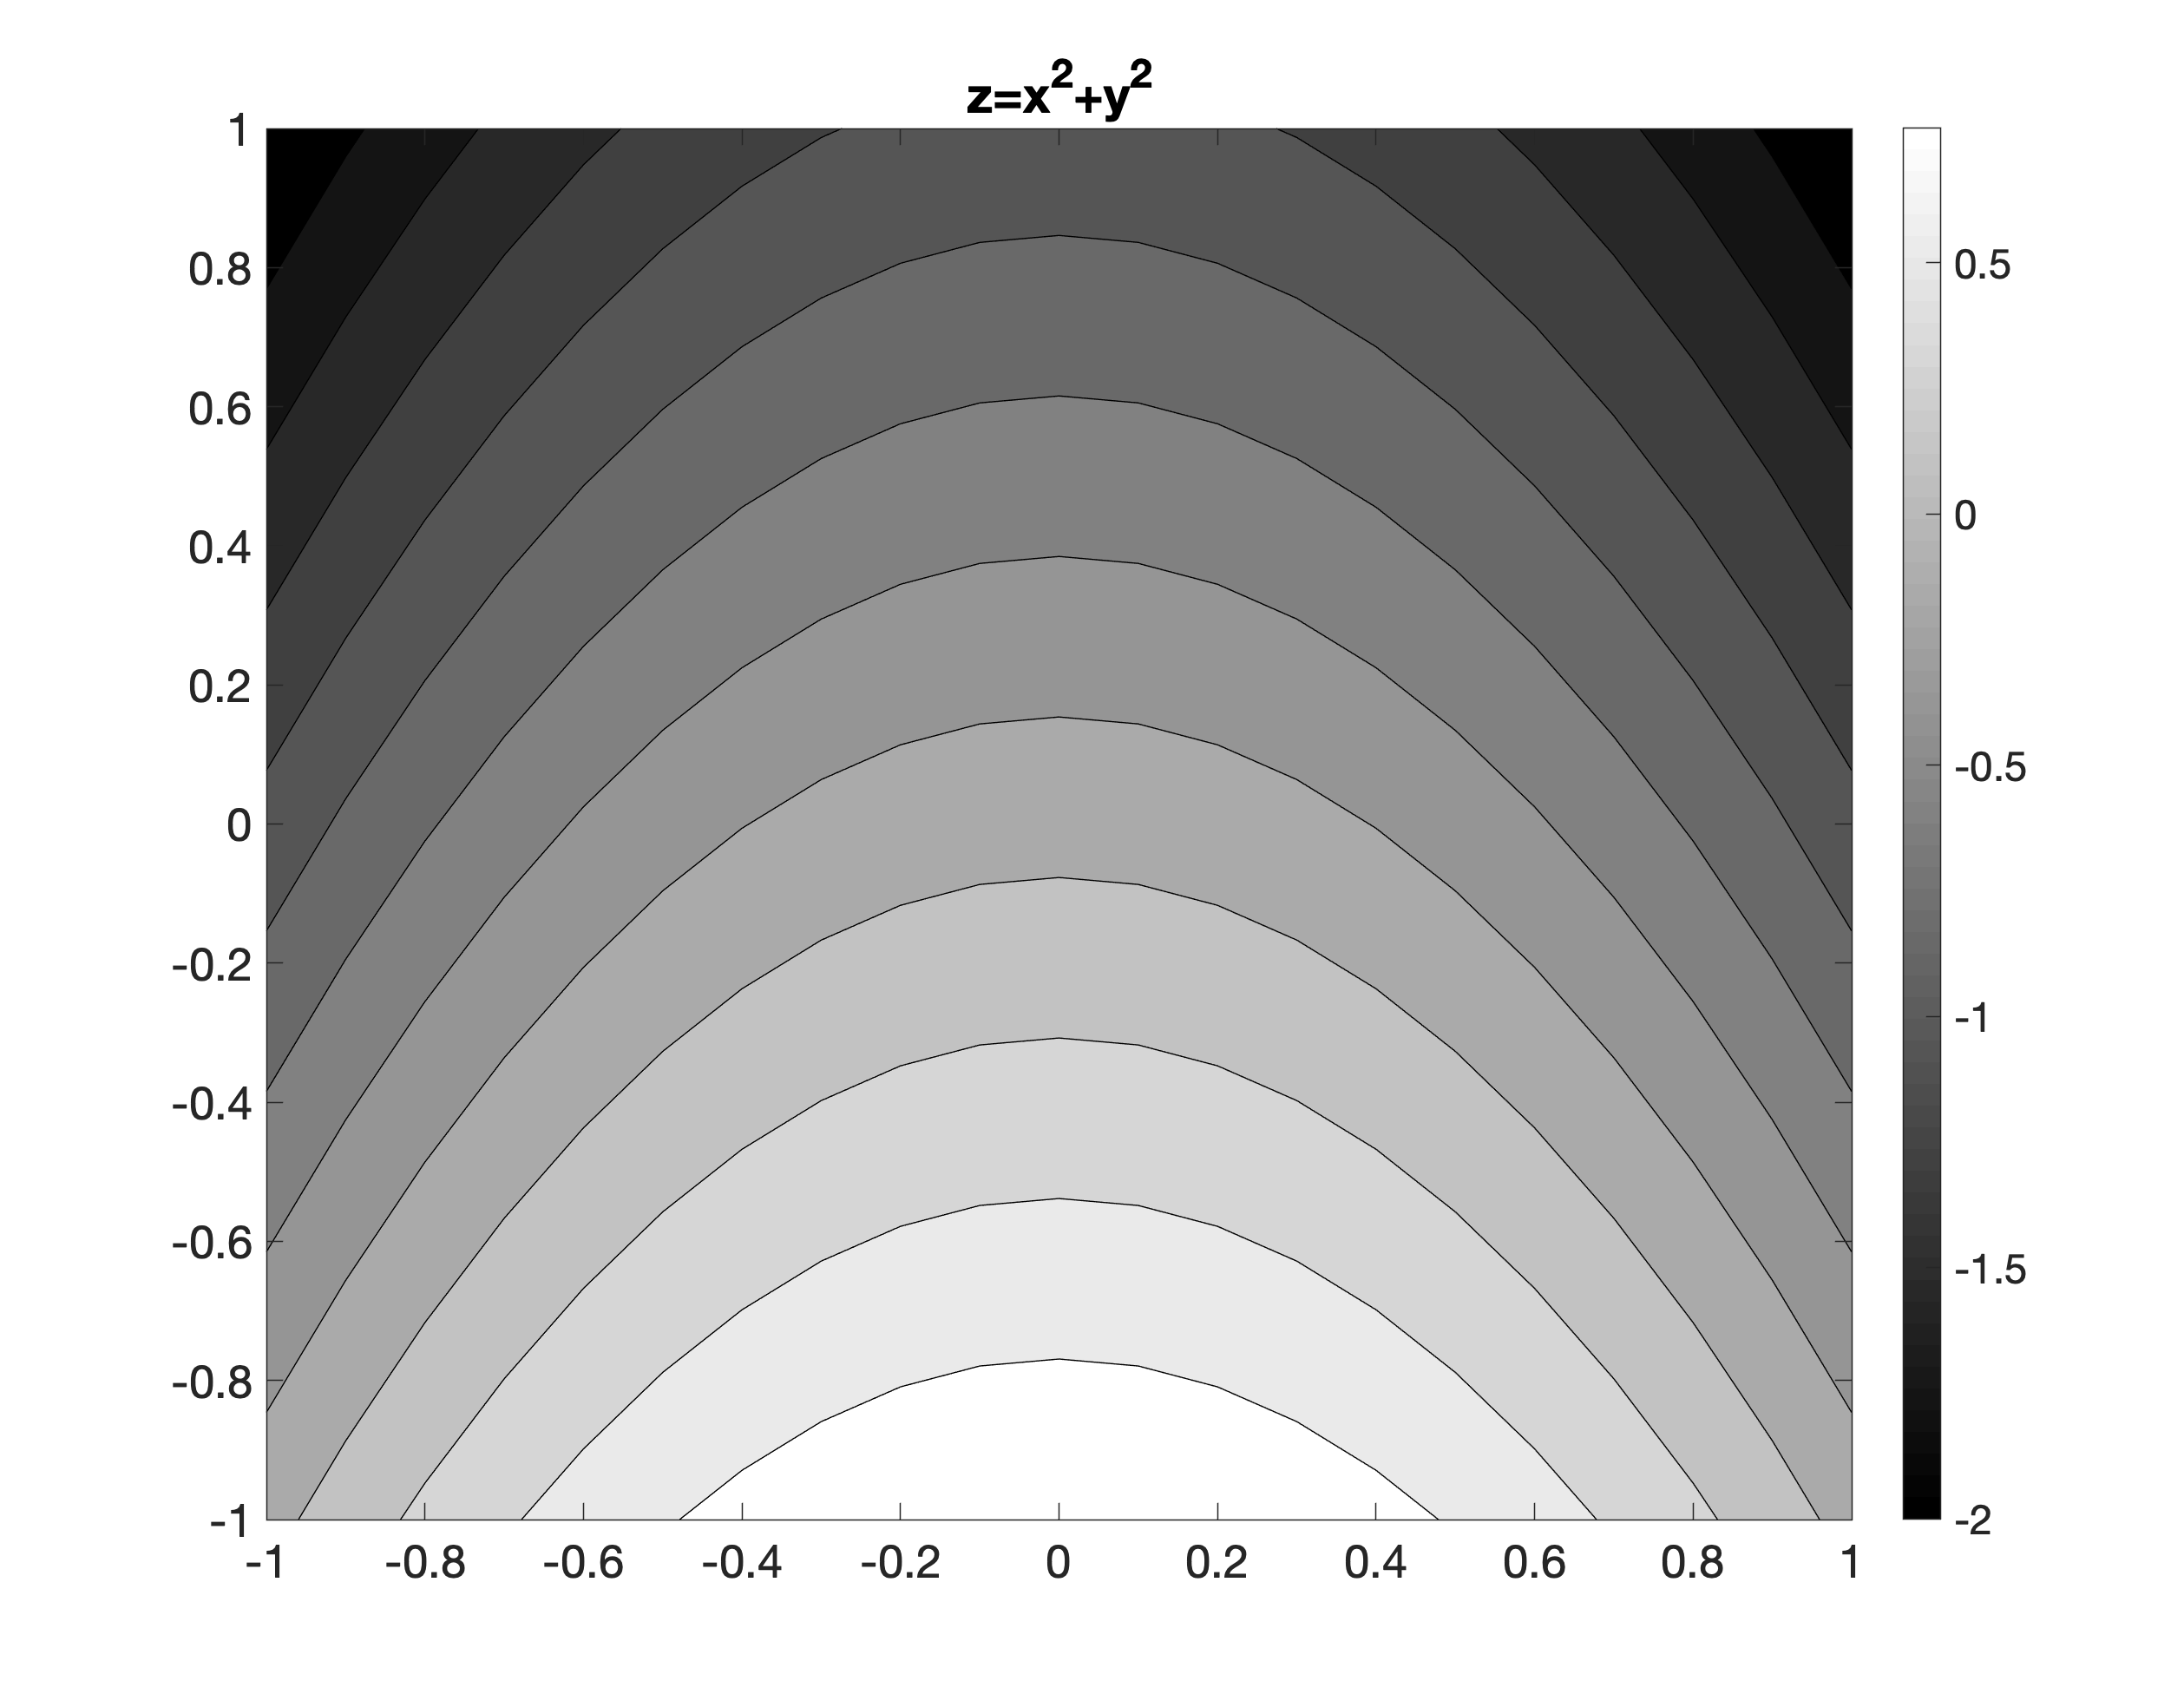
\includegraphics[width=1\linewidth]{./contourf_gray.png}
\end{columns}
}


\frame[containsverbatim]
{
\frametitle{Параметрические кривые в пространстве}
\begin{columns}
\column{.5\textwidth}
\begin{lstlisting}
t=0:0.1:20;
x=cos(t);
y=sin(t);
z=t;
plot3d(x,y,z);
\end{lstlisting} 
\column{.5\textwidth}
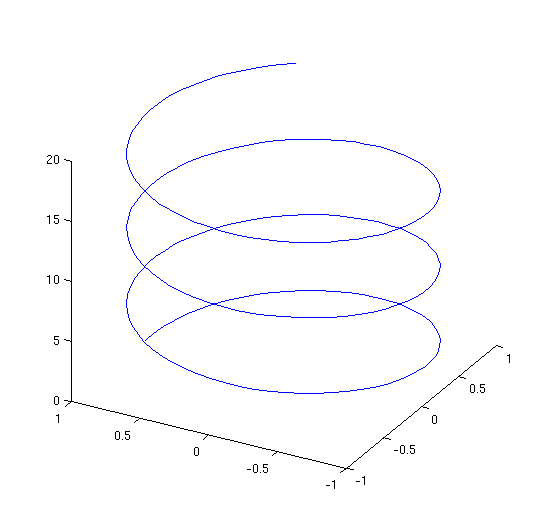
\includegraphics[width=1\linewidth]{./plot3d.png}
\end{columns}
}

\frame[containsverbatim]
{
\frametitle{Поворот пространственного графика}
\begin{columns}
\column{.5\textwidth}
Задать новое положение наблюдателя:
\begin{lstlisting}
view(az,el);
\end{lstlisting}
Определить положение наблюдателя
\begin{lstlisting}
[Az,El]=view;
\end{lstlisting}
Взгляд направлен вдоль оси y
\begin{lstlisting}
view(0,0);
\end{lstlisting}
\column{.5\textwidth}
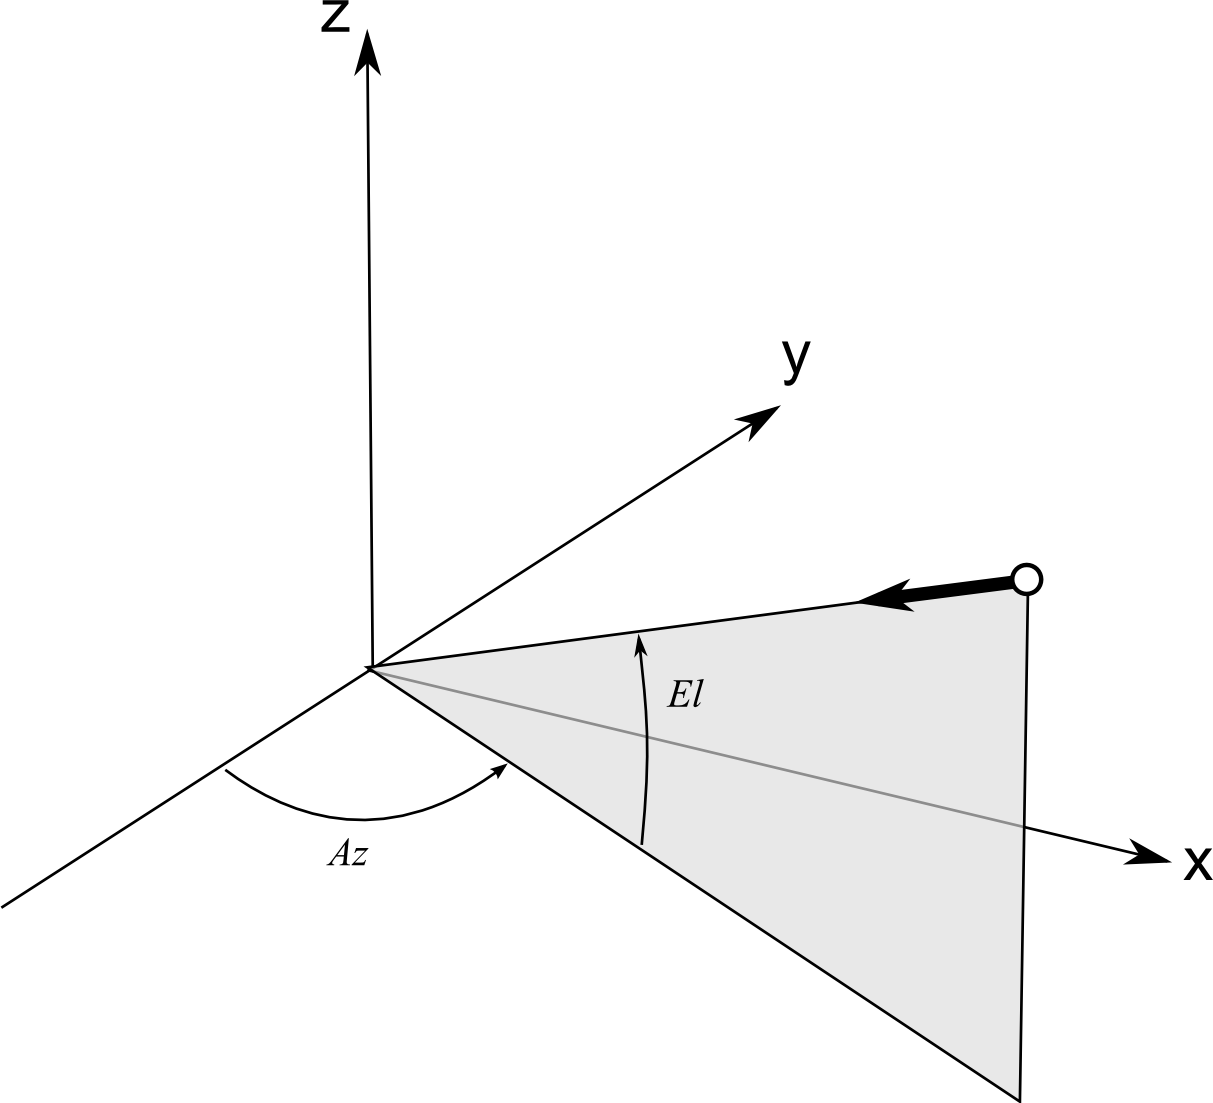
\includegraphics[width=1\linewidth]{./AzEl.png}
\end{columns}
}

\frame[containsverbatim]
{
\frametitle{Освещенная поверхность}
\begin{columns}
\column{.5\textwidth}
Отобразить поверхность с заданным азимутом и возвышением источника света:
\begin{lstlisting}
surfl(X,Y,Z,[Az,El]);
\end{lstlisting}
Палитра copper:
\begin{lstlisting}
colormap('copper');
\end{lstlisting}
Сглаживать цвета:
\begin{lstlisting}
shading interp;
\end{lstlisting}
\column{.5\textwidth}
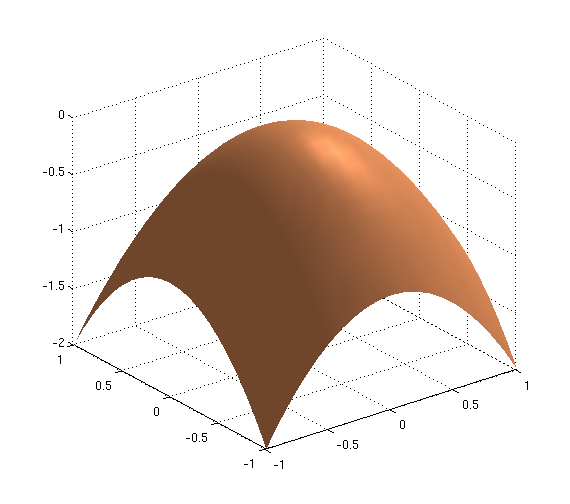
\includegraphics[width=1\linewidth]{./surfl.png}
\end{columns}
}


\frame[containsverbatim]
{
\frametitle{Анимированные графики. Функция comet}
На плоскости:
\begin{lstlisting}
t=0:0.01:10;
x=t-sin(t);
y=1-cos(t);
comet(x,y);
\end{lstlisting}
В пространстве:
\begin{lstlisting}
t=0:0.01:10;
x=cos(t);
y=sin(t);
z=t;
comet3(x,y,z);
\end{lstlisting}  
}

\begin{frame}[c,fragile]
\frametitle{Экспорт в файл}
Экпорт в растровый формат (png)
\begin{lstlisting}
t=0:0.01:10;
x=cos(t);
y=sin(t);
plot(x,y);

print('filename','-dpng','-r300');      
\end{lstlisting}

Экпорт в векторный формат (pdf)
\begin{lstlisting}
figure('PaperUnits','Centimeters','PaperSize',[16,10]);
t=0:0.01:10;
x=cos(t);
y=sin(t);
plot(x,y);

print('plot_figure','-dpdf','-fillpage');
\end{lstlisting}
\end{frame}




\end{document}
